%%%%%%%%%%%%%%%%%%%%%%%%%%%%%%%%%%%%%%%%%%%%%%%%%%%%%%%%%%%%%%%%%%%%%%
%%%%%%%%%%%%%%%%%%%%%%%%%%%%%%%%%%%%%%%%%%%%%%%%%%%%%%%%%%%%%%%%%%%%%%
%%%%%%%%%%%%%%%%%%%%%%%%%%%%              SOFTWARE           %%%%%%%%%%%%%%%%%%%%%%%%%%%%
%%%%%%%%%%%%%%%%%%%%%%%%%%%%%%%%%%%%%%%%%%%%%%%%%%%%%%%%%%%%%%%%%%%%%%
%%%%%%%%%%%%%%%%%%%%%%%%%%%%%%%%%%%%%%%%%%%%%%%%%%%%%%%%%%%%%%%%%%%%%%
\section{Software}

The main analysis tasks (\texttt{C++} classes) used in the analysis are in the \texttt{PWGJE} library of the \texttt{AliPhysics} software package:
\begin{itemize}
\item \texttt{AliAnalysisTaskSEDmesonsFilterCJ} (filters D mesons and create a set of particles with the D meson instead of the daughters);
\item \texttt{AliAnalysisTaskFlavourJetCorrelations} (correlates each found D meson with a jet);
\item \texttt{AliEmcalJetTask};
\item \texttt{AliAnalysisTaskRhoSparse}.
\end{itemize}
The \texttt{AliPhysics} version used for this analysis is the analysis tag: \texttt{vAN-20170826} (with \texttt{AliRoot v5-09-14-1}).

The task used for this analysis generates a multiple axis histogram (\texttt{THnSparse}) that keep informations about: \zpar, jet \pt, D-meson \pt\ and D-meson invariant mass.

The post-processing includes: projection of the \texttt{THnSparse} into lower-dimensional histograms, raw signal extraction, response matrix generation, unfolding, B feed-down correction and the final plotting.
The post-processing is relatively light-weight and is performed directly in a personal computer. This code is written using the \texttt{C++} with \texttt{ROOT}.

%The code is fully available in a \texttt{GIT} repository hosted on the CERN \texttt{Gitlab} service: 
%\url{https://gitlab.cern.ch/saiola/alice-yale-hfjet}. In particular the code is organized as follows:
%\begin{itemize}
%\item \texttt{DMesonJetAnalysis}: main post-processing software (tree projection, raw signal extraction, unfolding);
%\item \texttt{fastSimulation}: scripts to run fast simulations locally or on the grid (used for the estimation of the B feed-down correction);
%\item \texttt{merging}: scripts to merge and download results from the grid;
%\item \texttt{anaDev}: scripts to test the analysis tasks.
%\end{itemize}
%

%%%%%%%%%%%%%%%%%%%%%%%%%%%%%%%%%%%%%%%%%%%%%%%%%%%%%%%%%%%%%%%%%%%%%%
%%%%%%%%%%%%%%%%%%%%%%%%%%%%%%%%%%%%%%%%%%%%%%%%%%%%%%%%%%%%%%%%%%%%%%
%%%%%%%%%%%%%%%%%%%%%%%%%%%%              DATASETS            %%%%%%%%%%%%%%%%%%%%%%%%%%%%
%%%%%%%%%%%%%%%%%%%%%%%%%%%%%%%%%%%%%%%%%%%%%%%%%%%%%%%%%%%%%%%%%%%%%%
%%%%%%%%%%%%%%%%%%%%%%%%%%%%%%%%%%%%%%%%%%%%%%%%%%%%%%%%%%%%%%%%%%%%%%

\section{Dataset and Event Selection}

For this analysis we use the data collected by ALICE in 2016 during the Minimum Bias period of the \pPb\ collisions at $\snn=5.02$~TeV. These data corresponds to the following data taking periods:
LHC16q and LHC16t pass1, FAST and CENT\_woSDD productions were merged, the total number of events is 603.1 M (after all the selections outlined below) out of 834.5 M analysed.
The complete list of runs used in this analysis is:

LHC16q: 265525, 265521, 265501, 265500, 265499, 265435, 265427, 265426, 265425, 265424, 265422, 265421, 265420, 265419, 265388, 265387, 265385, 265384, 265383, 265381, 265378, 265377, 265344, 265343, 265342, 265339, 265338, 265336, 265335, 265334, 265332, 265309  \\
LHC16t: 267166, 267165, 267164, 267163 

Events were selected using the event selection \texttt{kINT7}. Note that the analysis is performed in \texttt{AOD}, where the beam-gas and gas-gas events have been filtered out.
Events were further filtered using the Physics Selection, and selection provided by:
\begin{itemize}
\item \texttt{AliAnalysisTaskEmcal::IsEventSelected()}, which rejects events based on event vertex quality, in particular requiring a reconstructed vertex position not farther than 10 cm from the center of the detector along the beam axis; and a distance between the SPD vertex and the V0 vertex not larger than 0.5 cm %($2.75+8.66+34.41+29.74$~M~$=75.56$~M events rejected);
\item \texttt{AliRDHFCutsDStartoKpipi::IsEventSelected(AliVEvent*)}, which rejects events based on event vertex quality 
%($0.68+1.90+3.71+3.03$~M~$= 9.32$~M events rejected) 
and pileup 
%($0.09+1.07+1.65+1.18$~M~$ =  3.99$~M events rejected).
\end{itemize}

Results shown below come from the LEGO trains HFCJ\_pPb: \\343 (LHC16q\_pass1\_FAST), 344 (LHC16q\_pass1\_CENT\_woSDD), 345 ( LHC16t\_pass1\_FAST) and 346 (LHC16t\_pass1\_CENT\_woSDD).

\subsubsection{Monte Carlo productions}

For this analysis the Monte Carlo production LHC17d2a\_fast\_new has been used, anchored to the 2016 \pPb\ data taking periods LHC16q and LHC16t and the FAST production. The FAST production simulation is used to corrected the datasample, which is merged FAST+CENT\_woSDD, assuming that efficiencies are detector response are the same for both.
The simulations uses PYTHIA6 with the Perugia2011 tune as particle generator at $\s=5.02$~TeV. If $N_{coll} > $ 1, the even generated by Hijing is also embedded.
The charm content has been enhanced by requesting a \ccbar\ in 50\% of the events and a \bbbar\ in the remaining half.
Furthermore, all D mesons are forced to decay hadronically.
This MC production is used to compute the D-meson efficiency with jets, acceptance corrections and a response matrix of D-tagged jets with prompt and non-prompt \Dstar: c,~b~$\rightarrow$~\Dstar.

Results shown below come from the LEGO trains HFCJ\_pPb\_MC: 77 (full simulation), and 76 (only Pythia part of the simulation).


%%%%%%%%%%%%%%%%%%%%%%%%%%%%%%%%%%%%%%%%%%%%%%%%%%%%%%%%%%%%%%%%%%%%%%
%%%%%%%%%%%%%%%%%%%%%%%%%%%%%%%%%%%%%%%%%%%%%%%%%%%%%%%%%%%%%%%%%%%%%%
%%%%%%%%%%%%%%%%%%%%%%%%%%%%    D-MESON SELECTION   %%%%%%%%%%%%%%%%%%%%%%%%%%%%
%%%%%%%%%%%%%%%%%%%%%%%%%%%%%%%%%%%%%%%%%%%%%%%%%%%%%%%%%%%%%%%%%%%%%%
%%%%%%%%%%%%%%%%%%%%%%%%%%%%%%%%%%%%%%%%%%%%%%%%%%%%%%%%%%%%%%%%%%%%%%

\section{D-Meson Selection}
\label{sec:DmesonSel}
The \Dstar mesons were reconstructed through their hadronic decay channels~\cite{PDG:2016}:

\begin{center}
$\Dstar \to \Dzero + \pi^{\pm} \to {\rm K}^{\pm} + \pi^{\mp}  + \pi^{\pm}$ , BR = 67.7$\pm$0.5\%, 3.93$\pm$0.04\%
\end{center}

The selection strategy is based on the topological displacement of the secondary vertex from the primary vertex due to their relatively large lifetime.

The candidate vertices are read from the \texttt{AOD} friend chain \texttt{AliAOD.VertexingHF.root}. A list of topological and kinematic cuts applied for \Dstar\ in \pPb\ collisions at $\snn=5.02$~TeV can be found in Table~\ref{DStarCutspPb}.
The same quality track selection on the decay products used for the D-meson spectra analysis of the same datasets has been used in this analysis.
For the final jet spectrum we will apply $\ptd> 3$~\GeVc\ on the D mesons. The accepted $|y_{\rm D}|$ range is \pt-dependent, with the upper limit growing from $0.5$ to $0.8$ at $\pt=5$~\GeVc.

    
    \begin{table}[bth]
\caption{\Dstar\ cuts for \pPb\ collisions at $\snn=5.02$~TeV.}
     \label{DStarCutspPb}
\begin{center}
\begin{scriptsize}
    \begin{tabular}{lrrrrrrrrrrrrr}
    \hline
    $p_{\mathrm T,\Dzero}$ (\GeVc) & $0.5-1$ & $1-2$ & $2-3$ & $3-4$ & $4-5$ & $5-6$ & $6-7$ & $7-8$ & $8-10$ & $10-12$ & $12-16$ & $16-24$ & $24-36$ \\ \hline
    $\Delta M_{\Dzero} (\GeVcsq)$ & 0.03 & 0.032 & 0.032 & 0.032 & 0.032 & 0.036 & 0.036 & 0.036 & 0.05 & 0.05 & 0.094 & 0.094 & 0.7 \\ \hline
    DCA (cm) & 0.0315 & 0.025 & 0.03 & 0.03 & 0.035 & 0.04 & 0.08 & 0.12 & 0.12 & 0.12 & 0.2 & 0.2 & 0.5 \\ \hline
    $\cos(\theta^{*})$ & 0.9 & 0.8 & 0.8 & 0.8 & 0.9 & 1 & 1 & 1 & 1 & 1 & 1 & 1 & 1\\ \hline
    $p_{\mathrm T,K}$ (\GeVc) & 0.5 & 1 & 1 & 1 & 1 & 1 & 1 & 1 & 1 & 1 & 0.3 & 0.3 & 0 \\ \hline
    $p_{\mathrm T,\pi}$ (\GeVc) & 05 & 1 & 1 & 1 & 1 & 1 & 1 & 1 & 1 & 1 & 0.3 & 0.3 & 0 \\ \hline
    $d_{0}^{K}$  (cm) & 0.1 & 0.1 & 0.1 & 0.1 & 0.1 & 0.1 & 0.1 & 0.1 & 0.1 & 0.1 & 0.2 & 0.2 & 999 \\ \hline
    $d_{0}^{\pi}$  (cm) & 0.1 & 0.1 & 0.1 & 0.1 & 0.1 & 0.1 & 0.1 & 0.1 & 0.1 & 0.1 & 0.2 & 0.2 & 999 \\ \hline
    $d_{0}^{K}\cdot d_{0}^{\pi}$ $(10^{-4}{\rm cm}^2)$ & -3 & -2 & -2.5 & -1.3 & -0.38 & 0.44 & 5 & 5 & 100 & 100 & 500 & 1000 & 1000 \\ \hline
    $\cos(\theta_{\rm point})$ & 0.8 & 0.9 & 0.9 & 0.87 & 0.86 & 0.83 & 0.76 & 0.76 & 0.68 & 0.68 & 0.60 & -1 & -1 \\ \hline
    $\cos(\theta_{{\rm point},xy})$ & - & 0.97 & - & - & - & - & - & - & - & - & - & - & - \\ \hline
    $L_{xy ({\rm cm})}$ & 4 & 3.5 & 4 & 3.5 & 3 & 2.5 & 1.5 & 1 & 0 & 0 & 0 & 0 & 0 \\ \hline
    \end{tabular}
    \end{scriptsize}
    \end{center}
    \end{table}

\subsection{Particle Identification}

The Particle Identification (PID) of pions and kaons was performed using the information of the specific energy loss 
in the TPC and the time of flight provided by the TOF detector. 
In order to identify a track as a pion or a kaon its TPC \dedx\ and/or time-of-flight were required to be within 3$\sigma$ of the expected values. 
Tracks with no TOF information were identified using only the TPC.
Tracks compatible with both the kaon and the pion hypotheses were retained for analysis and both mass hypotheses were considered.

%%%%%%%%%%%%%%%%%%%%%%%%%%%%%%%%%%%%%%%%%%%%%%%%%%%%%%%%%%%%%%%%%%%%%%
%%%%%%%%%%%%%%%%%%%%%%%%%%%%%%%%%%%%%%%%%%%%%%%%%%%%%%%%%%%%%%%%%%%%%%
%%%%%%%%%%%%%%%%%%%%%%%%%%%%  JET RECONSTRUCTION  %%%%%%%%%%%%%%%%%%%%%%%%%%%%
%%%%%%%%%%%%%%%%%%%%%%%%%%%%%%%%%%%%%%%%%%%%%%%%%%%%%%%%%%%%%%%%%%%%%%
%%%%%%%%%%%%%%%%%%%%%%%%%%%%%%%%%%%%%%%%%%%%%%%%%%%%%%%%%%%%%%%%%%%%%%

\section{Jet Reconstruction}

The \texttt{FASTJET}\cite{Cacciari:2012} package was used to reconstruct the jets. 
In particular, the \antikt\ algorithm~\cite{Cacciari:2008c} was employed to reconstruct signal jets. 
This algorithm is infrared-safe (not sensitive to low energy radiations) and collinear-safe (not sensitive to collinear particle splitting).
A resolution parameter of $R=0.4$ was used for both the \pPb\ analyses.
In the \pPb\ analysis, the \kt\ algorithm~\cite{Cacciari:2006} was employed to estimate the background. 
For this analysis, only charged tracks are used to reconstructed the jets (\emph{charged jets}).

The set of tracks given as input to the jet finder has the D-meson daughters replaced 
by the 4-momentum of the D-meson candidate (sum of the 4-momenta of the daughters).
The procedure is repeated independently for each D-meson candidate in each event, 
i.e. each candidate is treated as if it was the only one in the event, then (if there is more than one candidate) the procedure
is repeated for each candidate one by one.
This is done because two (or even more) candidates can share the same daughter. 

\subsection{Jet Selection}
Tracks with $\pt>0.15$~\GeVc\ and $|\eta|<0.9$ were included in the jet finding. 
Reconstructed jets with the axis not satisfying $|\etajet|<0.9-R$ were rejected.

%%%%%%%%%%%%%%%%%%%%%%%%%%%%%%%%%%%%%%%%%%%%%%%%%%%%%%%%%%%%%%%%%%%%%%
%%%%%%%%%%%%%%%%%%%%%%%%%%%%%%%%%%%%%%%%%%%%%%%%%%%%%%%%%%%%%%%%%%%%%%
%%%%%%%%%%%%%%%%%%%%%%%%%%%%      YIELD EXTRACTION    %%%%%%%%%%%%%%%%%%%%%%%%%%%%
%%%%%%%%%%%%%%%%%%%%%%%%%%%%%%%%%%%%%%%%%%%%%%%%%%%%%%%%%%%%%%%%%%%%%%
%%%%%%%%%%%%%%%%%%%%%%%%%%%%%%%%%%%%%%%%%%%%%%%%%%%%%%%%%%%%%%%%%%%%%%

\section{Raw Yield Extraction}
\label{sect:raw_yield}

We have implemented two methods to extract the D-tagged jet \pt\ distribution. 
The \Dstar\ the fit is performed using a Gaussian distribution for the signal and the following function for the background:
\begin{equation}
\label{e_bkgDStar}
f_{\rm bkg} (m) = a (m-m_{\pi})^{0.5}\exp(b (m-m_{\pi})),
\end{equation}
where $m$ is the invariant mass, $a$ and $b$ are free parameters of the fit.
\begin{description}
\item[Invariant mass fit in jet \pt\ bins] The invariant mass distribution of the D-meson candidates is built for each \ptchjet\ bin and the signal is extracted directly from the fit parameters.
\item[Side-band subtraction in D-meson \pt\ bins] The invariant mass distribution of the D-meson candidates is built for each \ptd\ bin and the D-meson candidates that belongs to the bins in the signal region ($3\sigma$ around the peak position) are used to build the peak-region jet \pt\ distribution;
in order to remove the contribution of D-meson background, the jet \pt\ distribution corresponding 
to the side-band region (between $-8\sigma$ and $-5\sigma$ from the left-hand side of the \Dstar\ peak and between $5\sigma$ and $13\sigma$ on the right-hand side) is taken and normalized to the background integral in the signal region, estimated from the fit.
\end{description}

\subsection{Invariant Mass Fit Method}
\label{sect:InvMassFit}

The D-meson invariant mass is analyzed for each bin of jet \pt. The D-tagged jet raw yield and its uncertainty are extracted from the integral of the Gaussian fit function in the signal region.
The invariant mass distributions in bins of jet \pt\ are shown in Fig.~\ref{fig:eq_pPb_InvMass}.

\begin{figure}[bth]
\centering
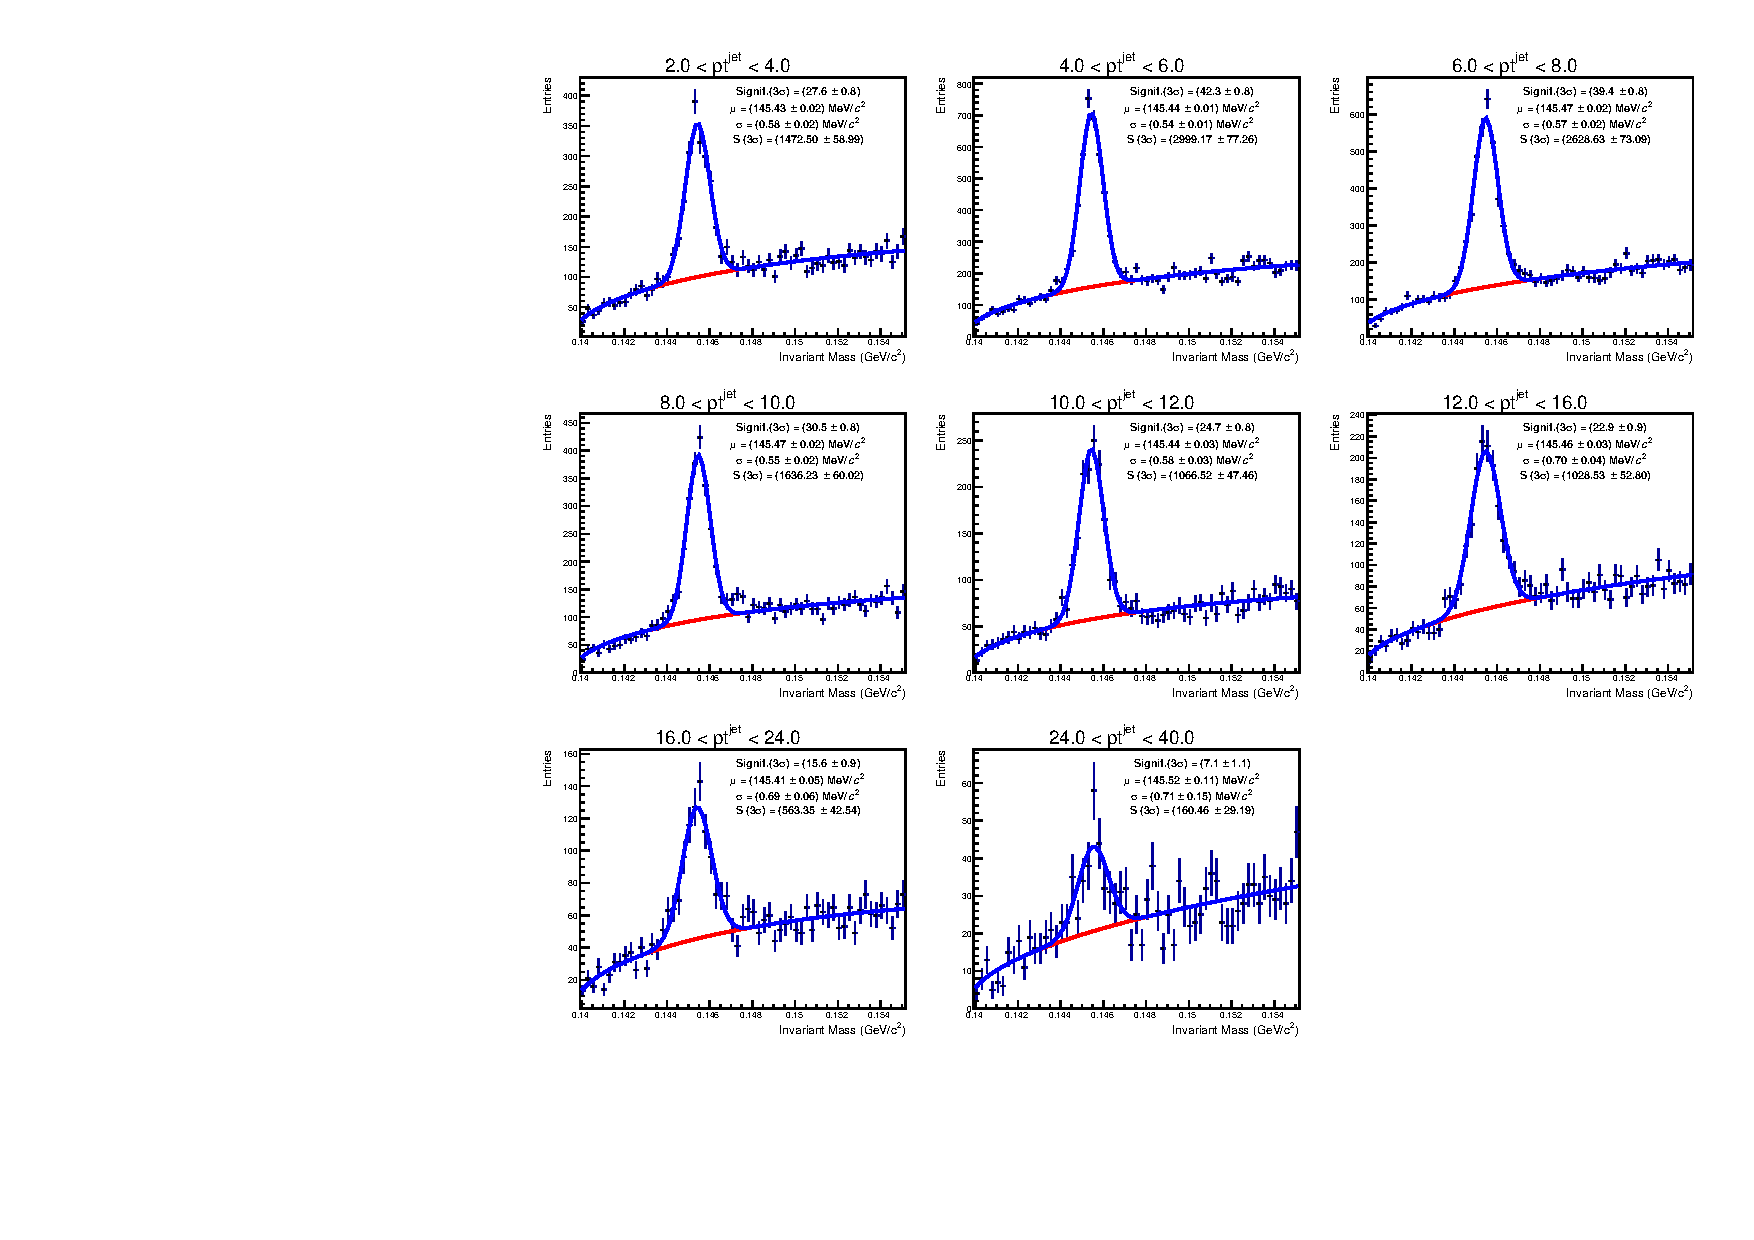
\includegraphics[width=0.9\textwidth]{pPbplots/plotsEffScale_noEff_pt3_noDetails/invMass_FASTwoSDD}
\caption{\Dstar-jet signal extraction in bins of jet transverse momentum in \pPb\ collisions at $\snn=5.02$~TeV (raw yields). D mesons are required to have $\pt>3$~\GeVc.}
\label{fig:eq_pPb_InvMass}
\end{figure}

Figure~\ref{fig:eq_pPb_RSU_raw} shows a summary of the raw signal extraction: yield, relative statistical uncertainty, signal / background ratio and significance.

\begin{figure}[bth]
\centering
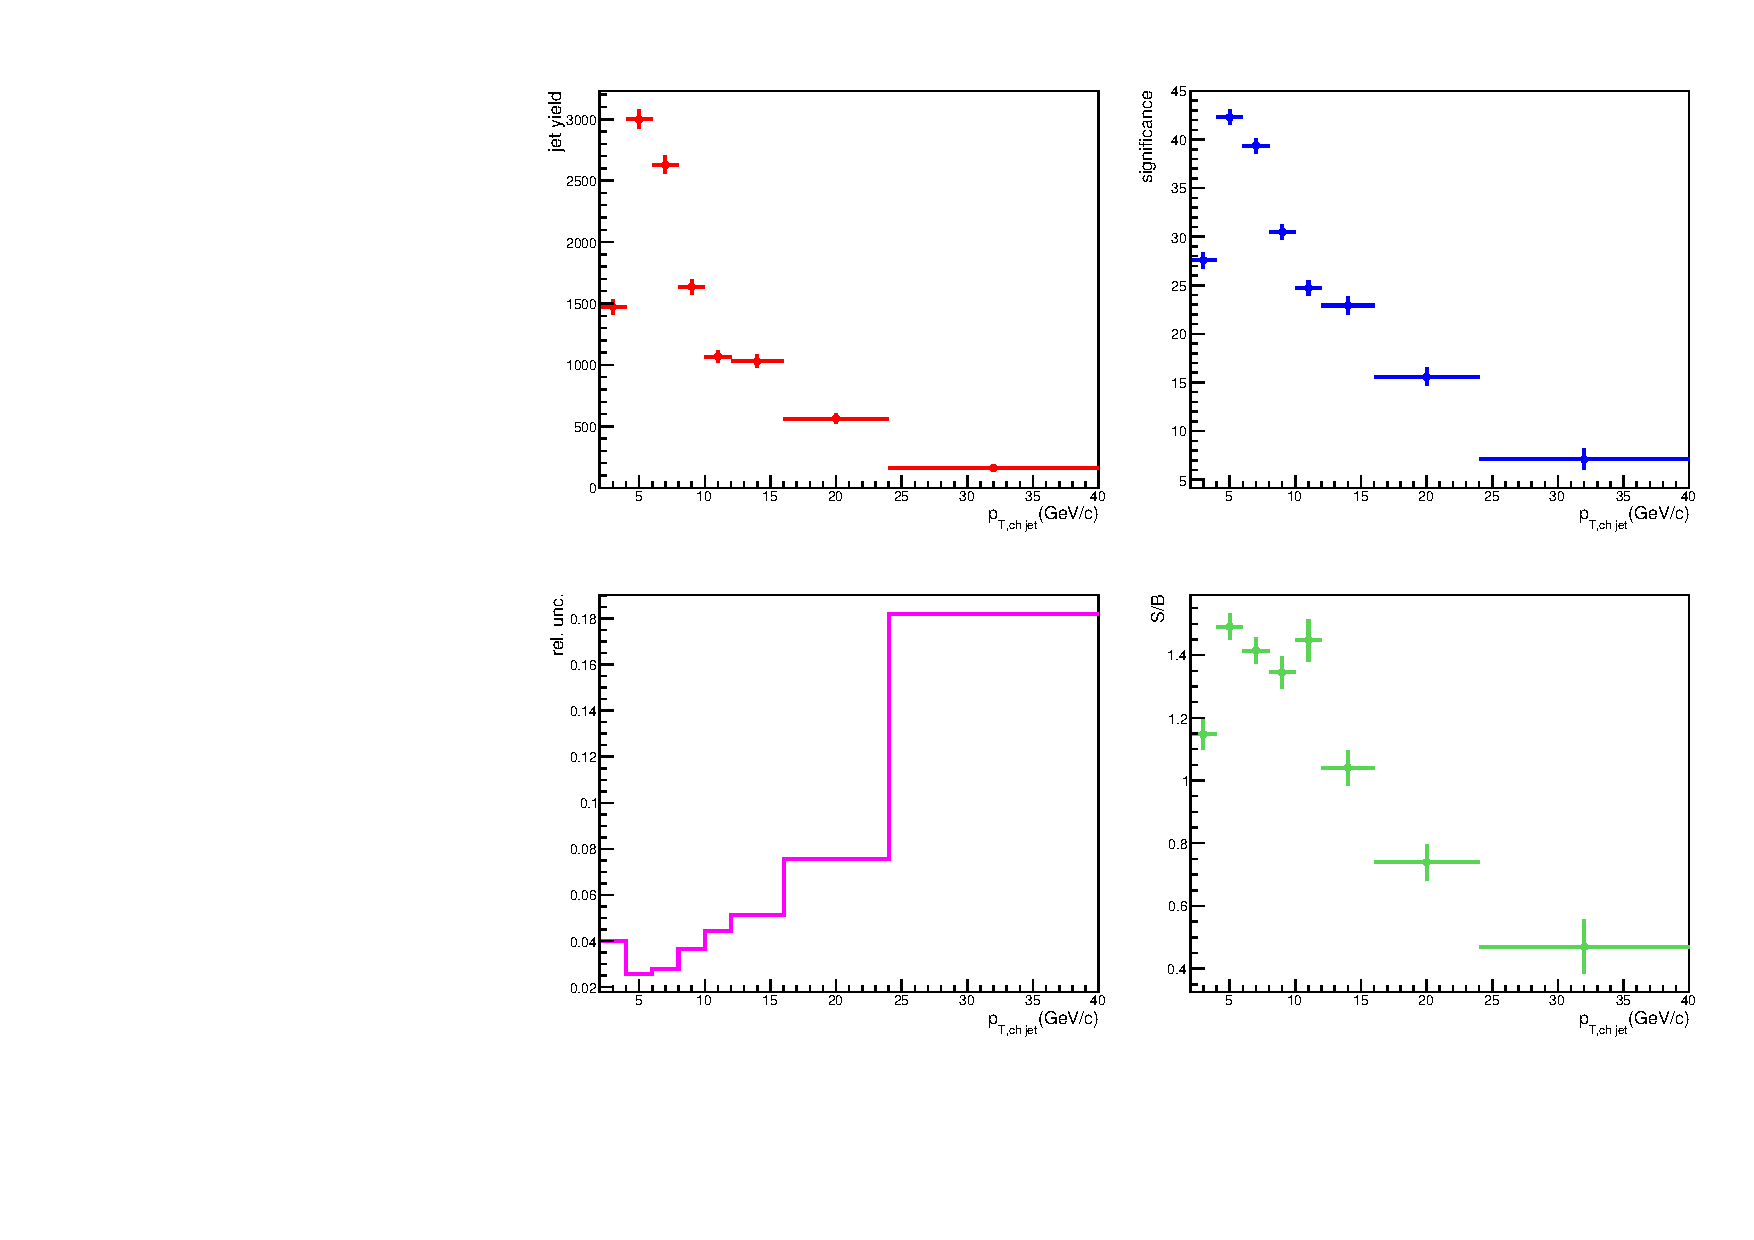
\includegraphics[width=0.7\textwidth]{pPbplots/plotsEffScale_noEff_pt3_noDetails/signalParams_FASTwoSDD}
\caption{\Dstar-jet raw signal extraction in \pPb\ collisions at $\s=5.02$~TeV for $\ptd>3$~\GeVc\ with the invariant mass fit method in bins of \ptchjet.}
\label{fig:eq_pPb_RSU_raw}
\end{figure}

The invariant mass distributions shown here are not corrected for the reconstruction efficiency. This step is discussed in Sec.~\ref{sect:sub_DmesonRecEff}.

The jet \pt\ bins are selected so that the significance of the D signal is above 5$\sigma$.
The reason of the \Dstar\ signal visible in the Fig.~\ref{fig:eq_pPb_InvMass} below \ptjet\ of 3 \GeVc\ despite the \ptd\ cut above 3 \GeVc\ is a subtraction of the jet background, as it is described in the Sec.~\ref{sBackSub}.
%The final jet \pt\ range for the \pPb\ analysis is 4 $< p_{T} < $ 40 \GeVc. 


\subsection{Side-Band Subtraction Method}
\label{sub_Bin_d_pT}

The D-meson invariant mass is analyzed for each bin of D-meson \pt. 
The D-meson candidates in the signal region are used to build a jet \pt\ distribution, which comprises both signal and background D-meson candidates.
Another jet \pt\ distribution is built using candidates with invariant mass that is between $-8\sigma$ and $-5\sigma$ from the left-hand side of the \Dstar\ peak and between $5\sigma$ and $13\sigma$ on the right-hand side.
The normalization is done using the information of the fit integrating the background function inside the signal area. This is done separately and independently for each \ptd\ bin.

The invariant mass distributions in bins of D-meson \pt\ are shown in Fig.~\ref{fig:eq_pPb_InvMass_Dbins}.

\begin{figure}[bth]
\centering
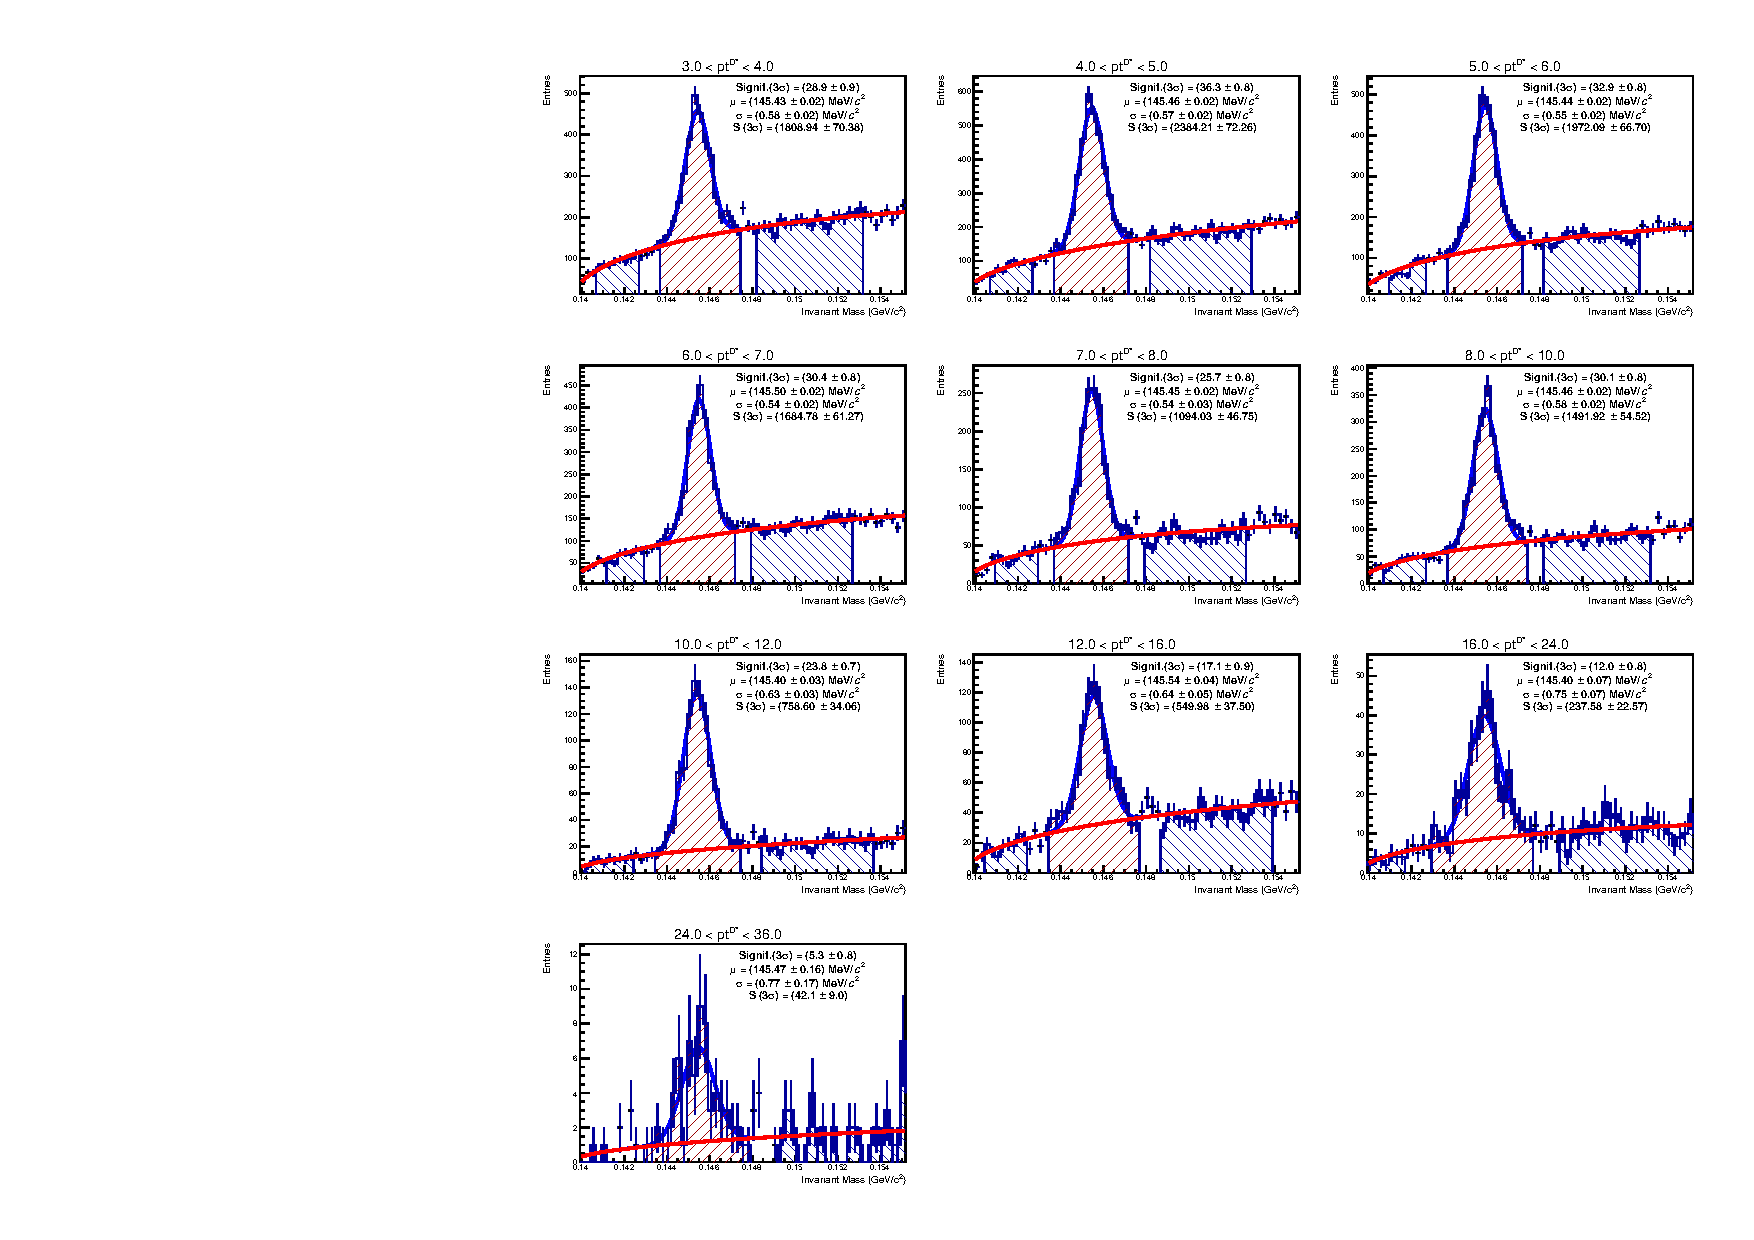
\includegraphics[width=0.9\textwidth]{pPbplots/plotsSB_noEff_pt3_noDetails/invMass_FASTwoSDD_pTD3}
\caption{\Dstar\ signal extraction in bins of D-meson transverse momentum in \pPb\ collisions at $\snn=5.02$~TeV (raw yields).}
\label{fig:eq_pPb_InvMass_Dbins}
\end{figure}

The signal region is defined as $3\sigma$ around the peak and is shown as the red shadow area in Fig.~\ref{fig:eq_pPb_InvMass_Dbins};
the background region, $5\sigma$ away from the peak mean position, is depicted as the blue area in Fig.~\ref{fig:eq_pPb_InvMass_Dbins}.

The jet \pt\ distributions are shown in Fig.~\ref{fig:eq_pPb_signBkgJet_Dbins}, along with the jet distributions for the background region. 
Then the background distributions are subtracted from the signal distributions and raw jet \pt\ distributions are obtained in each D \pt\ bin, as is it shown also in Fig.~\ref{fig:eq_pPb_signBkgJet_Dbins}.
Figure~\ref{fig:eq_pPb_signBkgJet_tot} shows the sum of the jet \pt\ distributions for \Dstar-jets\ without a correction for the D meson efficiency and rebinning.

\begin{figure}[bth]
\centering
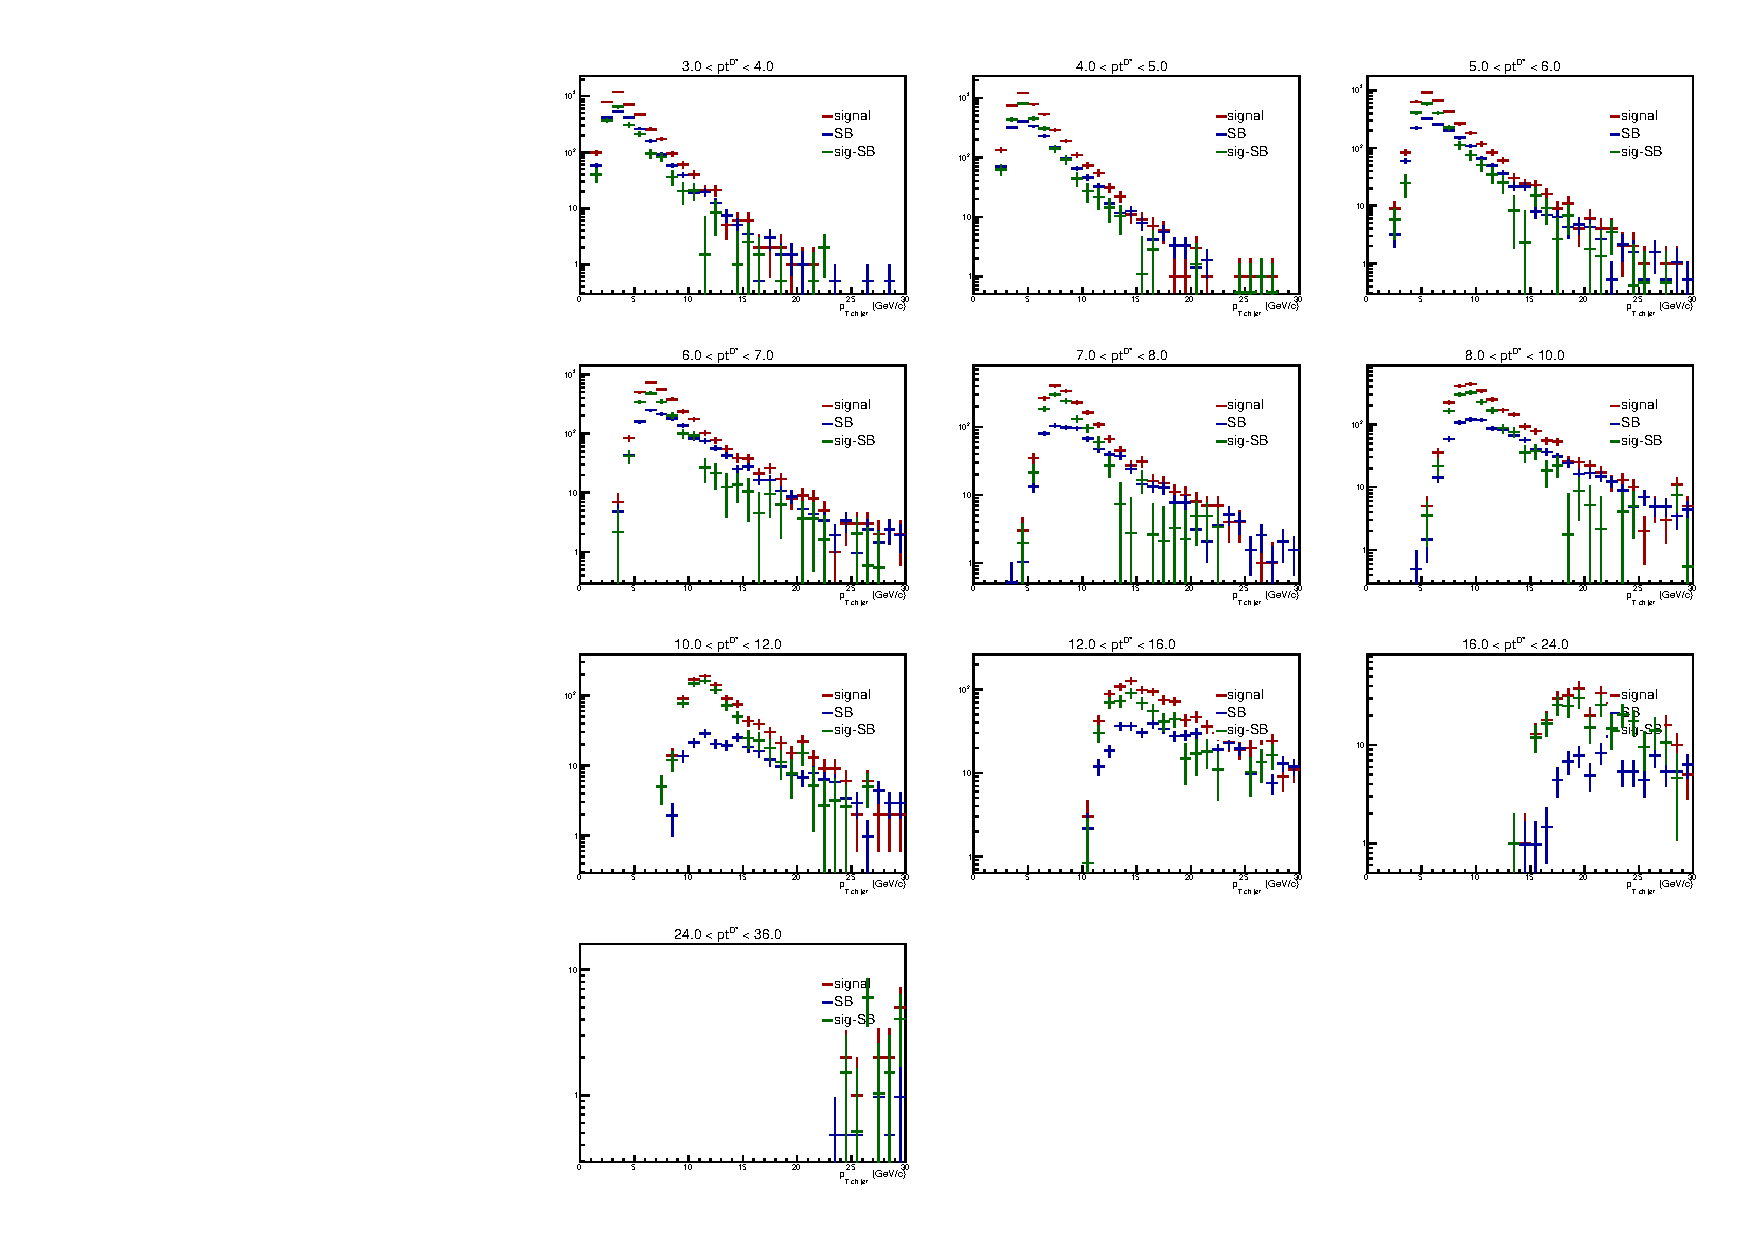
\includegraphics[width=0.9\textwidth]{pPbplots/plotsSB_noEff_pt3_noDetails/jetRawSpectrumFASTwoSDD_pTD3}
\caption{Raw jet \pt\ distributions in bins of D-meson transverse momentum in \pPb\ collisions at $\snn=5.02$~TeV.}
\label{fig:eq_pPb_signBkgJet_Dbins}
\end{figure}

\begin{figure}[bth]
\centering
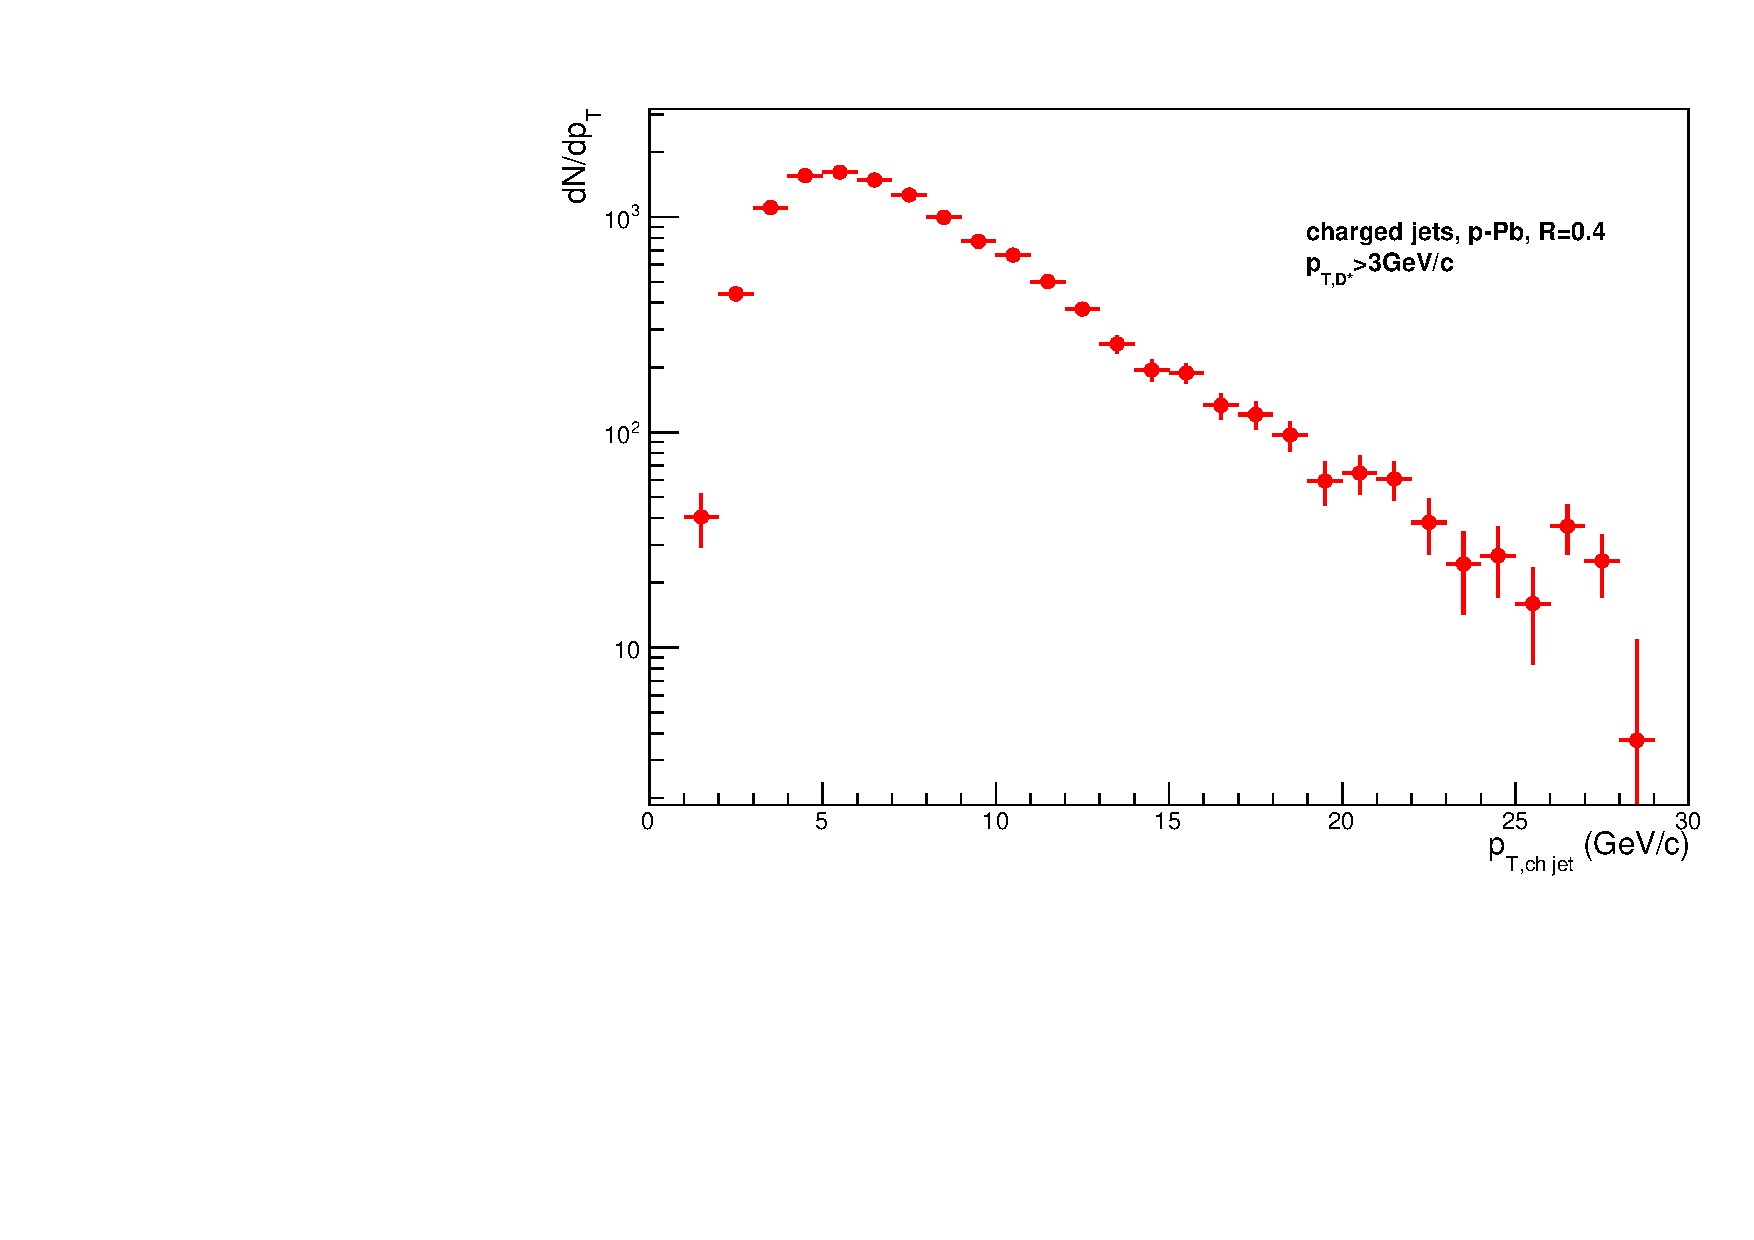
\includegraphics[width=0.5\textwidth]{pPbplots/plotsSB_noEff_pt3_noDetails/jetPtSpectrum_SB_FASTwoSDD_pTD3}
\caption{Total raw jet \pt\ distributions in \pPb\ collisions at $\snn=5.02$~TeV, obtained summing together all the \Dstar\ \pt\ bins.}
\label{fig:eq_pPb_signBkgJet_tot}
\end{figure}

Figure~\ref{fig:eq_pPb_RSU_raw_Dbins} shows a summary of the raw signal extraction:
yield, relative statistical uncertainty, signal / background ratio and significance.

\begin{figure}[bth]
\centering
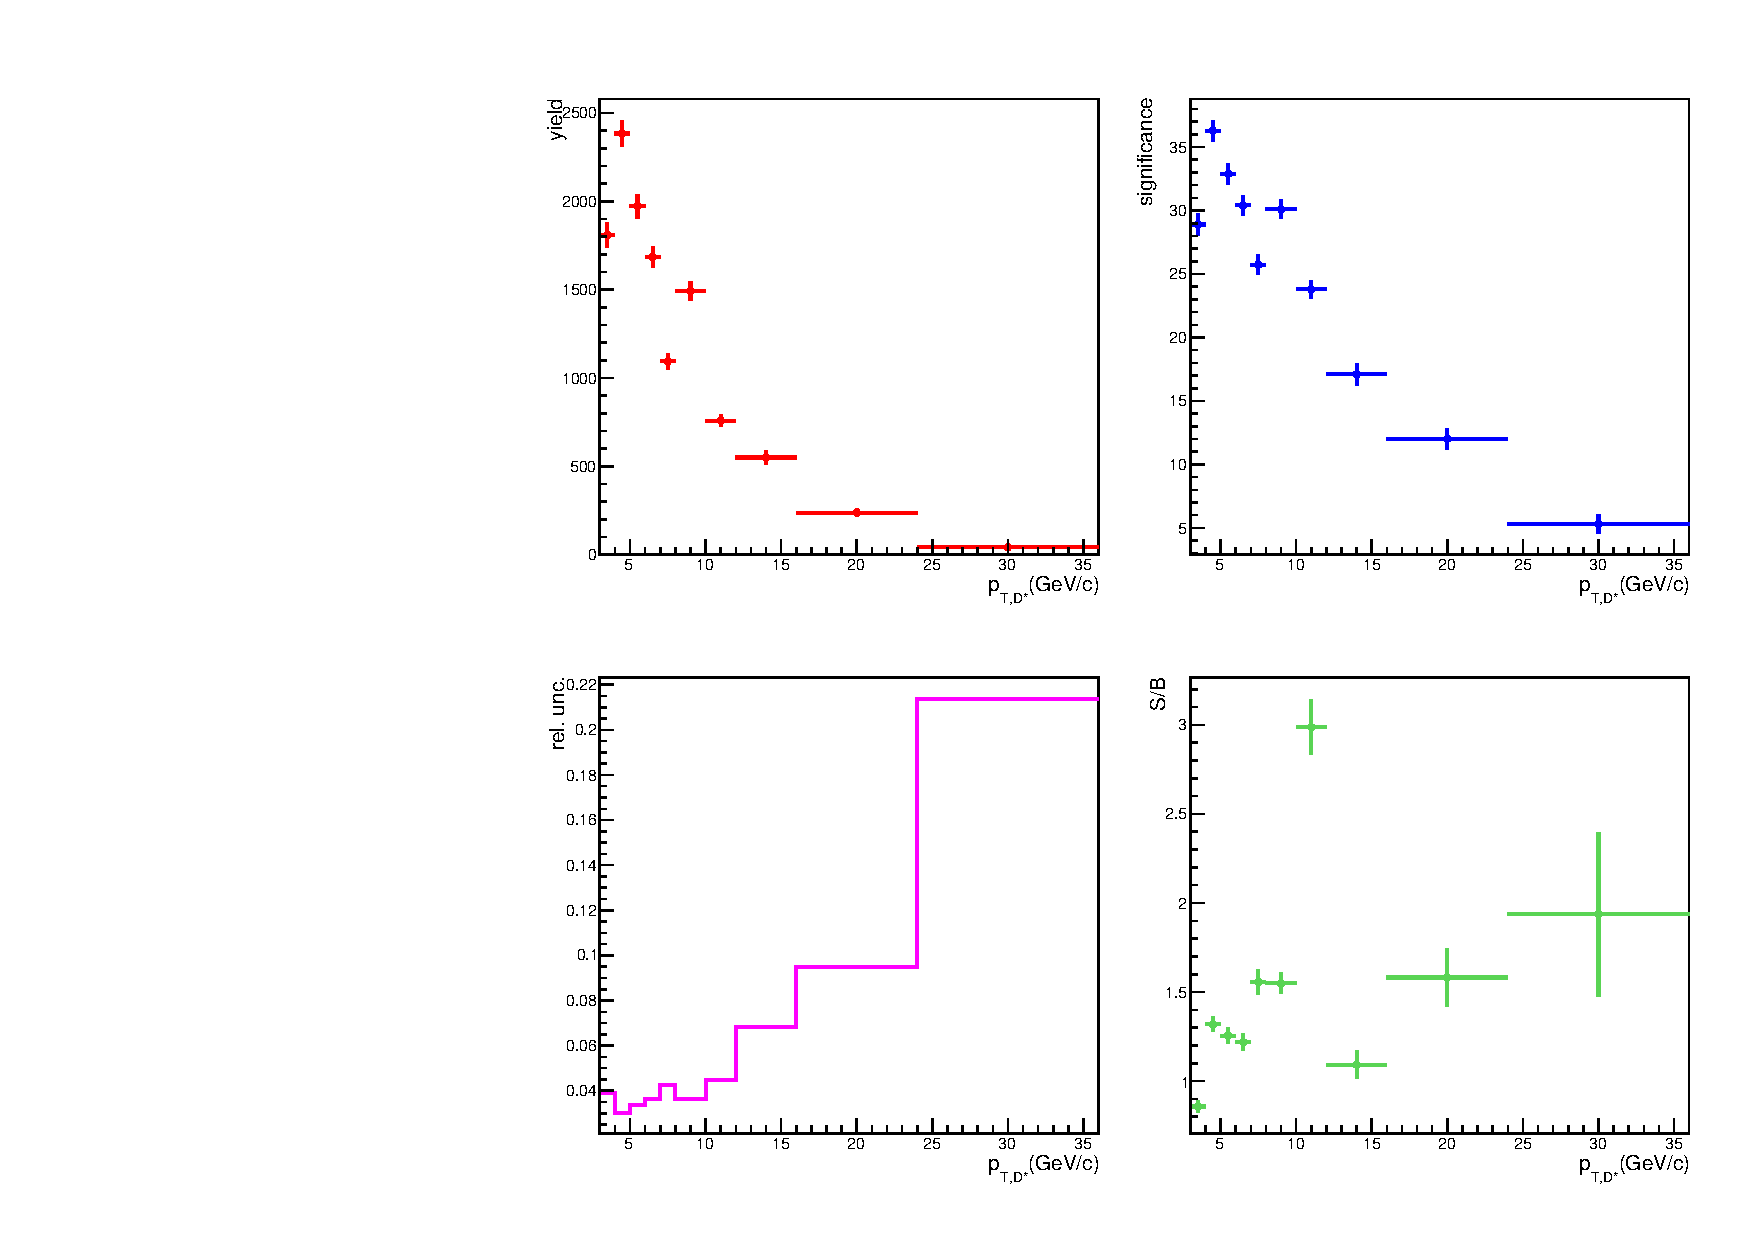
\includegraphics[width=0.7\textwidth]{pPbplots/plotsSB_noEff_pt3_noDetails/signalParams_FASTwoSDD_pTD3}
\caption{\Dstar-jet raw signal extraction in \pPb\ collisions at $\s=5.02$~TeV for $\ptd>3$~\GeVc\ with the Side Band method.}
\label{fig:eq_pPb_RSU_raw_Dbins}
\end{figure}

In order to obtain the final jet \pt\ spectrum, the distributions in each D \pt\ bin need to be corrected for the D efficiency and finally summed up.
The corrections will be discussed in Section~\ref{sect:sub_DmesonRecEff}. 

\subsection{Method Comparison}

Figure~\ref{fig:pPbCompInvMassFitSB_beforeEff} shows a comparison of the raw yields (without the D-reconstruction efficiency applied). Jets spectra are checked with two cuts on the D-meson $p_{T}$: $\ptd>2$~\GeVc and $\ptd>3$~\GeVc. Both agree with each other as it is seen in Fig.~\ref{fig:pPbCompInvMassFitSB_beforeEff}. However, it is more important to cross-check the two methods with different \ptd\ cuts after the efficiency correction is applied, as the background at low \ptd\ influences the analysis more, as it is shown later.

\begin{figure}[bth]
\centering
\begin{subfigure}[b]{0.45\textwidth}
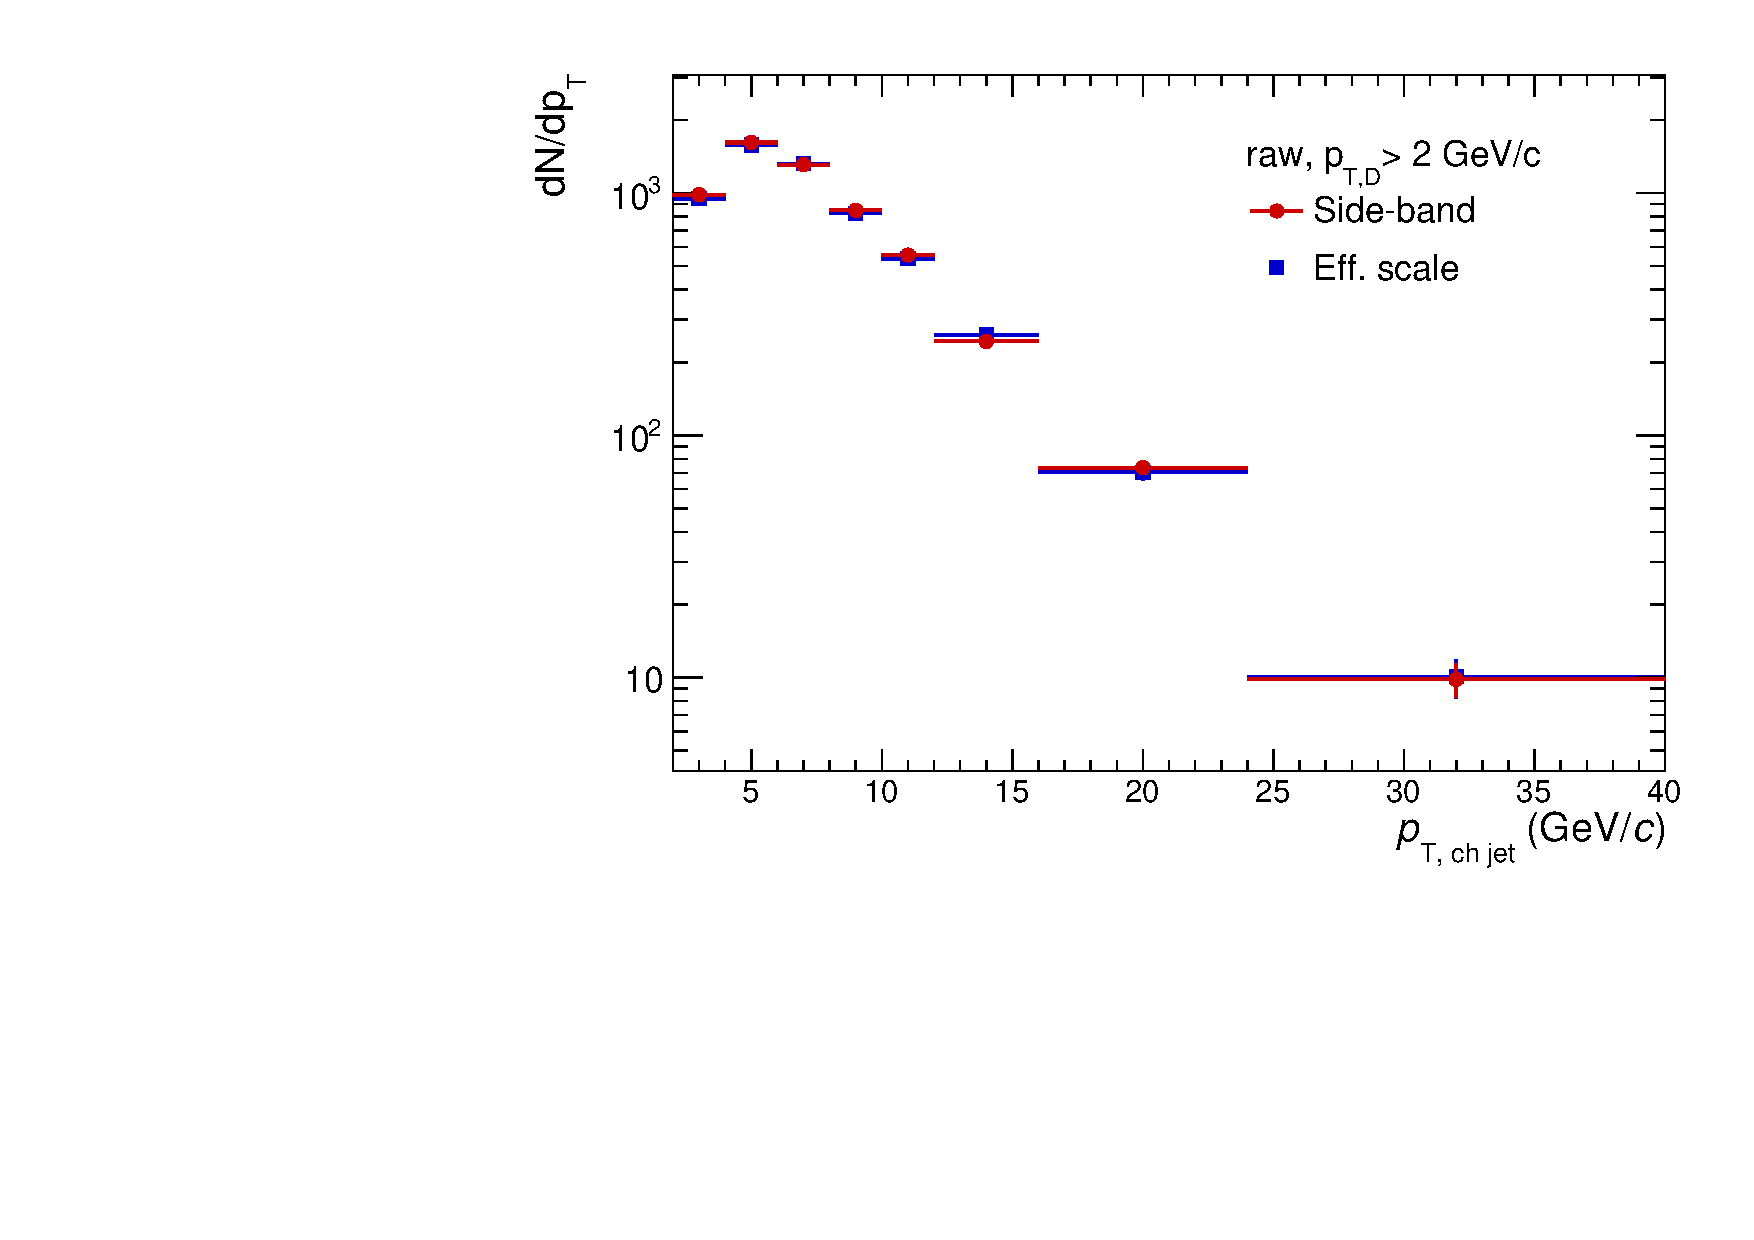
\includegraphics[width=\textwidth]{pPbplots/methodsComparison/DjetSpectra_methodComparison_FASTwoSDD_noEff_ptD2}
\caption{Yields, $\ptd>2$~\GeVc}
\end{subfigure}
\begin{subfigure}[b]{0.45\textwidth}
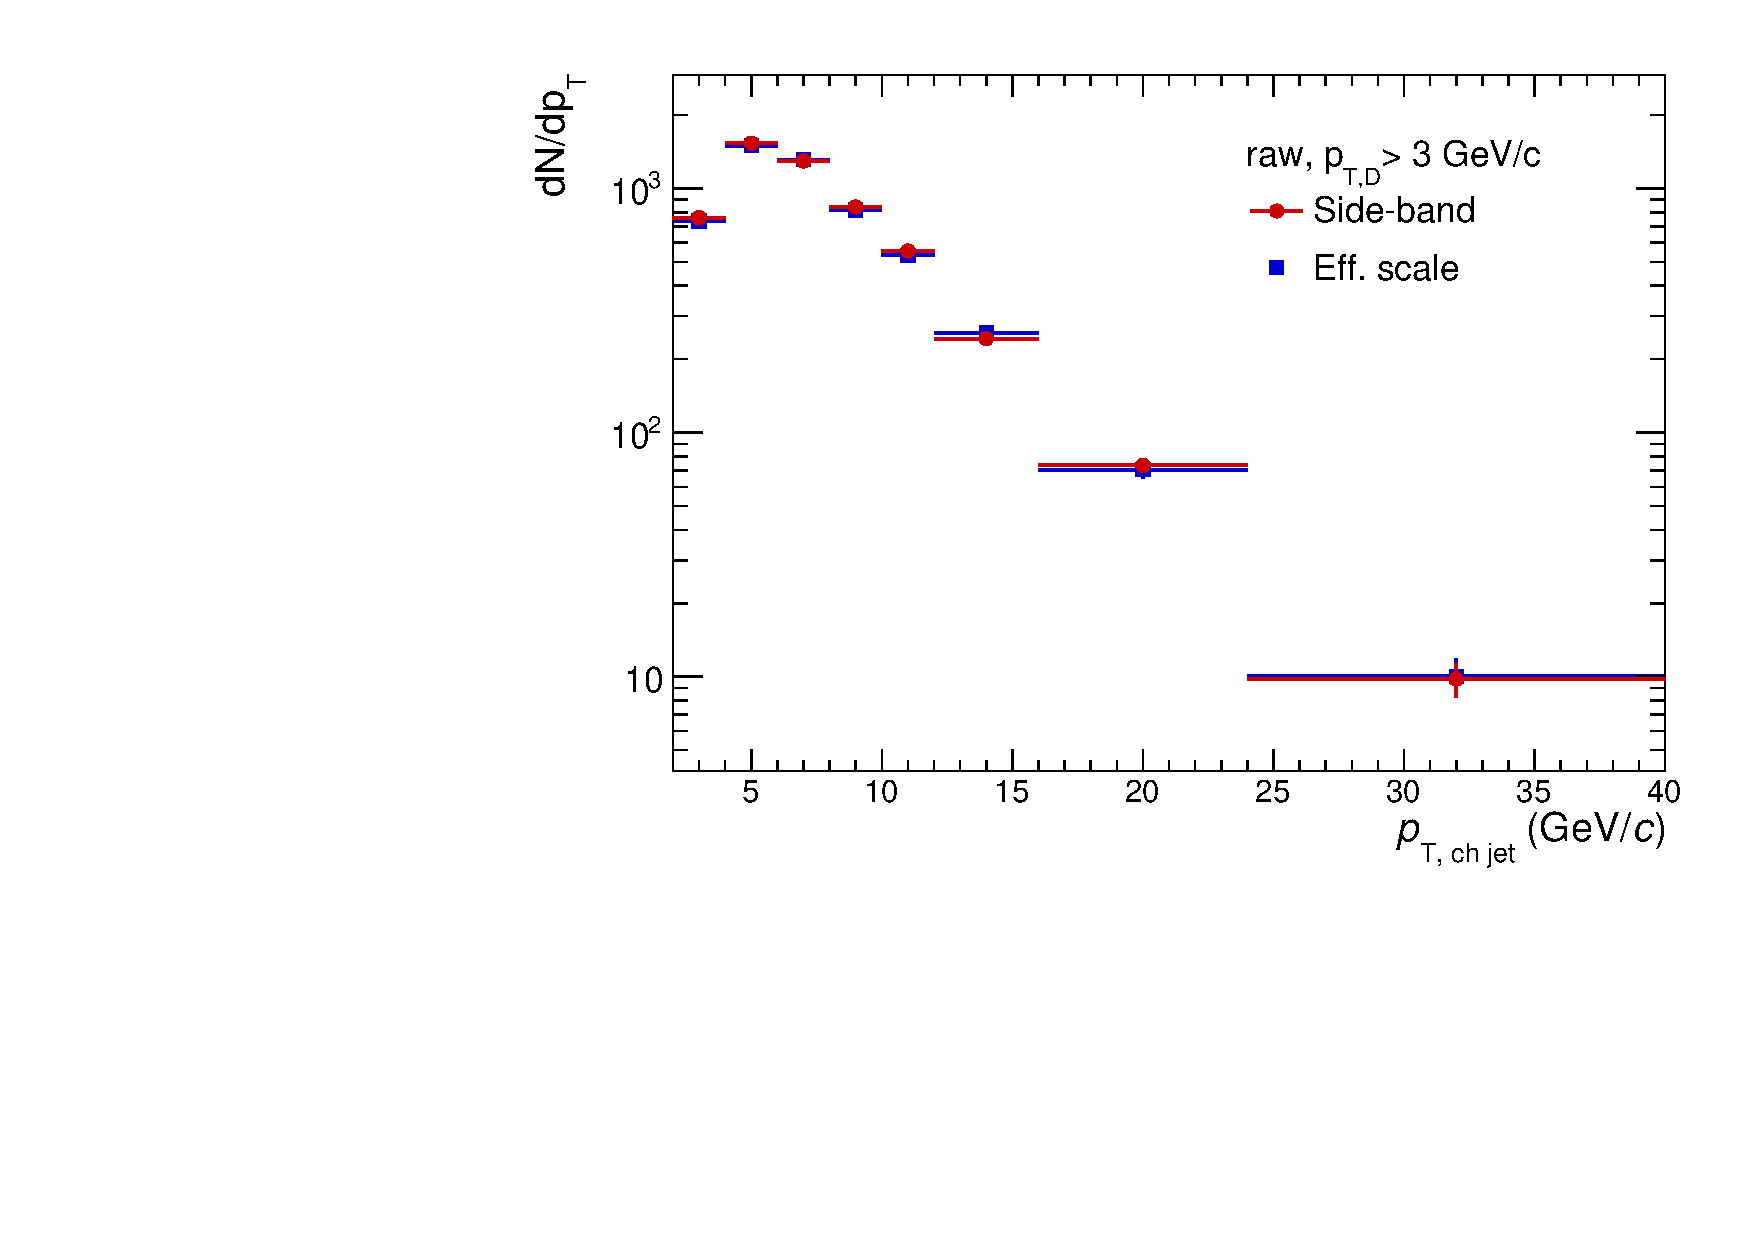
\includegraphics[width=\textwidth]{pPbplots/methodsComparison/DjetSpectra_methodComparison_FASTwoSDD_noEff_ptD3}
\caption{Yields, $\ptd>3$~\GeVc}
\end{subfigure}
\begin{subfigure}[c]{0.45\textwidth}
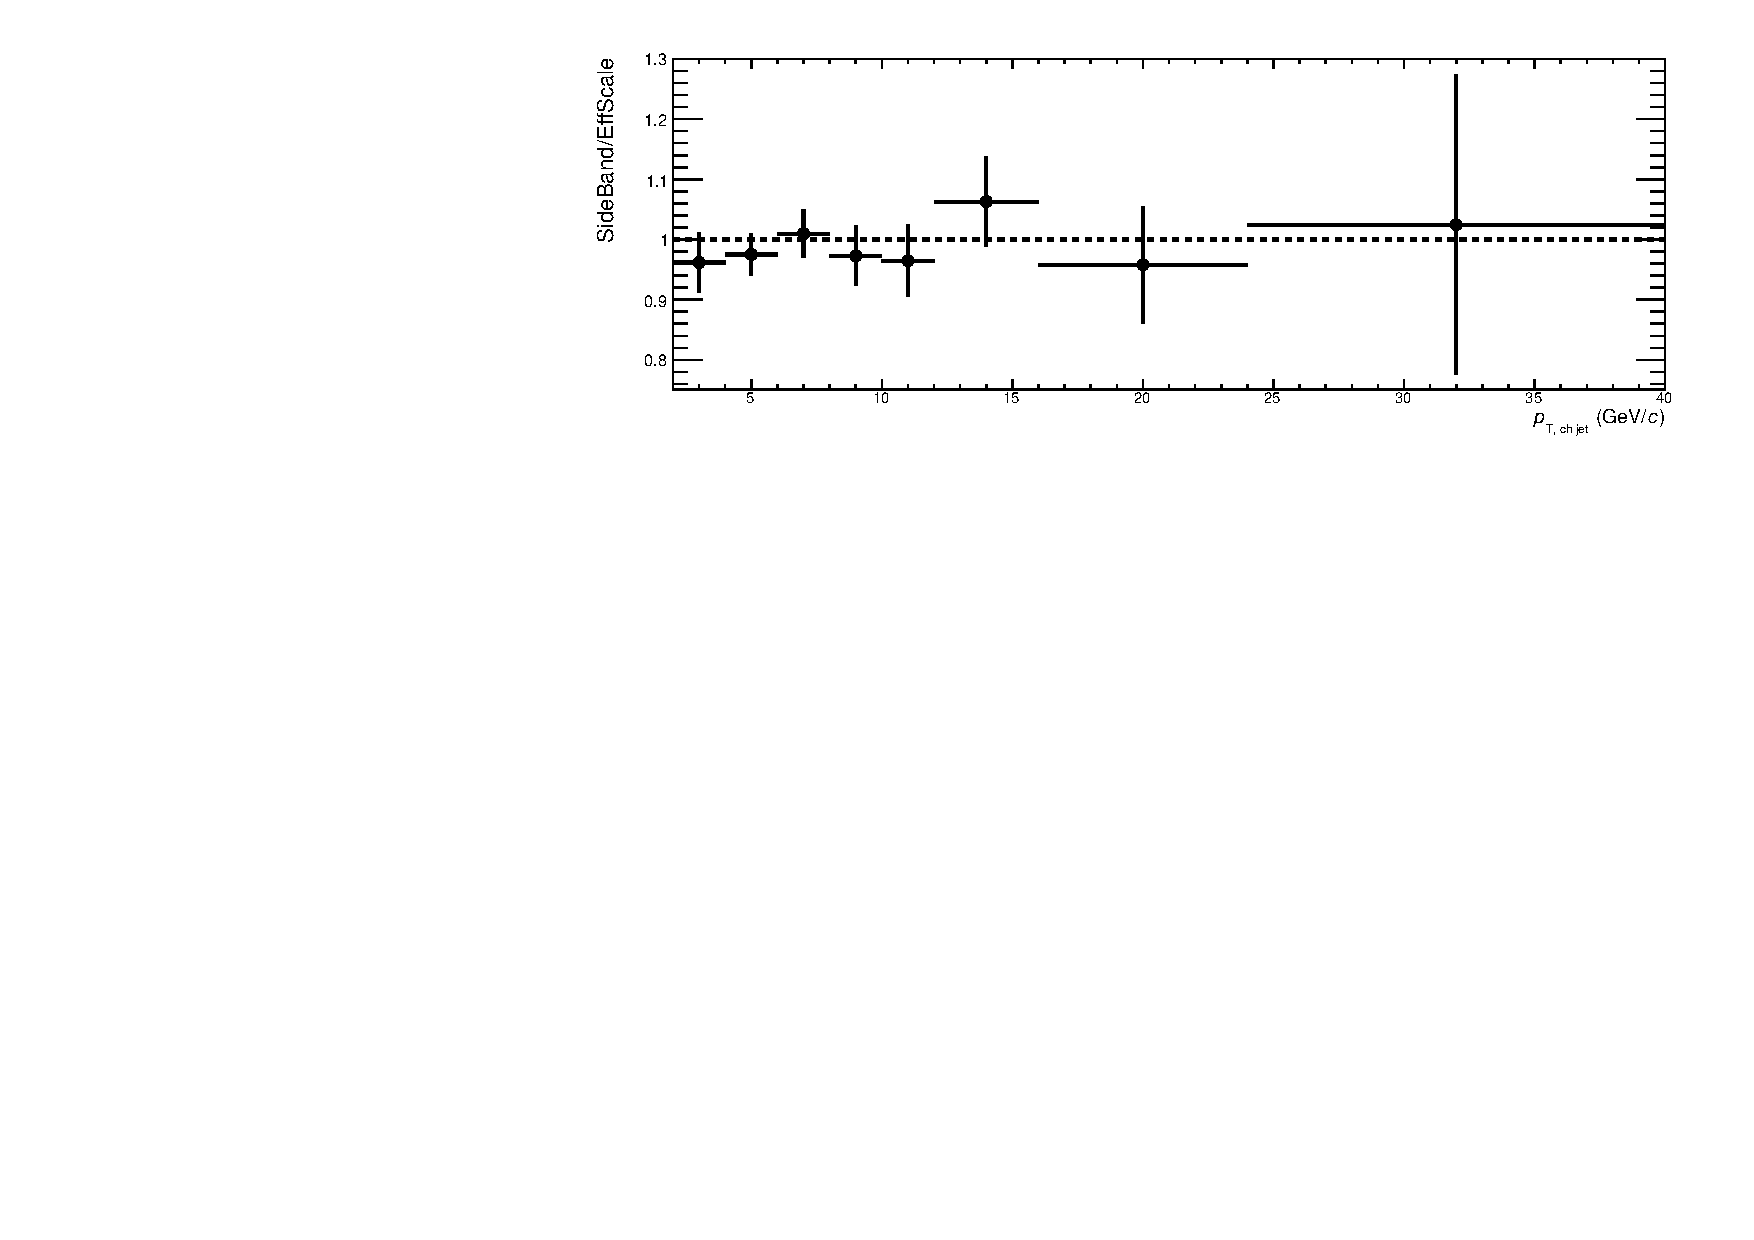
\includegraphics[width=\textwidth]{pPbplots/methodsComparison/DjetSpectraRatio_FASTwoSDD_noEff_ptD2}
\caption{Ratio, $\ptd>2$~\GeVc}
\end{subfigure}
\begin{subfigure}[d]{0.45\textwidth}
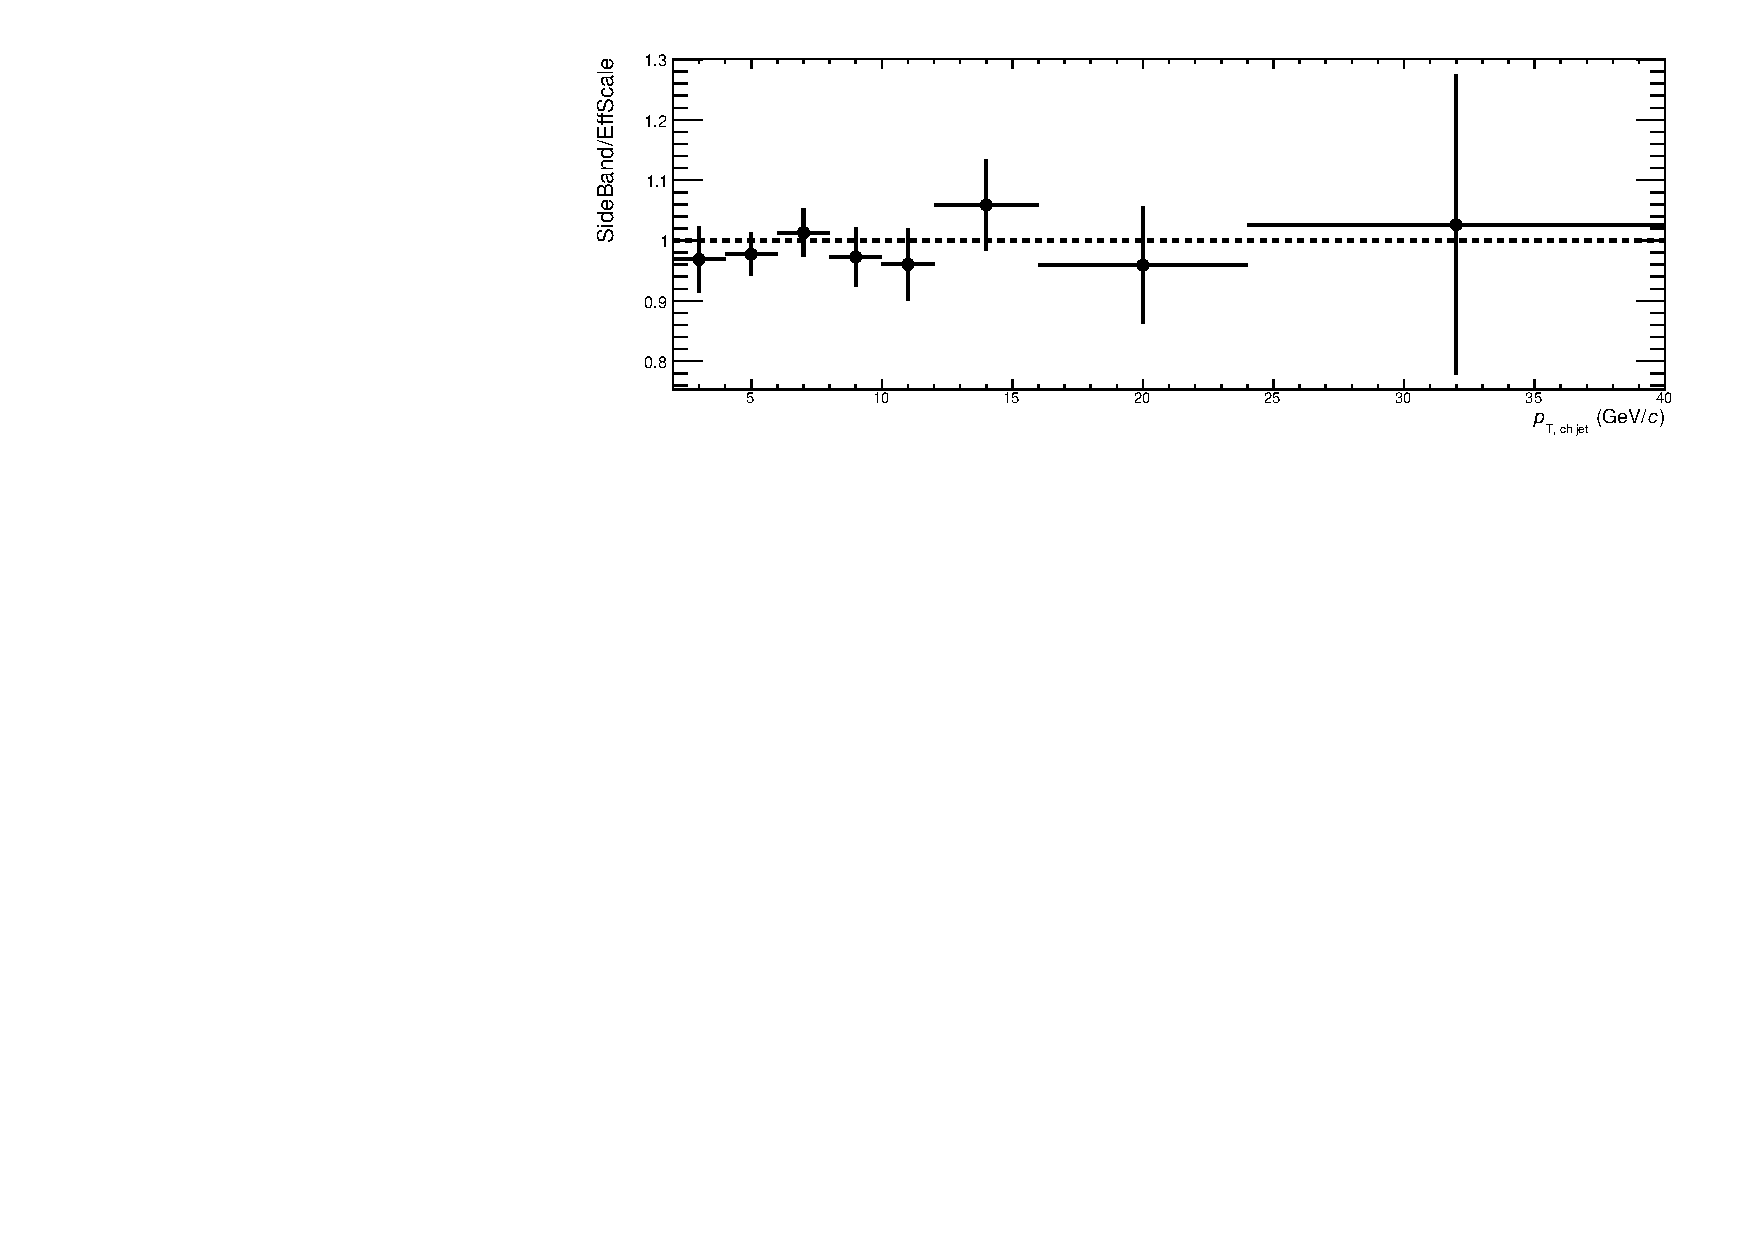
\includegraphics[width=\textwidth]{pPbplots/methodsComparison/DjetSpectraRatio_FASTwoSDD_noEff_ptD3}
\caption{Ratio, $\ptd>3$~\GeVc}
\end{subfigure}
\caption{Comparison of the raw yields obtained using the invariant mass fit method and the side band method without the efficiency correction for \Dstar-jets in \pPb\ collisions at $\s=5.02$~TeV with $\ptd>2$~\GeVc (left) and $\ptd>3$~\GeVc (right).}
\label{fig:pPbCompInvMassFitSB_beforeEff}
\end{figure}

%%%%%%%%%%%%%%%%%%%%%%%%%%%%%%%%%%%%%%%%%%%%%%%%%%%%%%%%%%%%%%%%%%%%%%
%%%%%%%%%%%%%%%%%%%%%%%%%%%%%%%%%%%%%%%%%%%%%%%%%%%%%%%%%%%%%%%%%%%%%%
%%%%%%%%%%%%%%%%%%%%%%%%%%%%           EFFICIENCY            %%%%%%%%%%%%%%%%%%%%%%%%%%%%
%%%%%%%%%%%%%%%%%%%%%%%%%%%%%%%%%%%%%%%%%%%%%%%%%%%%%%%%%%%%%%%%%%%%%%
%%%%%%%%%%%%%%%%%%%%%%%%%%%%%%%%%%%%%%%%%%%%%%%%%%%%%%%%%%%%%%%%%%%%%%

\section{Efficiency Correction Procedure}

\subsection{Reconstruction Efficiency}
\label{sect:sub_DmesonRecEff}
The efficiency and acceptance (${\rm Acc} \times \epsilon$) were calculated using Monte Carlo PYTHIA6+GEANT3 simulations anchored to the data.

The efficiency is taken as the ratio of the \ptd\ spectra of the D-tagged generator-level jets for which a matched
D-tagged detector-level jet was found over all the generated D-tagged jets.
For the detector-level jets, the D meson is required to be within the standard fiducial rapidity cuts.
Jets are further requested to have $|\eta_{\rm jet}| < 0.9 - R$, both at generator and detector levels.


\begin{figure}[bth]
\centering
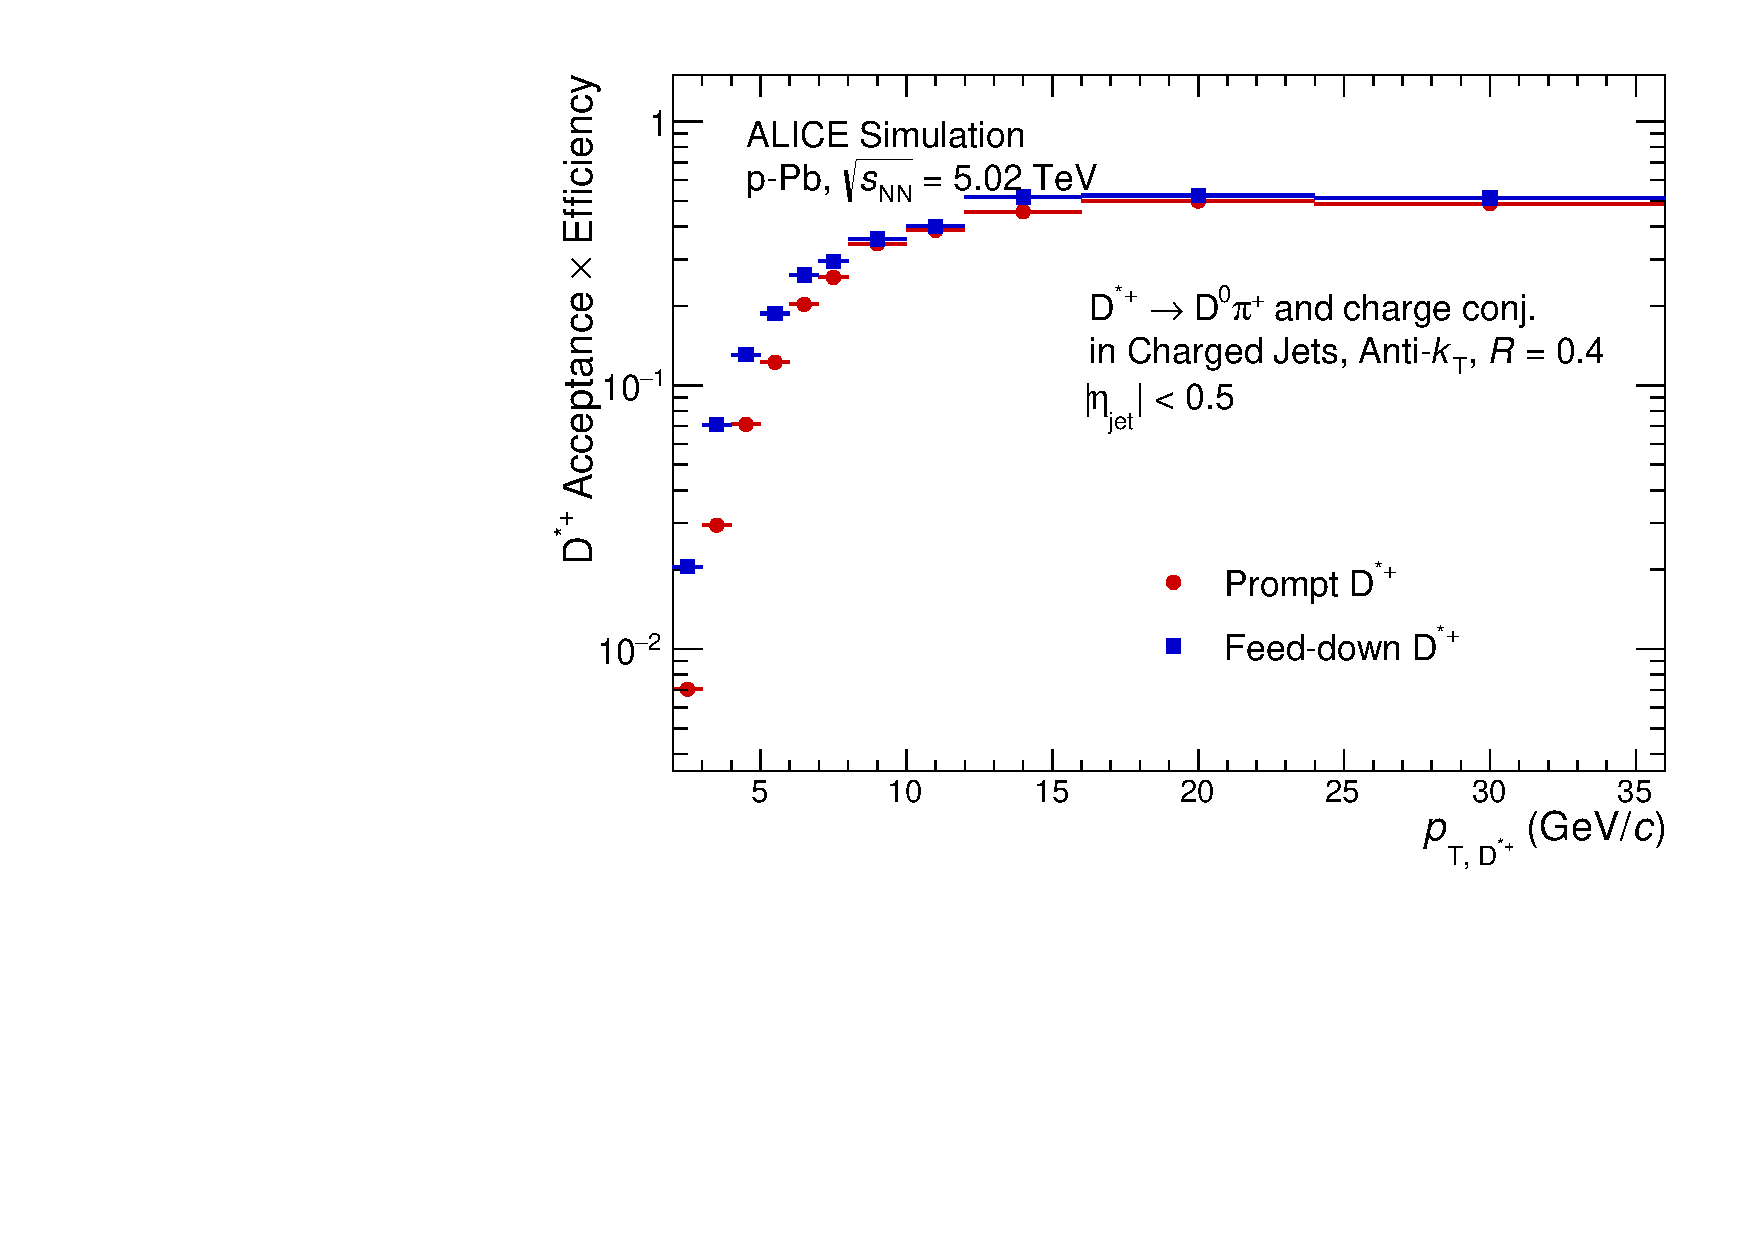
\includegraphics[width=0.6\textwidth]{pPbplots/DjetEff_Sim_log}
\caption{\Dstar\  reconstruction efficiency in \pPb\ collisions at $\snn=5.02$~TeV, for prompt D* in red and non-prompt in blue.}
\label{eq_pPb_DrecEff}
\end{figure}

Figure~\ref{eq_pPb_DrecEff} shows the \Dstar\ reconstruction efficiency as a function of \ptd\, for prompt and non-prompt \Dstar. The efficiency depends strongly on \ptd\ because of the topological cuts that are relaxed at higher momenta where the combinatorial background is smaller. 

%However a very weak or no dependence on \ptchjet\ is observed for $5<\ptchjet<30$~\GeVc. From the ratios of the efficiencies in \ptchjet\ bins over the entire range, shown in Fig.~\ref{fig:eq_pp_DrecEff_ptd_ptjet} one can appreciate a hint of a small deviation, on the order of 10-20\%, for low momentum \Dzero\ (\ptd~$<5$~\GeVc) in high momentum jets. However this deviation is not statistically significant, and affects a very small fraction of the D-meson candidates.

\subsection{Efficiency-Corrected Yields}

As discussed in the previous Section, the D-meson reconstruction efficiency shows a strong dependence on \ptd (but has very weak or no dependence on \ptjet).
Therefore, in order to reduce the dependence on the Monte Carlo simulation for what concerns jet fragmentation and momentum spectral shape,
the efficiency should be applied as a function of the D-meson momentum. In fact, each bin of \ptjet\ has contributions from D mesons with very different \ptd,
which have different efficiencies.

The efficiency-rescaling procedure of the invariant mass distribution $M(\ptjet,\ptd)$ was implemented according to the following formula:
\begin{equation}
M(\ptjet) = \displaystyle\sum_{\ptd}\frac{M(\ptjet,\ptd)}{({\rm Acc} \times \epsilon)_{\ptd}}.
\end{equation}

Figure~\ref{fig:eq_pPb_InvMass_corrDrec} shows the invariant mass distributions for different ranges of \ptchjet, after the efficiency reweighing procedure.
%This process can increase the relative statistical uncertainty due to the large weight assigned to low-\pt\ D mesons (low reconstruction efficiency). 

\begin{figure}[bth]
\centering
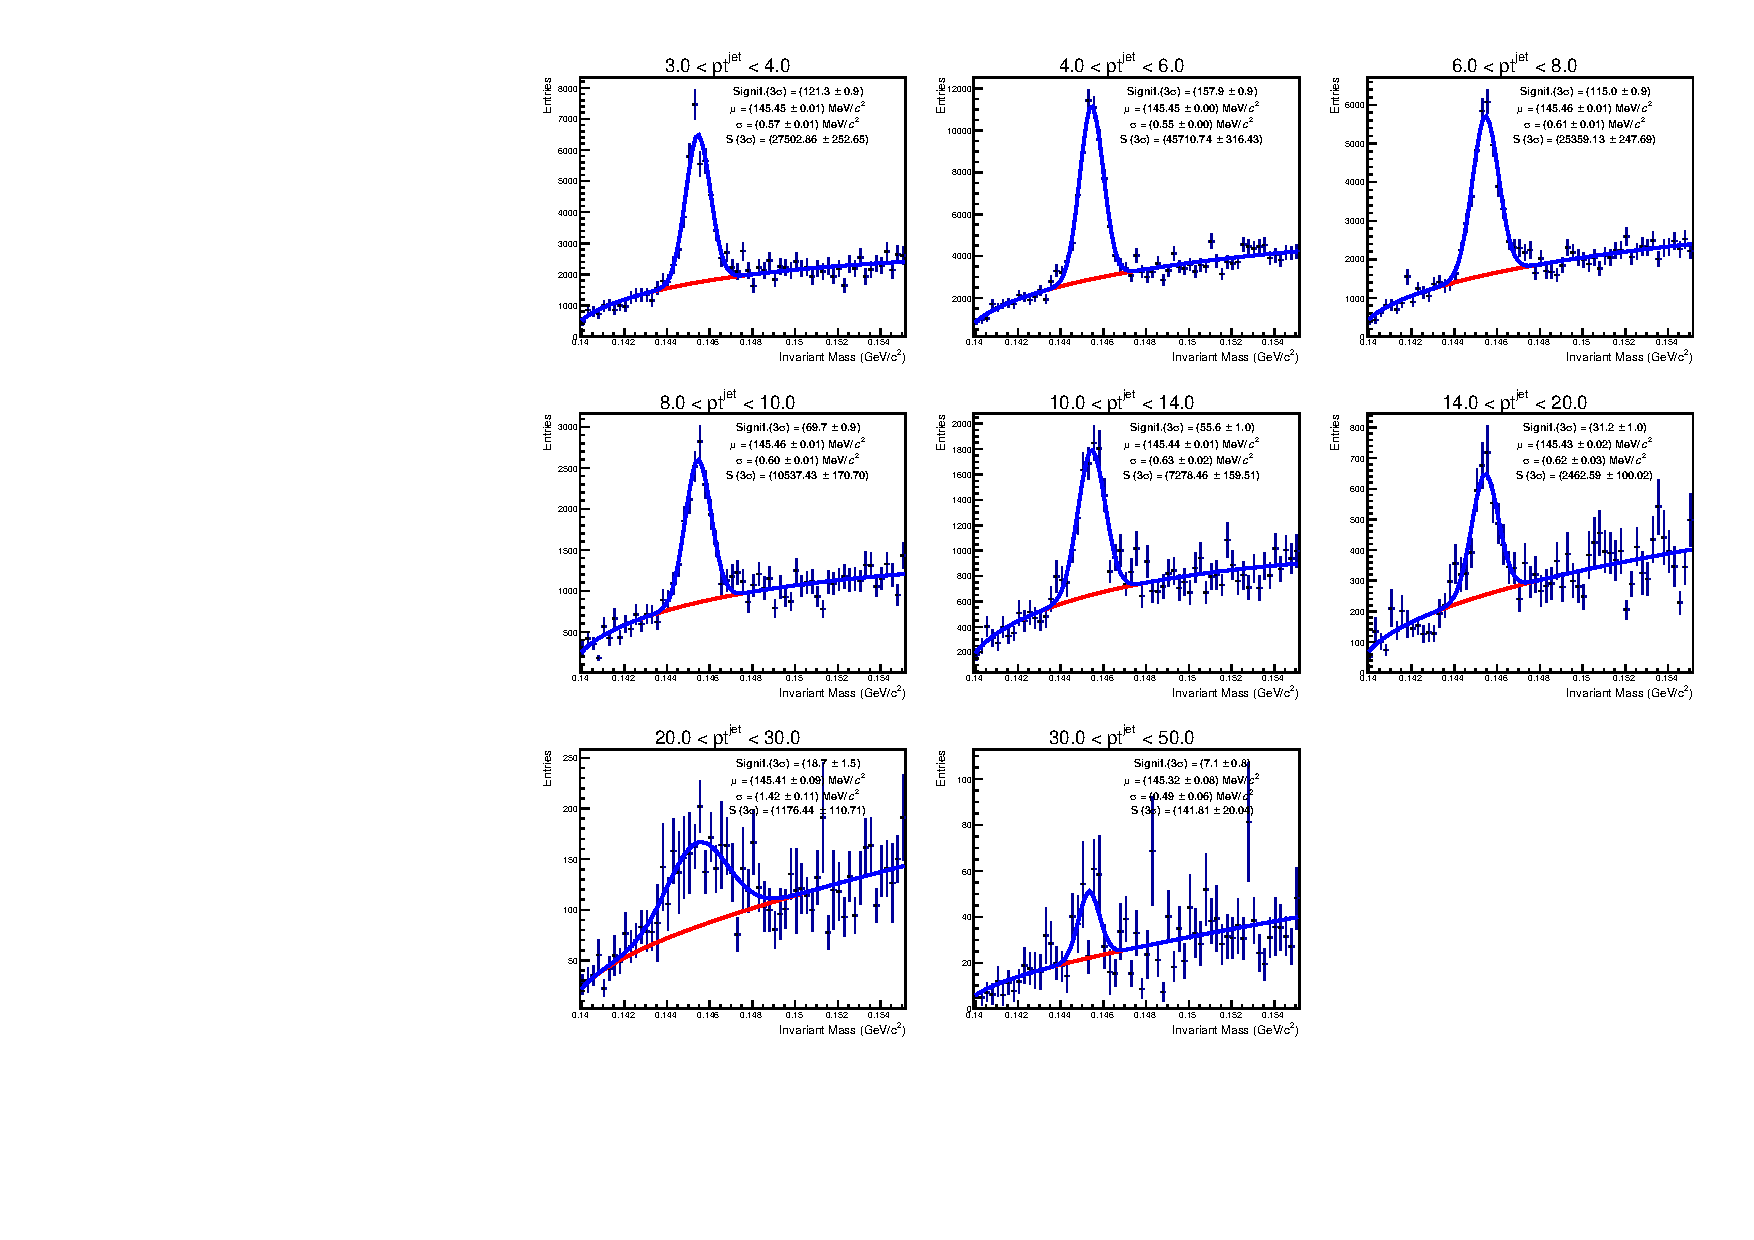
\includegraphics[width=0.9\textwidth]{pPbplots/plotsEffScale_pt3_noDetails/invMass_FASTwoSDD}
\caption{\Dstar\ signal extraction in bins of jet transverse momentum in \pPb\ collisions at $\snn=5.02$~TeV. D mesons are required to have $\ptd>3$~\GeVc.
Each candidate is weighted by the inverse of the reconstruction efficiency, which depends on its \ptd.}
\label{fig:eq_pPb_InvMass_corrDrec}
\end{figure}

%Figure~\ref{fig:eq_pPb_RSU_raw_corrDrec} shows the yield and relative statistical uncertainties of the reconstructed D-tagged jets with the efficiency weighting with the invariant mass fit method. A comparison with ~\ref{fig:eq_pPb_RSU_raw} shows  that the relative statistical uncertainties are increased as a result of the efficiency weighting.

In the side-band method the efficiency is applied by rescaling by 1/(${\rm Acc} \times \epsilon$) the jet \pt\ spectra in each D-meson \pt\ bin shown in 
Fig.~\ref{fig:eq_pPb_signBkgJet_Dbins}. 
The background subtracted distributions are summed up to obtain the corrected jet \pt\ spectrum. The efficiency corrected spectrum is shown in Fig.~\ref{}

\begin{figure}[bth]
\centering
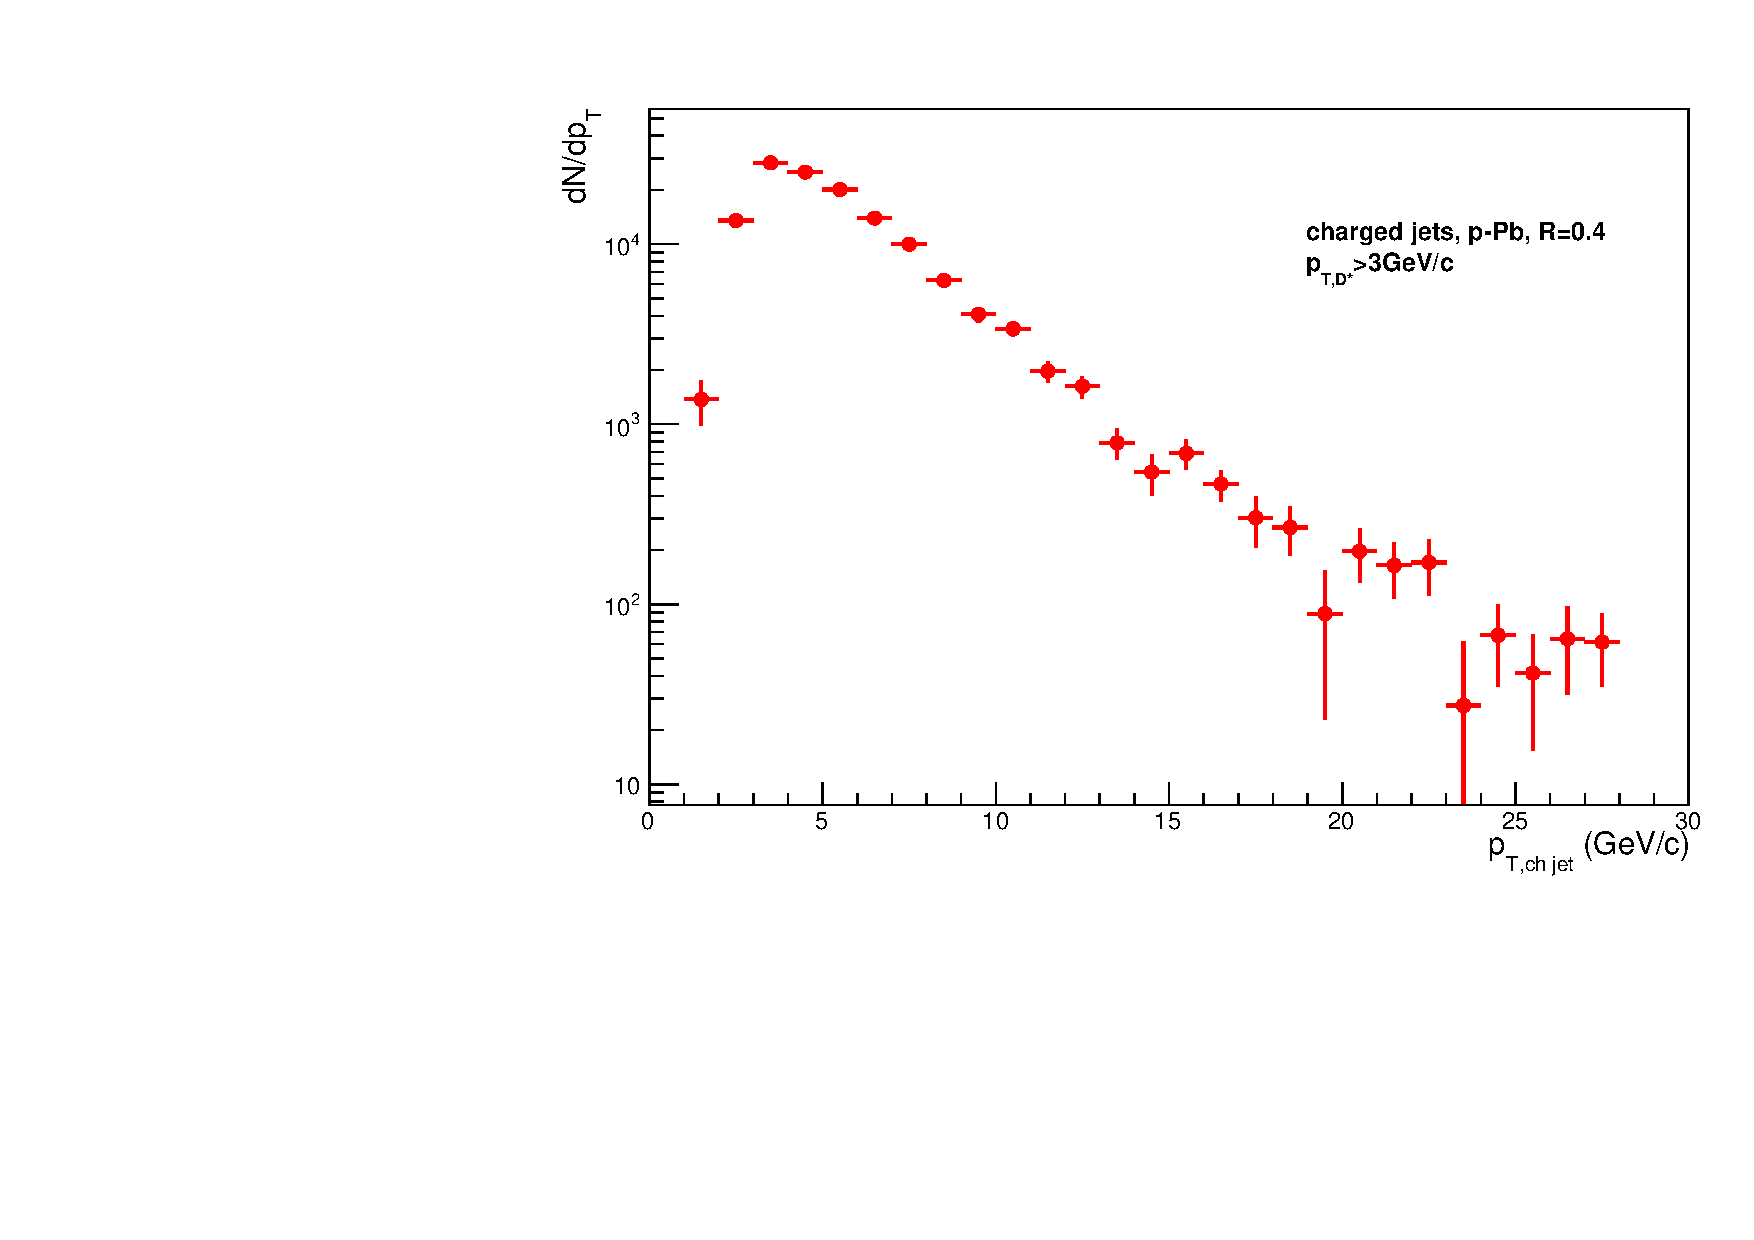
\includegraphics[width=0.6\textwidth]{pPbplots/plotsSB_pt3_noDetails/jetPtSpectrum_SB_FASTwoSDD_pTD3}
\caption{Efficiency corrected \Dstar-jets yield obtained for the Side-Band subtraction method in \pPb\ collisions at $\snn=5.02$~TeV. D mesons are required to have $\ptd>3$~\GeVc.}
\label{fig:eq_pPb_InvMass_corrDrec}
\end{figure}

The efficiency corrected jet $p_{T}$ spectra for both methods with the same binning are shown below.

\subsection{Method Comparison (Efficiency-Corrected Yields)}

Figure~\ref{fig:JetPt_pPb_corrDrec} shows a comparison of the efficiency-corrected yields obtained using the invariant mass method and the side band method
for \Dstar-jets with $\ptd>2$~\GeVc\ and $\ptd>3$~\GeVc. 
As mentioned before, the invariant mass method is sensitive to weighing with low efficiency, low $p_{T}$ D* mesons. Therefore, discrepancies for higher \ptjet\ ranges between two methods are visible with $\ptd>2$~\GeVc\ cut. With $\ptd>3$~\GeVc\ cut the two methods agree very well with each other within the statistical uncertainties.
$\ptd>3$~\GeVc\ cut reduces also uncertainties on the jet spectra for higher \ptjet. Figure~\ref{fig:JetPt_pPb_SBUnc} shows relative statistical uncertainties for the Side-Band subtraction method with $\ptd>3$~\GeVc.

F%igure~\ref{fig:JetPt_pPb_SBUnc} shows relative statistical uncertanties for the Side-Band subtraction method with $\ptd>2$~\GeVc\ and $\ptd>3$~\GeVc; $\ptd>3$~\GeVc\ cut reduces also uncertainties on the jet spectra for higher \ptjet. 

\begin{figure}[bth]
\centering
\begin{subfigure}[b]{0.45\textwidth}
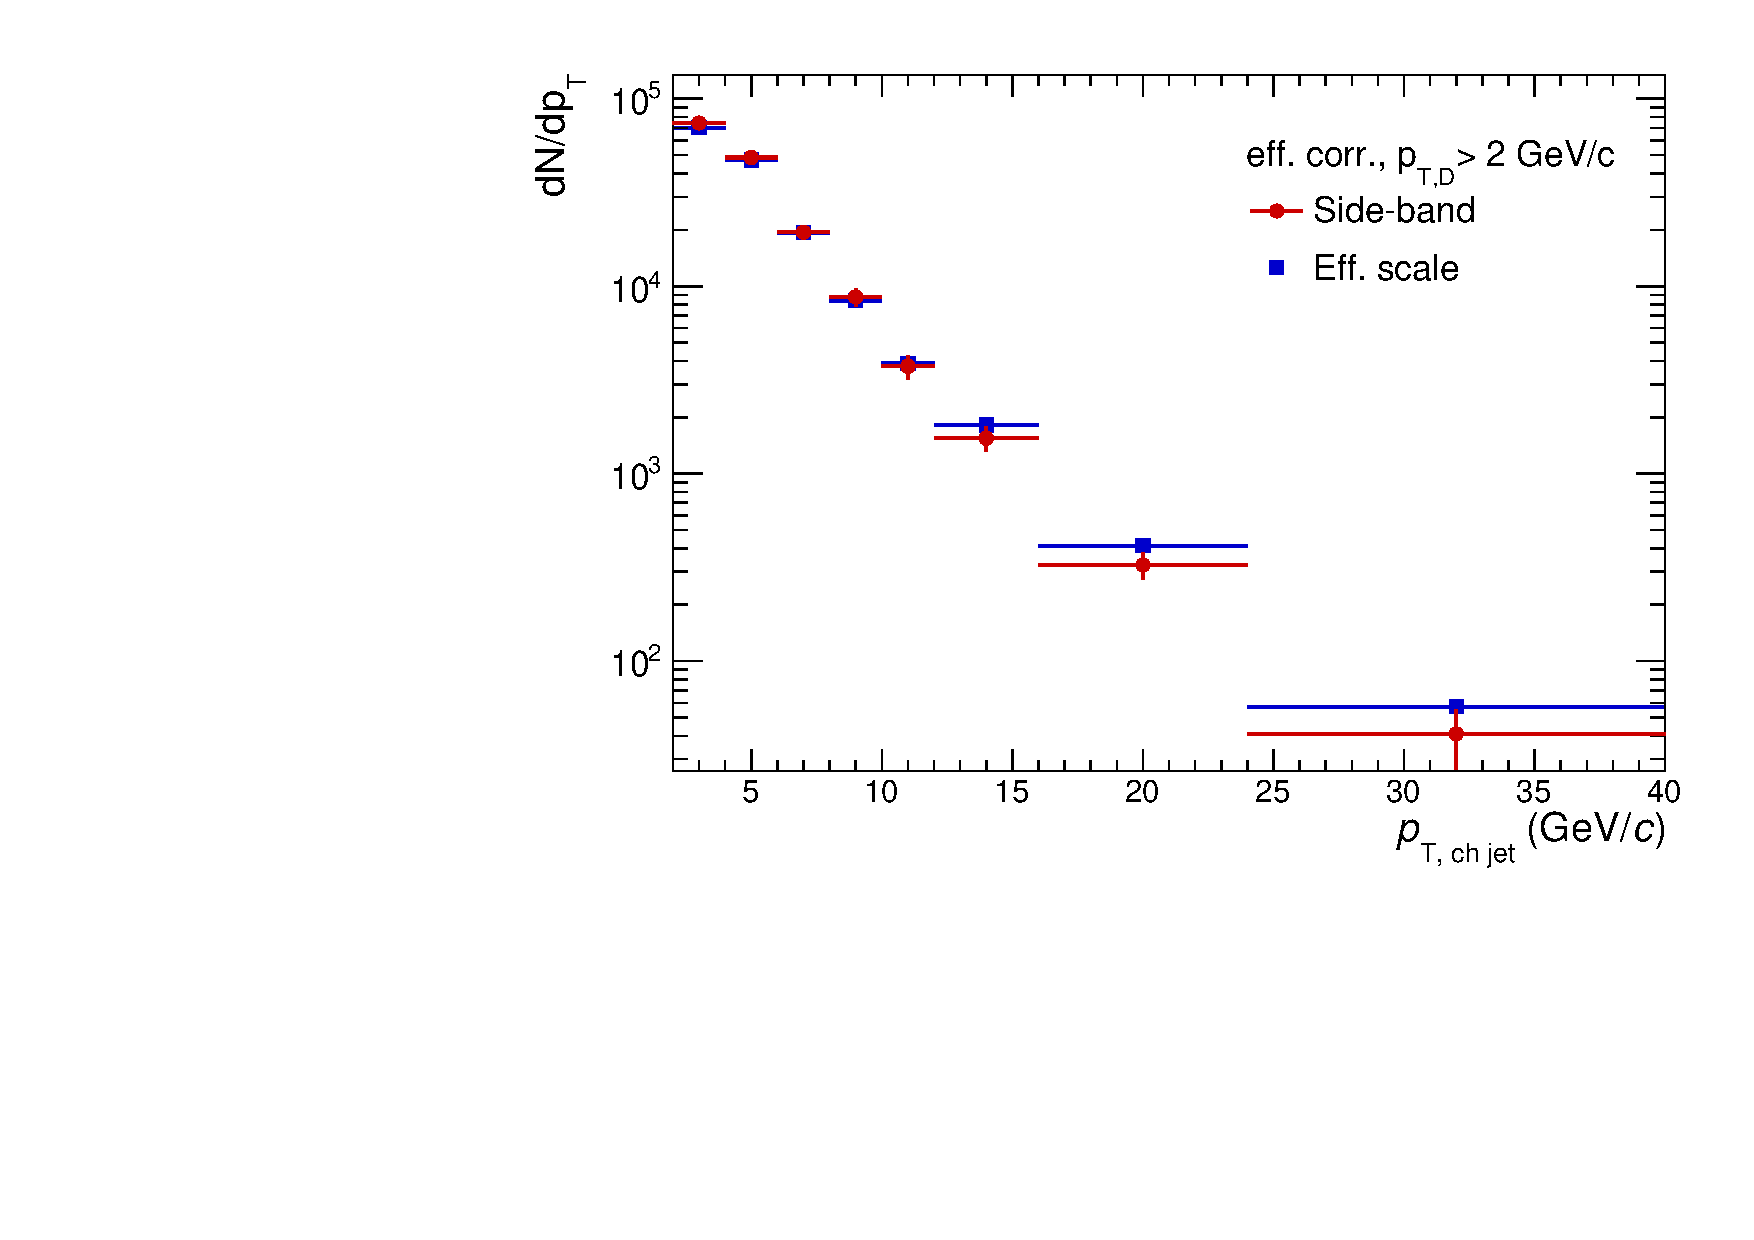
\includegraphics[width=\textwidth]{pPbplots/methodsComparison/DjetSpectra_methodComparison_FASTwoSDD_eff_ptD2}
\caption{Yields}
\end{subfigure}
\begin{subfigure}[b]{0.45\textwidth}
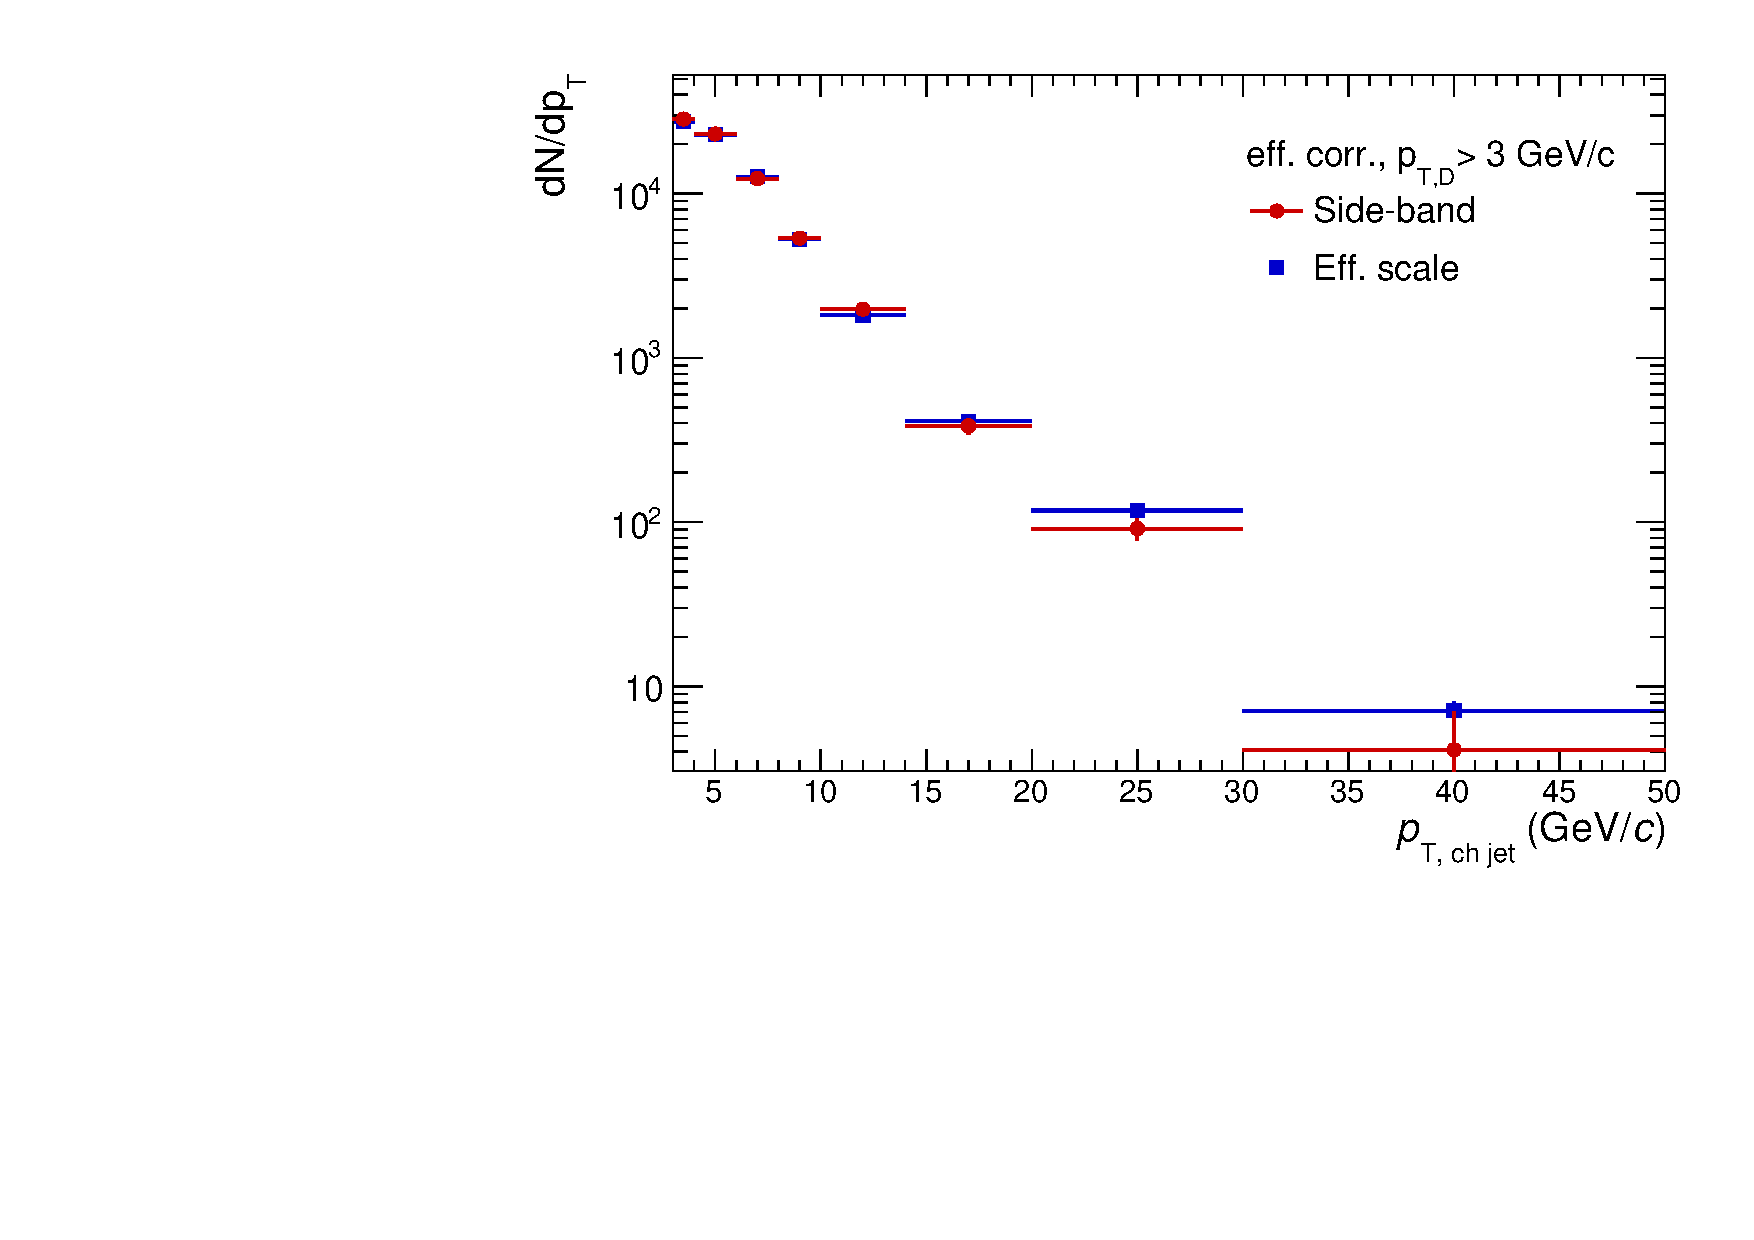
\includegraphics[width=\textwidth]{pPbplots/methodsComparison/DjetSpectra_methodComparison_FASTwoSDD_eff_ptD3}
\caption{Yields}
\end{subfigure}
\begin{subfigure}[b]{0.45\textwidth}
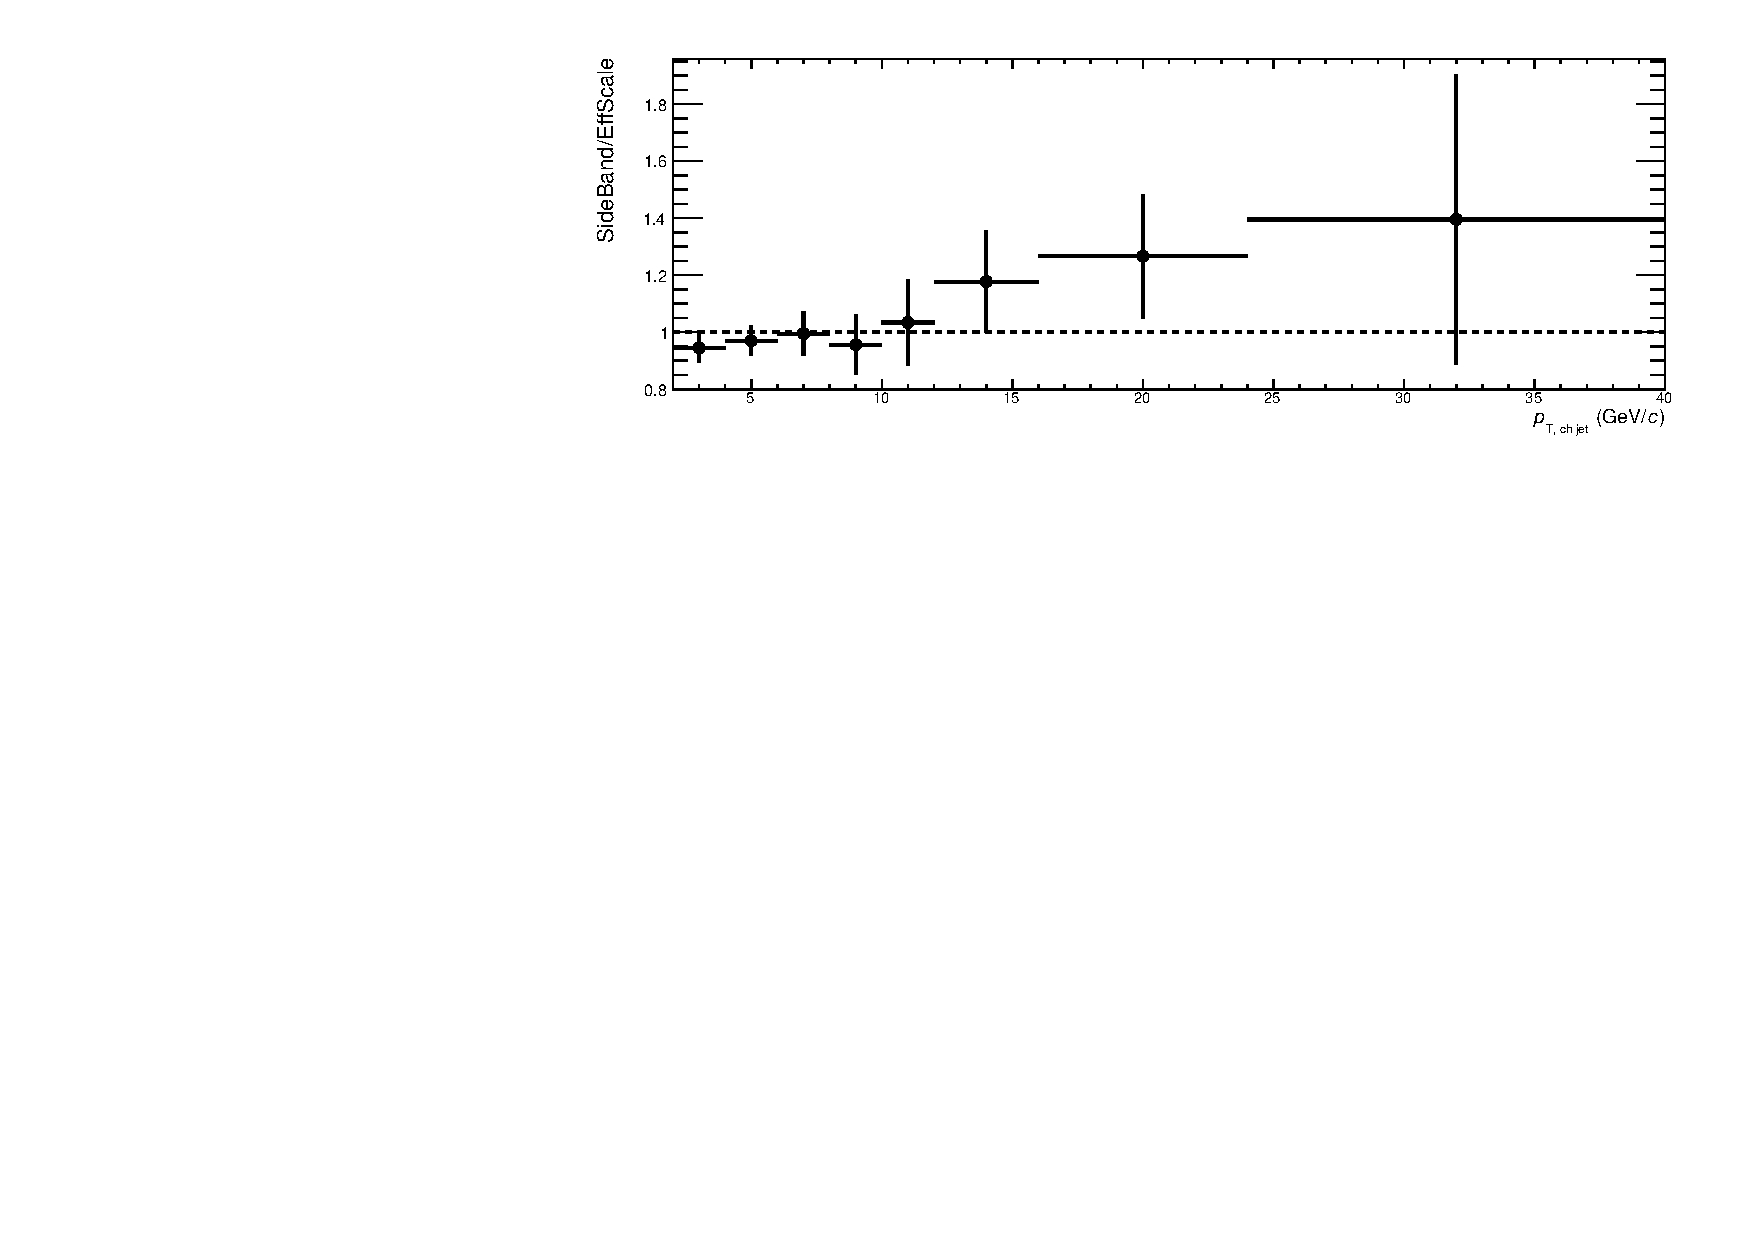
\includegraphics[width=\textwidth]{pPbplots/methodsComparison/DjetSpectraRatio_FASTwoSDD_eff_ptD2}
\caption{Ratio}
\end{subfigure}
\begin{subfigure}[b]{0.45\textwidth}
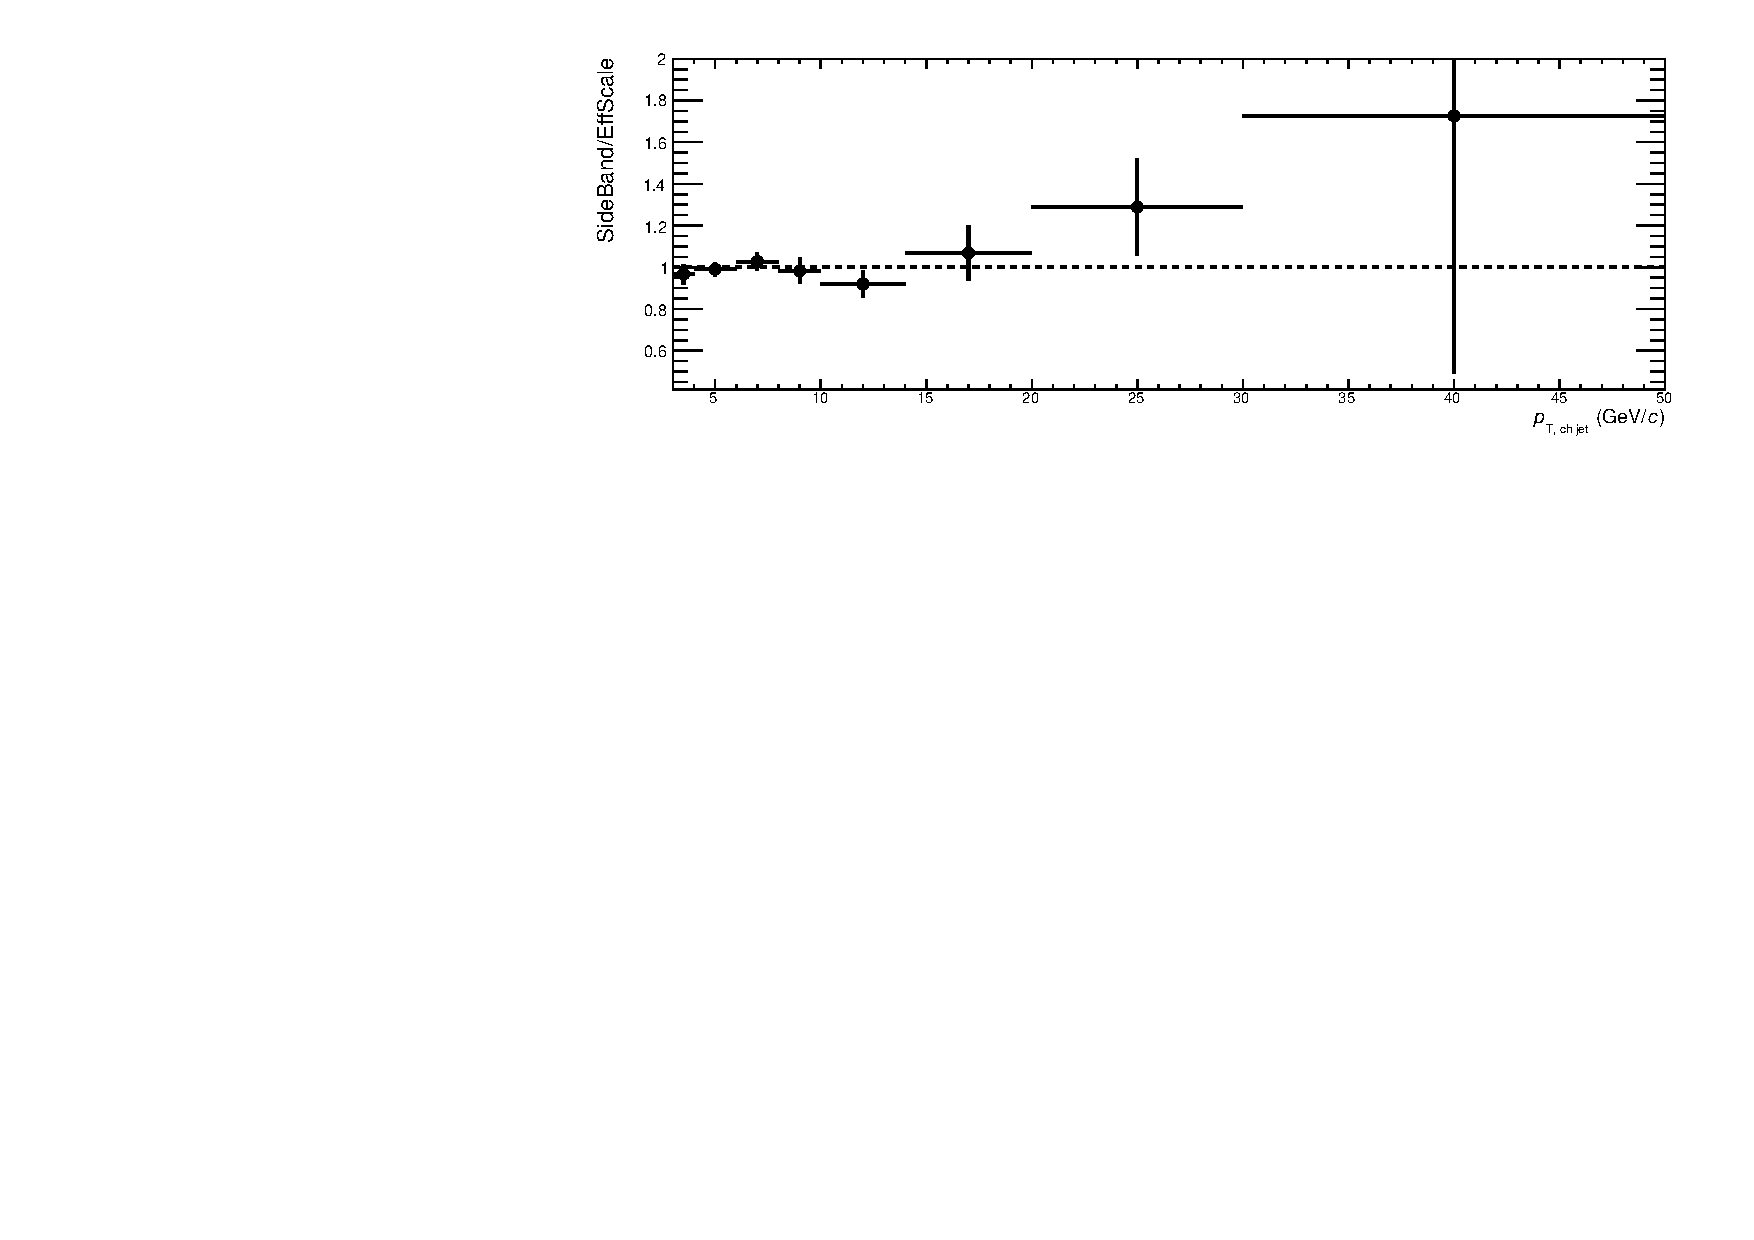
\includegraphics[width=\textwidth]{pPbplots/methodsComparison/DjetSpectraRatio_FASTwoSDD_eff_ptD3}
\caption{Ratio}
\end{subfigure}
\caption{Comparison of the yields obtained using the invariant mass fit method and the side band method for \Dstar-jets in \pPb\ at $\snn=5.02$~TeV, with two cuts on \ptd: $\ptd>2$~\GeVc\ and $\ptd>3$~\GeVc.
Reconstruction efficiency correction is applied in both cases.}
\label{fig:JetPt_pPb_corrDrec}
\end{figure}

\begin{figure}[bth]
\centering
%\begin{subfigure}[b]{0.45\textwidth}
%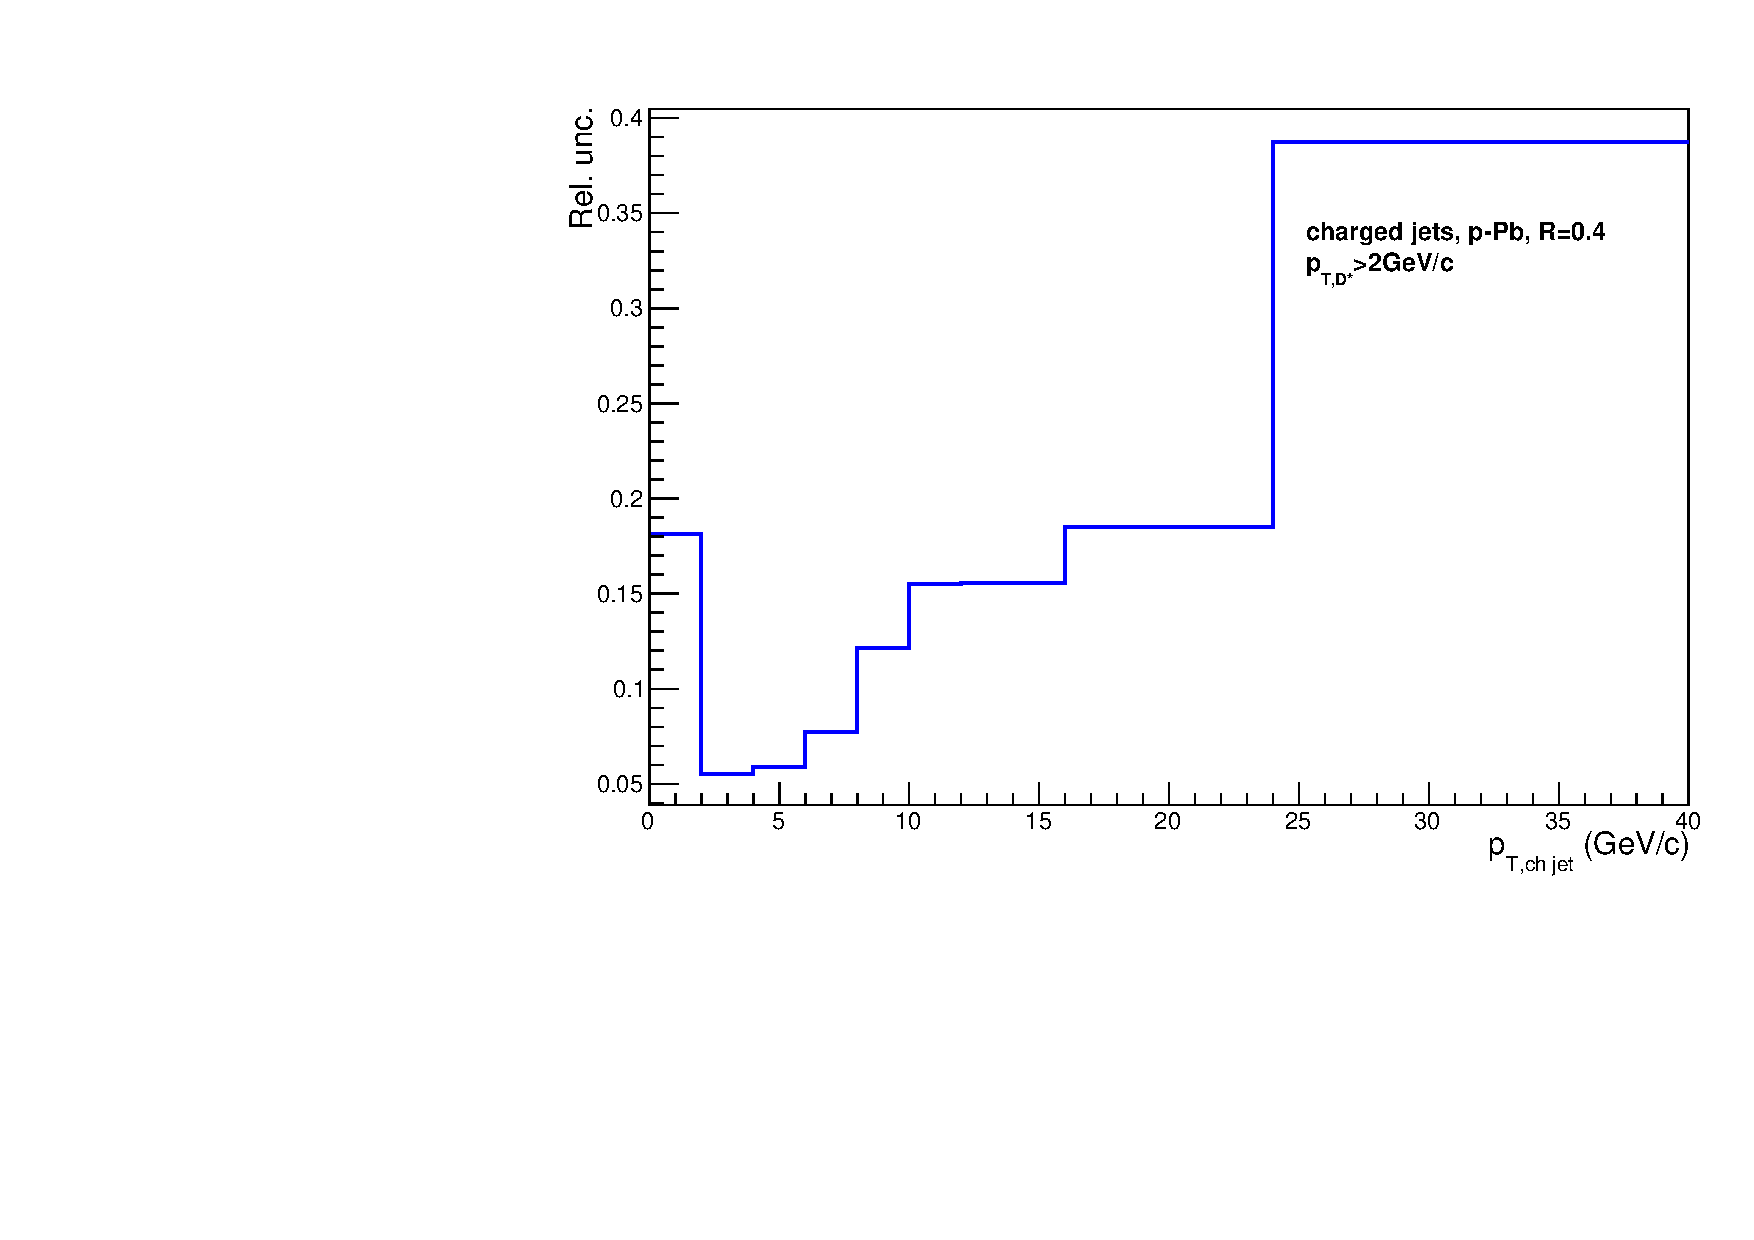
\includegraphics[width=\textwidth]{pPbplots/plotsSB_pt2_noDetails/jetPtSpectrumUnc_SB_Rebin_FASTwoSDD}
%\end{subfigure}
%\begin{subfigure}[b]{0.45\textwidth}
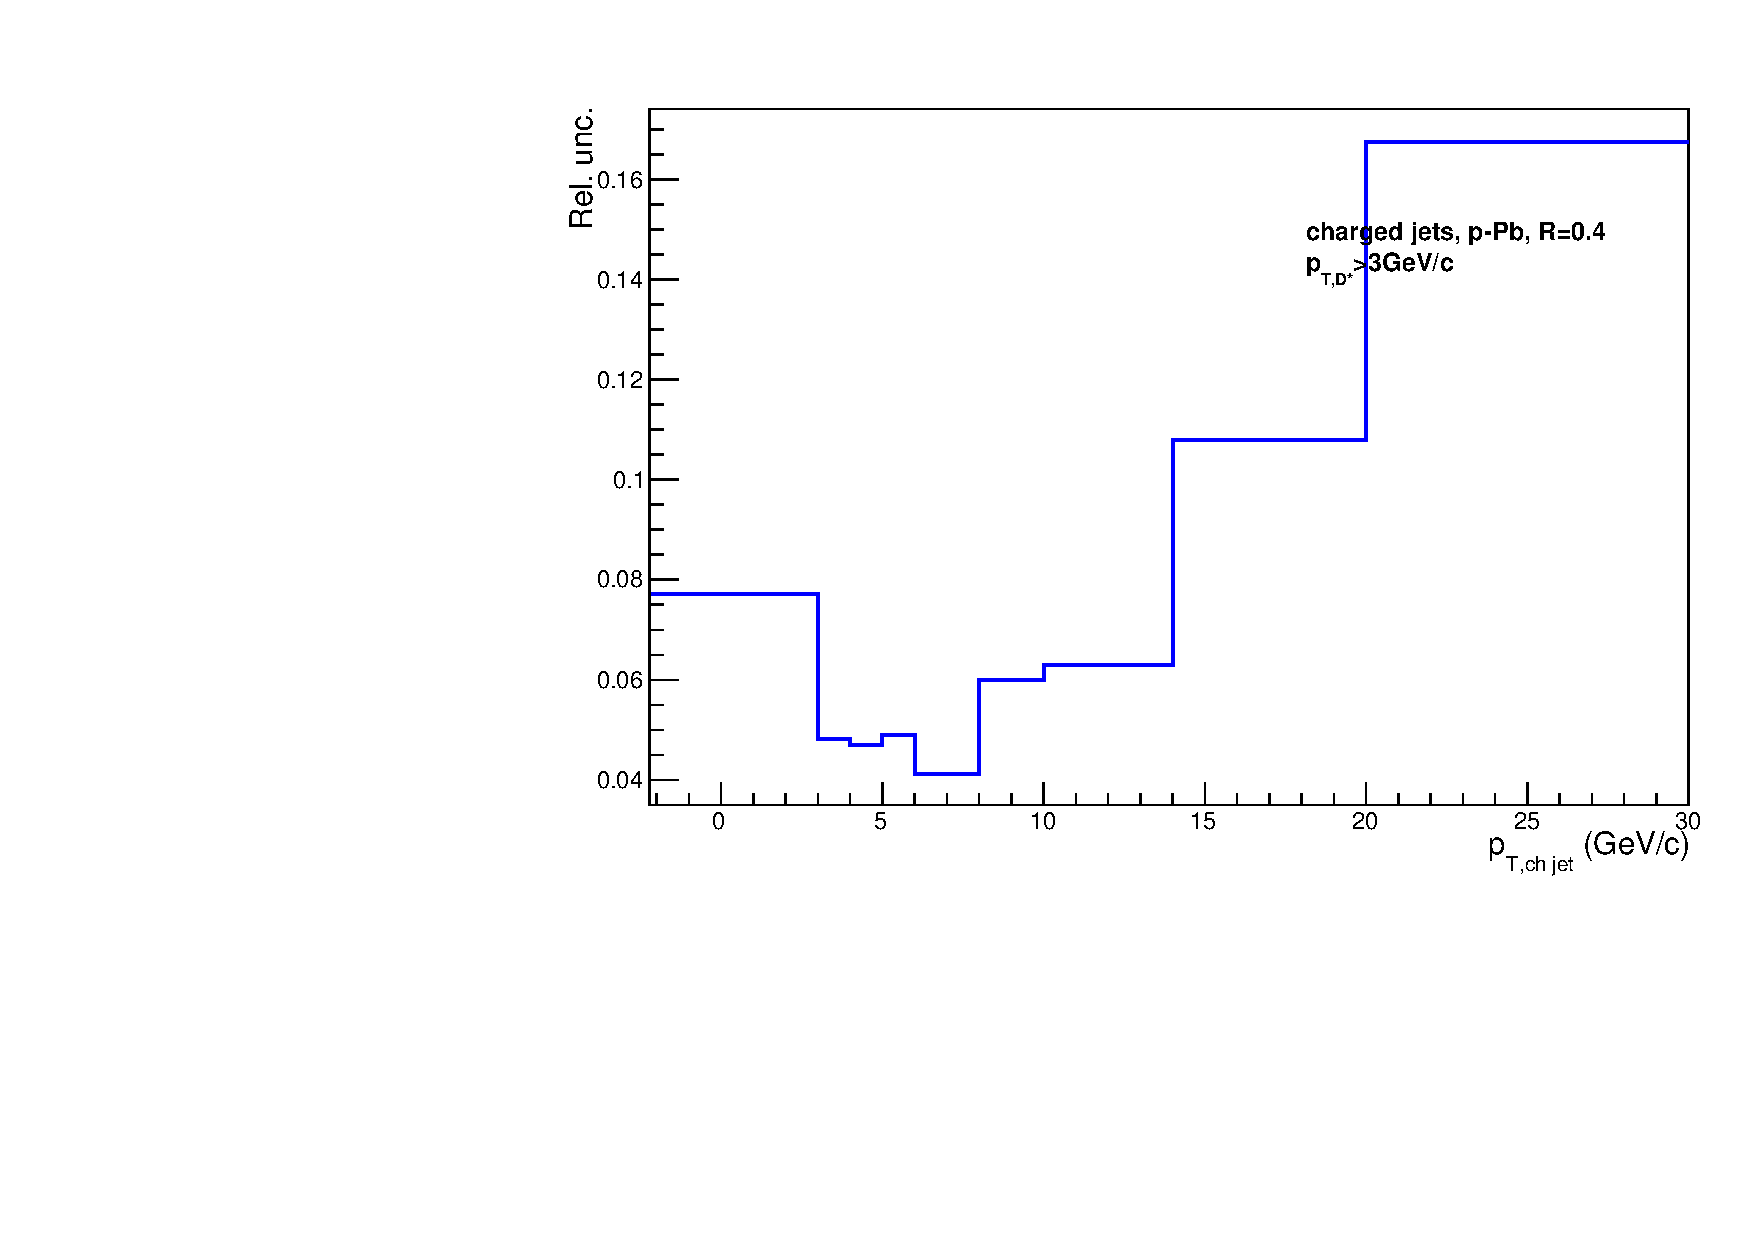
\includegraphics[width=0.45\textwidth]{pPbplots/plotsSB_pt3_noDetails/jetPtSpectrumUnc_SB_Rebin_FASTwoSDD_pTD3}

%\end{subfigure}
\caption{Statistical uncertainties obtained using the side band method for \Dstar-jets in \pPb\ at $\snn=5.02$~TeV, with $\ptd>3$~\GeVc\. Reconstruction efficiency correction is applied.}
\label{fig:JetPt_pPb_SBUnc}
\end{figure}

The default method used for the further analysis is the Side Band method with $\ptd>3$~\GeVc\ cut. The method is more stable, Gaussian fits perform better when they are done in \ptd\ bins, and it is easier to perform the jet spectra analysis with more fine binning if needed.

%%%%%%%%%%%%%%%%%%%%%%%%%%%%%%%%%%%%%%%%%%%%%%%%%%%%%%%%%%%%%%%%%%%%%%
%%%%%%%%%%%%%%%%%%%%%%%%%%%%%%%%%%%%%%%%%%%%%%%%%%%%%%%%%%%%%%%%%%%%%%
%%%%%%%%%%%%%%%%%%%%%%%%%%%%                   UE                     %%%%%%%%%%%%%%%%%%%%%%%%%%%%
%%%%%%%%%%%%%%%%%%%%%%%%%%%%%%%%%%%%%%%%%%%%%%%%%%%%%%%%%%%%%%%%%%%%%%
%%%%%%%%%%%%%%%%%%%%%%%%%%%%%%%%%%%%%%%%%%%%%%%%%%%%%%%%%%%%%%%%%%%%%%

\section{Underlying Event (\pPb\ analysis)}
\subsection{Average Background Momentum Density}
\label{sBackSub}

The Underlying Event (UE) affects the reconstructed jet momentum and need to be subtracted.
The average background density $\rho$ is calculated on an event-by-event basis:

\begin{equation}
\label{eq_rho_pPB}
\rho_{\rm p-Pb} = {\rm median}\left\{\frac{p_{\rm T,jet}^{\kt}}{A_{\rm jet}^{\kt}}\right\} C.
\end{equation}
where $p_{\rm T,jet}^{\kt}$ and $A_{\rm jet}^{\kt}$ are respectively the area and the transverse momentum of
the jets found using the \kt\ algorithm. 
The jet area is estimated by \texttt{FASTJET} using the active ghost method, with a ghost area of $0.005$.
The two leading jets in the event are excluded in order to remove the hard scattering jets from the background.
This approach has been used extensively in jet reconstruction analyses~\cite{ALICE:2014a, ALICE:2015a}.
The corrected jet transverse momentum \ptchjetcorr\ is obtained by subtracting the average background density times the jet area:
\begin{equation}
\label{eq_jet_backsub}
\ptchjetcorr = \ptchjetraw - \rho A_{\rm jet}.
\end{equation}
For \pPb\ collisions a procedure that takes into account sparse environment with the factor $C$, which is the occupancy correction factor, defined as:
\begin{equation}
\label{eq_Cfac}
C = \frac{\sum_{j}A_{j}}{A_{\rm acc}}.
\end{equation}
$A_{j}$ is the area of each \kt\ jet with at least one real track (i.e. excluding ghosts), $A_{\rm acc}$ is the area of charged-particle acceptance.

Figure~\ref{fig:rho} presents $\rho$ distributions calculated in events that include D-jet candidates (the analysed events), and requiring that an event is with the leading jet that has $p_{T}>$ 5 GeV/$c$, for 0-10\% (left) and 20-40\% (right) centrality. The distributions are compared to $\rho$ from events where a presence of D meson within a jet is not required (called inclusive-jet events).

\begin{figure}[bth]
\centering
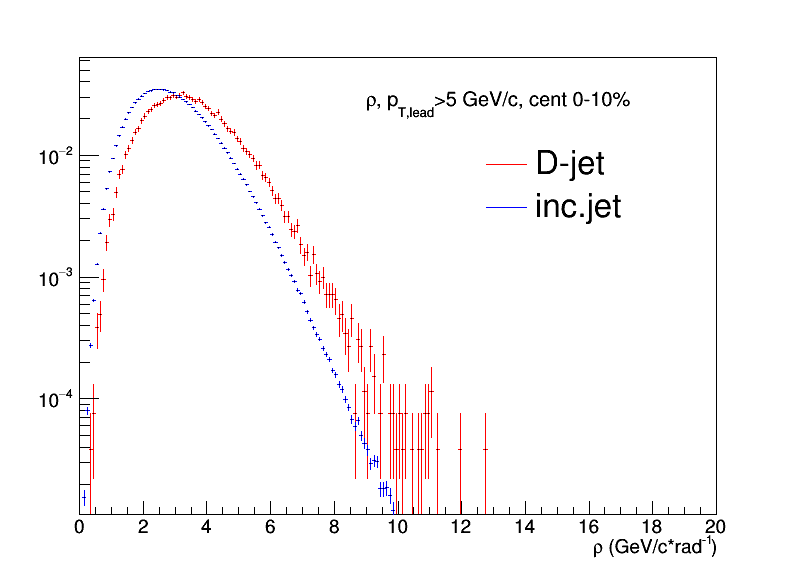
\includegraphics[width=0.45\textwidth]{pPbplots/ResponseMatrix/hRho_ptleadbin5_cent0_10}
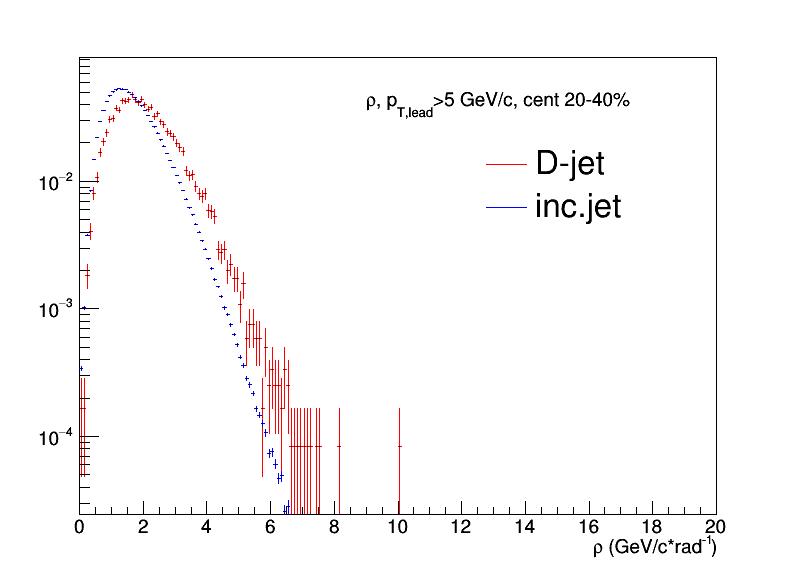
\includegraphics[width=0.45\textwidth]{pPbplots/ResponseMatrix/hRho_ptleadbin5_cent20_40}
\caption{$\rho$ distributions from events with D-jet candidates, and with a leading jet that has $p_{T}>$ 5 GeV/$c$, for 0-10\% (left) and 20-40\% (right) centrality, compared to $\rho$ from events from inclusive-jet events. \pPb\ events with $R=0.4$.}
\label{fig:rho}
\end{figure}

\subsection{Jet Background Fluctuations}
\label{sBackFluc}
The amount of the jet background fluctuation was evaluated using the Random Cone method.
This method consists in generating a random direction in $\eta-\phi$ inside the jet detector acceptance and 
take all tracks in the event that satisfy $\Delta R<R_{\rm cone}$ with $R_{\rm cone}$ equal to the resolution parameter used in the analysis. 
The raw cone \pt\ is the sum of the transverse momenta of all particles within the cone.
The background fluctuation \deltapt\ is calculated as shown in Eq.~\ref{edeltapt}, using events that include D-jet candidates excluding the leading jet in an event, and with the leading jet $p_{T}>$ 5 GeV/$c$. The distribution is shown in Fig.~\ref{fig:DeltaPt} as the left panel. Based on this distribution, a background fluctuation matrix is build which is then used to unfold the measured \Dstar-jet\ \pt spectrum, together with the detector response matrix. The background fluctuation matrix is shown on the right panel of Fig.~\ref{fig:DeltaPt}.

\begin{equation}
\deltapt = p_{\rm T, cone} - \rho \pi R_{\rm cone}^{2}
\label{edeltapt}
\end{equation}

\begin{figure}[bth]
\centering
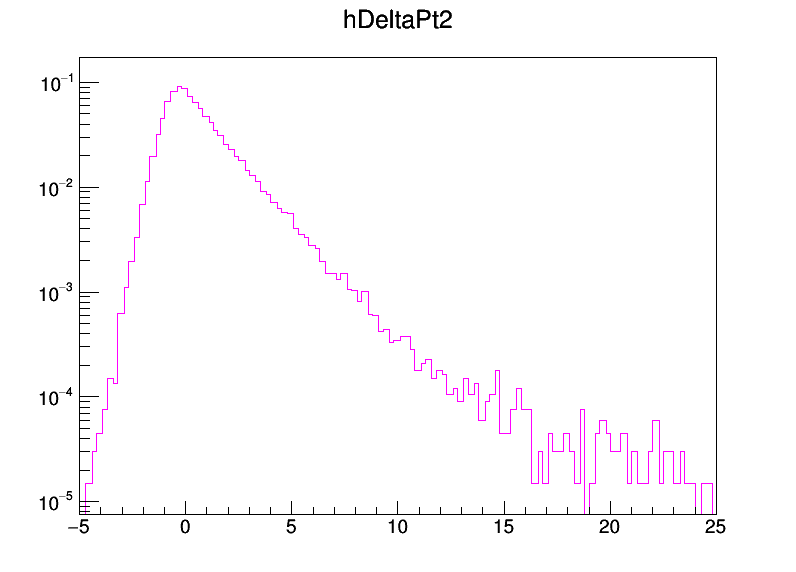
\includegraphics[width=0.45\textwidth]{pPbplots/ResponseMatrix/DeltaPt_Djet5Excl}
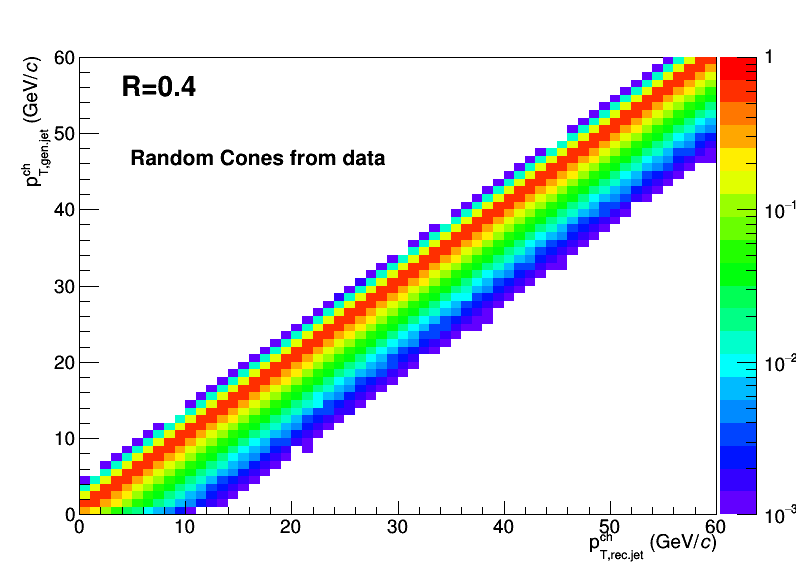
\includegraphics[width=0.45\textwidth]{pPbplots/ResponseMatrix/BkgMatrix_Djet5Excl}
\caption{Left: \deltapt\ distribution obtained with Random Cone method. Right: The background fluctuation matrix built based of the \deltapt\ distribution. \pPb\ events with $R=0.4$.}
\label{fig:DeltaPt}
\end{figure}

%%%%%%%%%%%%%%%%%%%%%%%%%%%%%%%%%%%%%%%%%%%%%%%%%%%%%%%%%%%%%%%%%%%%%%
%%%%%%%%%%%%%%%%%%%%%%%%%%%%%%%%%%%%%%%%%%%%%%%%%%%%%%%%%%%%%%%%%%%%%%
%%%%%%%%%%%%%%%%%%%%%%%%%%%%  DETECTOR RESPONSE  %%%%%%%%%%%%%%%%%%%%%%%%%%%%
%%%%%%%%%%%%%%%%%%%%%%%%%%%%%%%%%%%%%%%%%%%%%%%%%%%%%%%%%%%%%%%%%%%%%%
%%%%%%%%%%%%%%%%%%%%%%%%%%%%%%%%%%%%%%%%%%%%%%%%%%%%%%%%%%%%%%%%%%%%%%

\section{Jet Momentum Detector Response}

The detector response is studied with a Monte Carlo simulation in which particles generated by an event generator are
run through a transport code (GEANT3), that simulates the response of the detector elements, and then the same event reconstruction used in data is performed. Only \ccbar\ events are used.

Two sets of jets are obtained from the same event. One of them is obtained from the generator-level information and the second from the reconstructed signals after the detector simulation. 
The generated and reconstructed jets are matched by looking for the same D meson at both levels (using its MC label).


\subsection{Detector Response Matrix}
\label{Det_Resp}

The detector response matrix for prompt \Dstar-jets is shown in Fig.~\ref{fig:fRMdet_pPb}.
The Monte Carlo production is with Hijing. However, in order to avoid Hijing imperfection of describing the underlying event, only the Pythia part of the production is used to extract the detector response matrix, and the background fluctuations matrix is obtained from data~\ref{sBackFluc}.

\begin{figure}[bth]
\centering
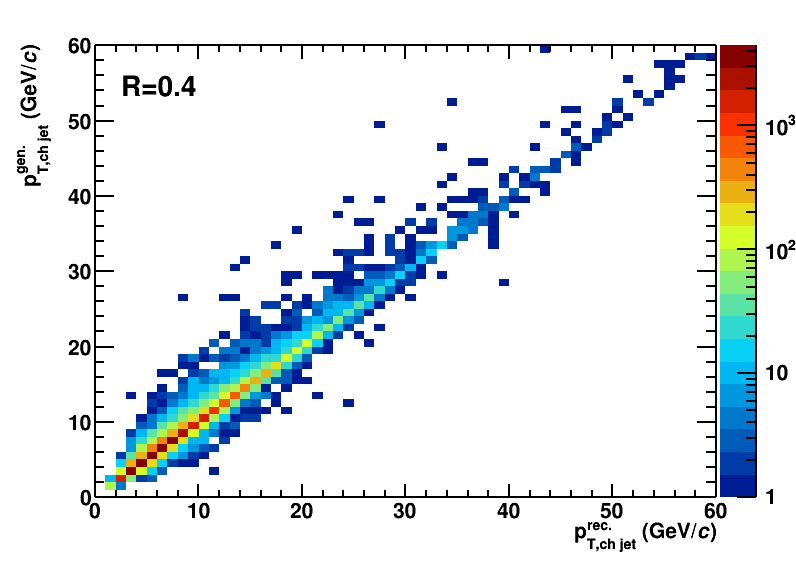
\includegraphics[width=0.49\textwidth]{pPbplots/ResponseMatrix/DetMatrix_Dpt0_100}
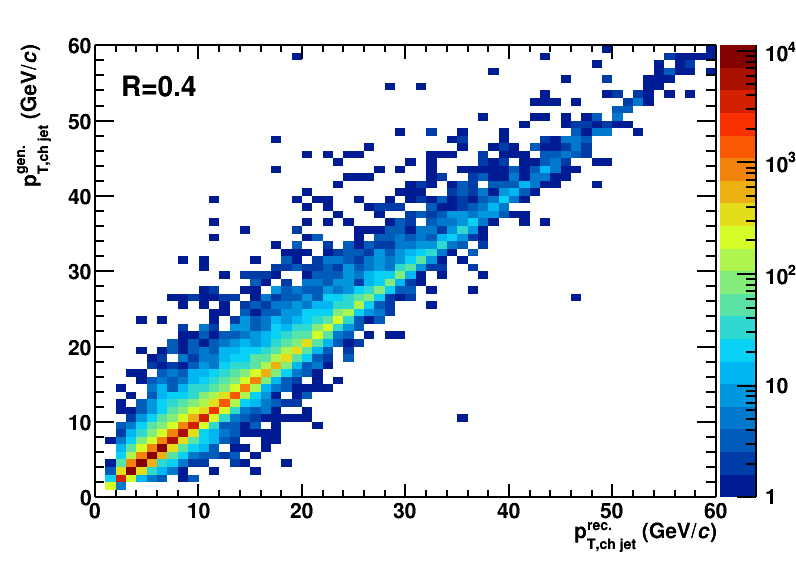
\includegraphics[width=0.49\textwidth]{pPbplots/ResponseMatrix/DetMatrix_Dpt0_100_FD}
\caption{Detector response matrix calculated with the PYTHIA part of the simulation of \pPb\ events at $\snn=5.02$~TeV, for prompt (left) and non-prompt (right) \Dstar-jet.}
\label{fig:fRMdet_pPb}
\end{figure}

The prompt detector response matrix is used to unfold the measured \Dstar-jet \pt spectrum after subtraction of the B feed-down component. The B feed-down is estimated based on simulations, as described later, that is folded with the presented non-prompt detector response matrix combined with the background fluctuation matrix.
%
%Figure~\ref{fig:pPb_ResponseMatrixProj} shows projections of the response on the detector level jet \pt\ in bins of a particle level jet \pt.
%
%\begin{figure}[bth]
%\centering
%\includegraphics[width=0.9\textwidth]{pPbplots/ResponseMatrix/DetMatrixProjectionsComparison_Dpt3_36}
%\caption{Projections of the response on the detector level jet \pt\ in bins of a particle level jet \pt\ calculated with the Pythia simulation of \pPb\ events at $\snn=5.02$~TeV.}
%\label{fig:pPb_ResponseMatrixProj}
%\end{figure}
%
%\subsection{Jet Momentum Resolution}
%
%The jet momentum resolution and energy scale shift are estimated calculating the variable:
%\begin{equation}
%(p_{\mathrm{T,ch\, jet}}^{\mathrm{det}} - p_{\mathrm{T,ch\, jet}}^{\mathrm{part}}) / p_{\mathrm{T,ch\, jet}}^{\mathrm{part}}
%\label{eq:detResp}
%\end{equation}
%for each matched pair of a particle-level jet with a detector-level jet.
%Figure~\ref{fig:pPb_DetectorResponse} shows the probability density distribution of Eq.~\ref{eq:detResp} for \Dstar-jets in \pPb\ collisions at $\snn=5.02$~TeV.
%
%\begin{figure}[bth]
%\centering
%\includegraphics[width=0.9\textwidth]{pPbplots/ResponseMatrix/DetMatrixResProjectionsComparison}
%\caption{Jet momentum resolution calculated with a full simulation of \pPb\ events at $\snn=5.02$~TeV.}
%\label{fig:pPb_DetectorResponse}
%\end{figure}
%
%Figure~\ref{fig:pPb_ResponseMatrixProj} and~\ref{fig:pPb_DetectorResponse} include also a comparison of responses for prompt (red) and non-prompt (blue) \Dstar-jet\ production. The non-prompt response is used at the B feed-down subtraction level, as described in~\ref{sect:FD}.
%


%%%%%%%%%%%%%%%%%%%%%%%%%%%%%%%%%%%%%%%%%%%%%%%%%%%%%%%%%%%%%%%%%%%%%%
%%%%%%%%%%%%%%%%%%%%%%%%%%%%%%%%%%%%%%%%%%%%%%%%%%%%%%%%%%%%%%%%%%%%%%
%%%%%%%%%%%%%%%%%%%%%%%%%%%%           FEED-DOWN            %%%%%%%%%%%%%%%%%%%%%%%%%%%%
%%%%%%%%%%%%%%%%%%%%%%%%%%%%%%%%%%%%%%%%%%%%%%%%%%%%%%%%%%%%%%%%%%%%%%
%%%%%%%%%%%%%%%%%%%%%%%%%%%%%%%%%%%%%%%%%%%%%%%%%%%%%%%%%%%%%%%%%%%%%%

\section{Feed-Down Correction}
\label{sect:FD}

A fraction of the measured D mesons originates from the decays of B mesons. These D mesons are usually referred to as non-prompt,
to distinguish them from the prompt fraction, i.e. the ones that come directly from the fragmentation of a charm quark or decays of higher excited charm states.
The longer decay length of B mesons combined with the topological cuts applied in the D meson selection causes the reconstruction efficiency 
to be higher for the non-prompt fraction compared to the prompt fraction. This is shown in Fig.~\ref{eq_pPb_DrecEff}.
As a consequence, the admixture of the prompt and non-prompt $D-jets$ is biased in a detector-specific way towards the non-prompt.
In order to make meaningful comparisons with theoretical and other experimental results one needs to either correct the bias or remove completely the non-prompt fraction and report only the prompt fraction. Both approaches require to use theoretical models or Monte Carlo simulations.
In ALICE the second approach has been preferred so far, and for this analysis we decided to follow it.

\subsection{Monte Carlo Simulation}

For the D-meson spectra analysis, ALICE has used FONLL~\cite{Cacciari:1998} calculations to estimate the non-prompt fraction~\cite{ALICE:2012d, ALICE:2014d, ALICE:2016a}.
In this analysis however we need to extract the B feed-down fraction also as a function of the jet kinematics, therefore this approach is not applicable.
We decided to use POWHEG~\cite{Alioli:2010}, a Monte Carlo event generator known to reasonably reproduce FONLL calculations and previous experimental results~\cite{Cacciari:2012b}.
The second part of the parton shower and the fragmentation into hadrons is provided by PYTHIA6 (Perugia-2011 tune). In addition a boost was applied in order to account for an asymmetric \pPb\ collision system. 

We generated 25 M \ccbar\ events and 25 M \bbbar\ events for the baseline parameters: 
$m_{\rm c} = 1.5$~\GeVcsq, $m_{\rm b} = 4.75$~\GeVcsq, $\mu_{\rm R} = \mu_{\rm F} =\mu_{0} = \sqrt{m^2+\pt^2}$,
where $m_{\rm c}$ and $m_{\rm b}$ are receptively the charm and beauty masses, $\mu_{\rm R}$ and $\mu_{\rm F}$ are respectively the renormalization and factorization scale factors.  Used based PDF set is: CT10NLO and nPDF: EPS09NLO.
%Figures~\ref{fig:pp_POWHEGvsFONLL_ccbar} and~\ref{fig:pp_POWHEGvsFONLL_bbbar} show a comparison of the D-meson spectra generated by POWHEG+PYTHIA with a FONLL calculation, for \ccbar\ and \bbbar\ events respectively.

The reconstruction of D-meson jets is performed in the POWHEG+PYTHIA events using the same procedure used for the main data analysis.


\subsection{Feed-Down Subtraction}
The B feed-down (FD) is subtracted from the measured D-meson jet \pt\ spectra by scaling the cross-section of D-meson jets obtained from the analysis of the POWHEG+PYTHIA simulation by the integrated luminosity of the analyzed data, according to Eq.~\ref{eq:bFDsub}:
\begin{equation}
N^{\rm c\rightarrow\Dstar}(\ptchjetdet) = 
N^{\rm c,b\rightarrow\Dstar}(\ptchjetdet) - 
R_{\rm det}^{\rm b\rightarrow\Dstar}(\ptchjetdet,\ptchjetgen) \otimes \sum_{\ptd} \frac{\epsilon^{\rm b\rightarrow\Dstar}(\ptd)}{\epsilon^{\rm c\rightarrow\Dstar}(\ptd)} N^{\rm b\rightarrow\Dstar}_{\rm POWHEG}(\ptd,\ptchjetgen),
\label{eq:bFDsub}
\end{equation}
where:
\begin{itemize}
\item $N^{\rm c\rightarrow\Dstar}(\ptchjetdet)$ is the efficiency-corrected measured yield after FD subtraction; 
\item $N^{\rm c,b\rightarrow\Dstar}(\ptchjetdet)$ is the efficiency-corrected measured yield before FD subtraction;
\item $R_{\rm det}^{\rm b\rightarrow\Dstar}(\ptchjetdet,\ptchjetgen)$ is the detector response matrix of the \pt\ of non-prompt \Dstar-jets;
\item the symbol $\otimes$ is to be interpreted as the standard product of the response matrix times the vector of the yields in bins of \ptchjetgen;
\item $\epsilon^{\rm c\rightarrow\Dstar}(\ptd)$ and $\epsilon^{\rm b\rightarrow\Dstar}(\ptd)$ are respectively the reconstruction efficiencies of prompt and non-prompt \Dstar\ mesons;
\item $N^{\rm b\rightarrow\Dstar}_{\rm POWHEG}(\ptd,\ptchjetgen)$ is the cross-section of \Dstar-jets from the POWHEG simulation scaled by the integrated luminosity of the analyzed data.
\end{itemize}

%\begin{figure}[bth]
%\centering
%\includegraphics[width=.8\textwidth]{pp_plots/BFeedDown/DetectorJetPtResolutionPromptNonPromptComparison}
%\caption{Jet momentum resolution for different ranges of \ptchjetgen\ for prompt (red full markers) and non-prompt (open blue markers) \Dzero-jets.}
%\label{fig:res_prompt_nonprompt}
%\end{figure}

The POWHEG \Dstar-jet spectrum is weighted with the ratio of the prompt over non-prompt efficiency because it is subtracted from the measured yield.

%Projections of prompt and non-prompt \Dstar-jets response matrices in slices \ptchjetgen are shown in Fig.~\ref{fig:pPbres_prompt_nonprompt}. There are small differences between the prompt and non-prompt response seen. 
There are differences between the prompt and non-prompt response, for this reason the FD has to be subtracted before unfolding the measured spectrum; furthermore, as illustrated in Eq.~\ref{eq:bFDsub}, the spectrum obtained
from the POWHEG simulation is smeared using the response of non-prompt \Dstar-jets. Combined response matrix used to fold the simulated non-prompt spectrum is shown in Fig~\ref{fig:pPb_ResponseMatrix_nonprompt}.
Figure~\ref{fig:pPbFD_corr} compares the measured \Dstar-jet \pt\ spectrum with the FD spectrum and the subtracted spectrum.

\begin{figure}[bth]
\centering
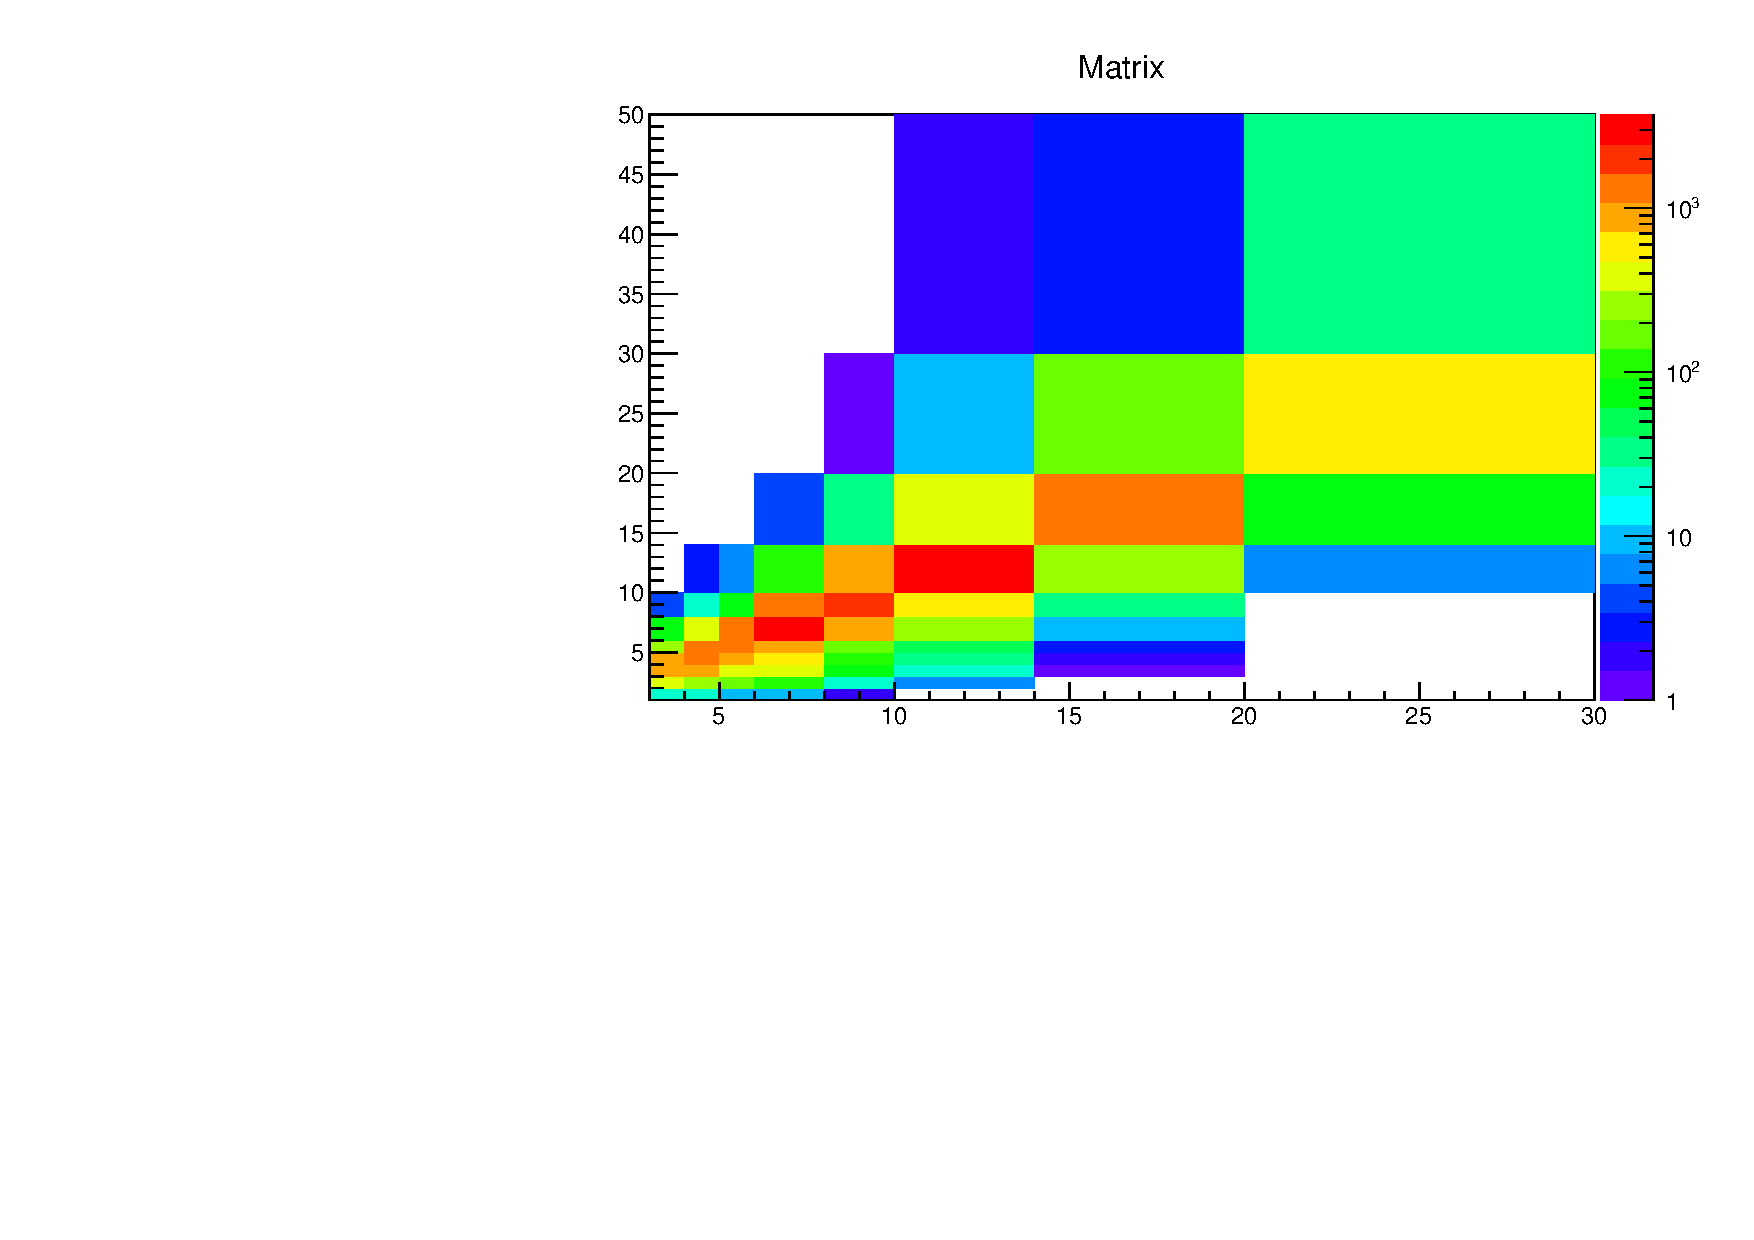
\includegraphics[width=0.6\textwidth]{pPbplots/ResponseMatrix/combMatrixFD_DjetExcl5}
\caption{Combined response matrix calculated with a full simulation of \pPb\ events at $\snn=5.02$~TeV.}
\label{fig:pPb_ResponseMatrix_nonprompt}
\end{figure}

\begin{figure}[bth]
\centering
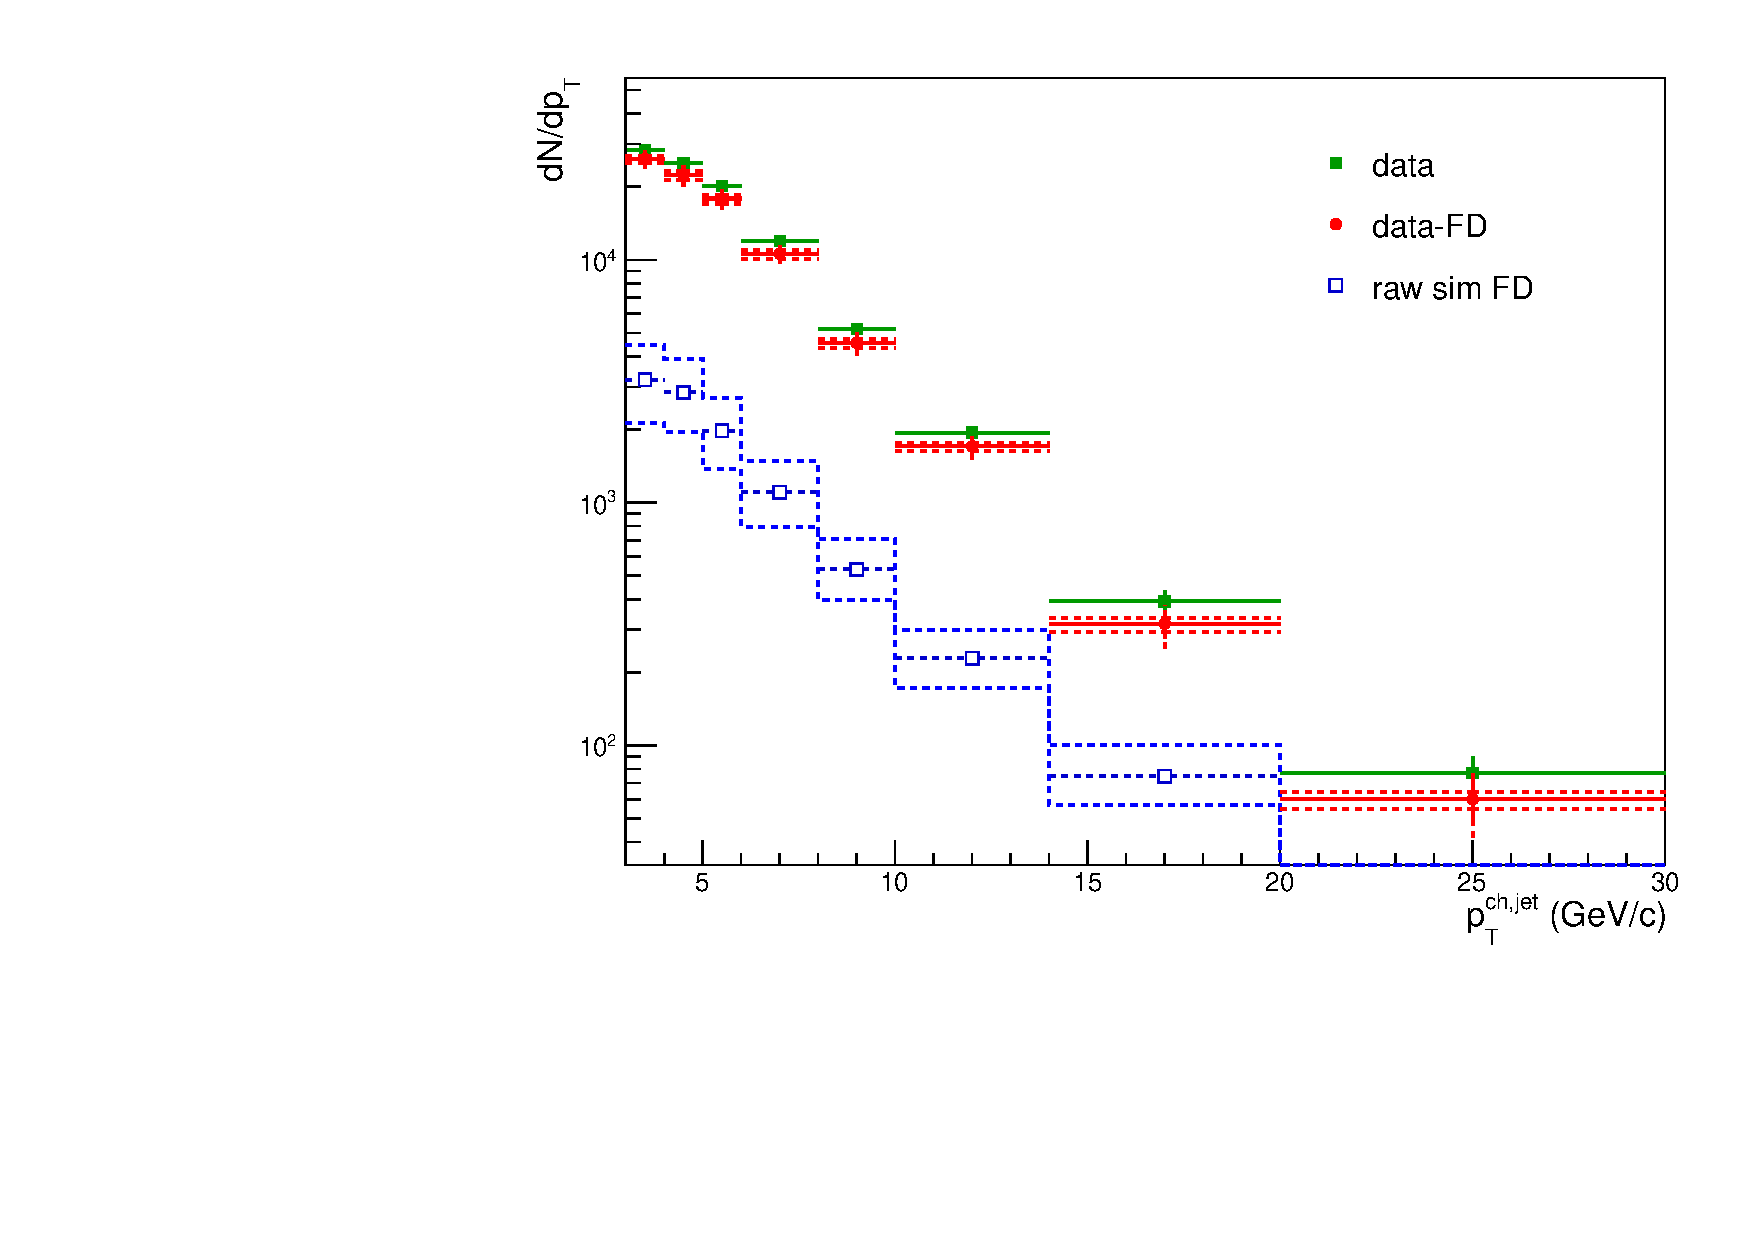
\includegraphics[width=.53\textwidth]{pPbplots/jetSpectra/JetPtSpectra_FDsub}
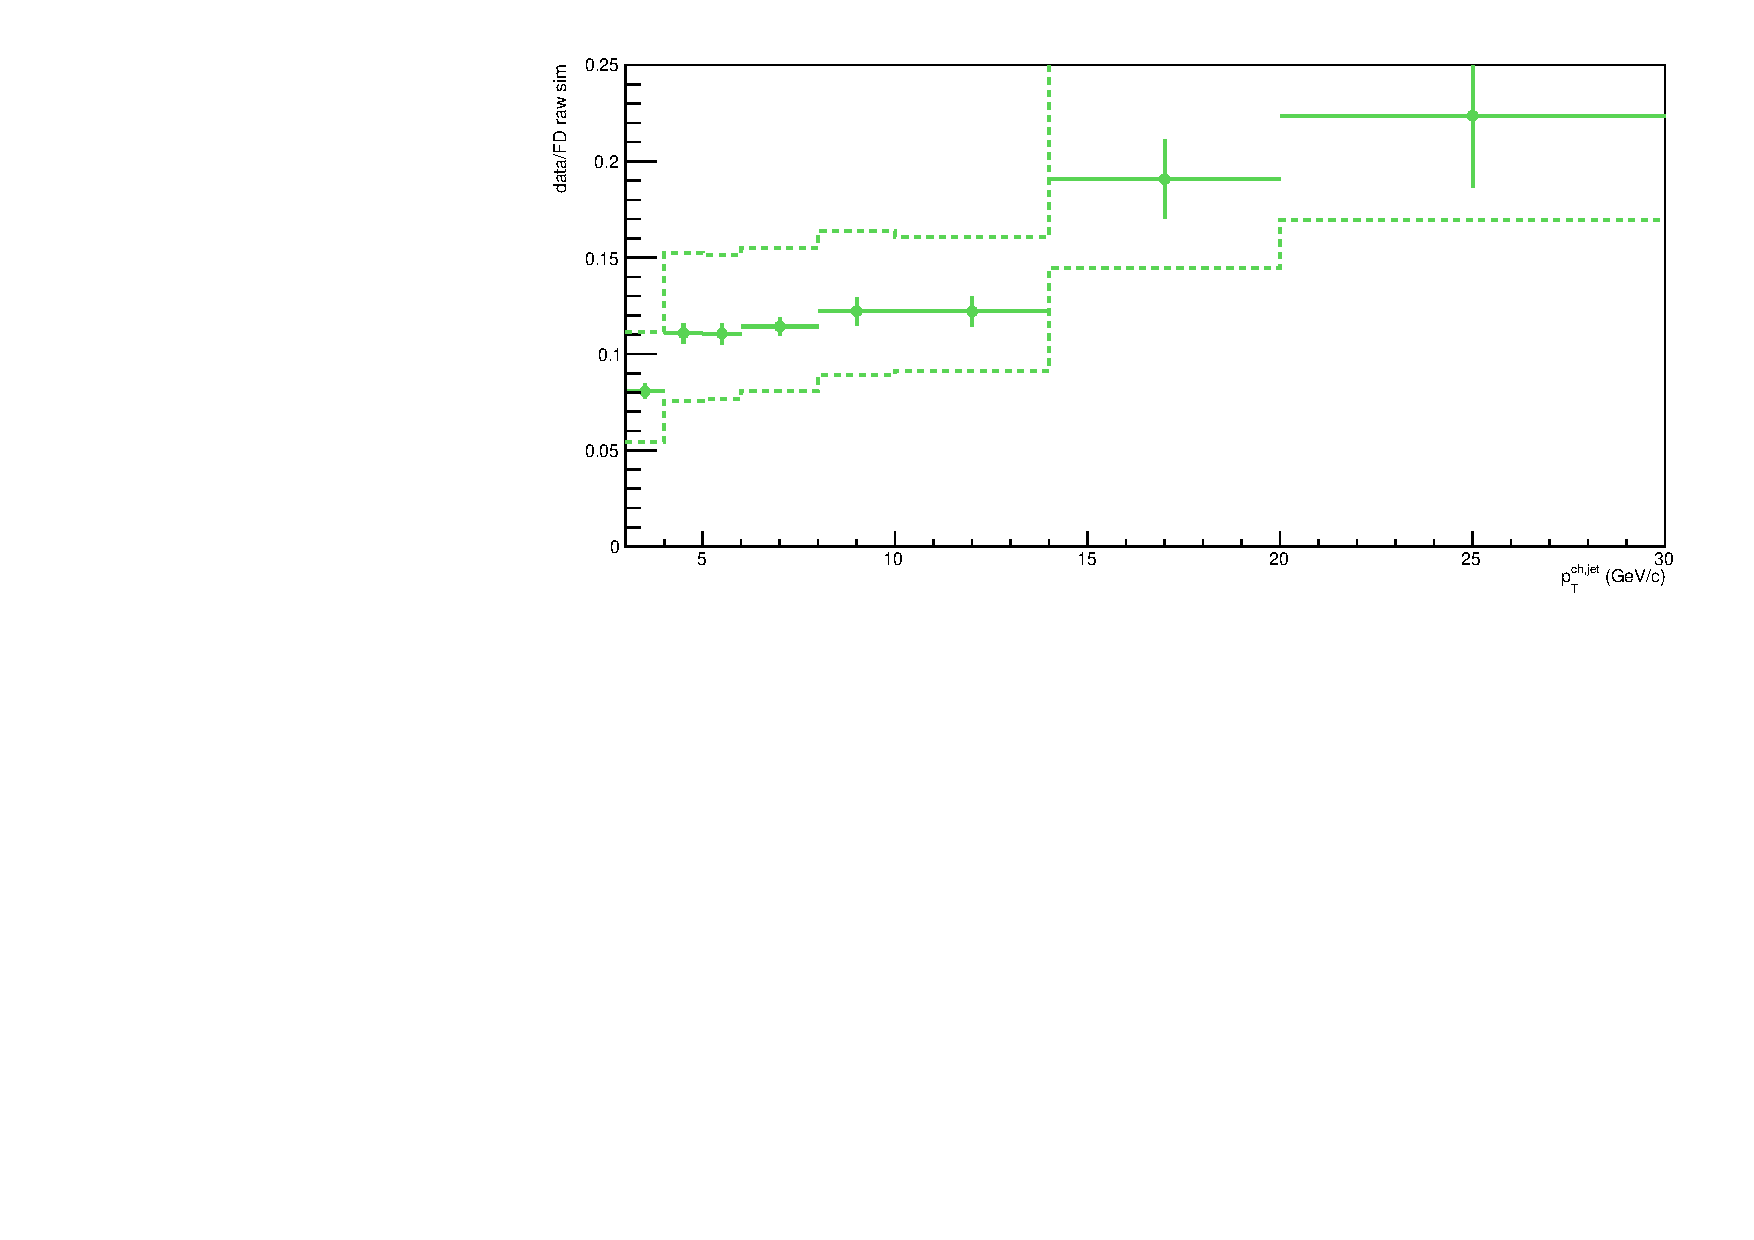
\includegraphics[width=.45\textwidth]{pPbplots/jetSpectra/FDratio}
\caption{Left: Efficiency-corrected measured \Dstar-jet spectrum in \pPb\ collisions at $\snn=5.02$~TeV before FD correction (green) and after FD correction (red). The FD spectrum is also plotted (blue) with its uncertainties. Right plots show ratio of non-prompt to inclusive \Dstar-jet spectrum.}
\label{fig:pPbFD_corr}
\end{figure}


%%%%%%%%%%%%%%%%%%%%%%%%%%%%%%%%%%%%%%%%%%%%%%%%%%%%%%%%%%%%%%%%%%%%%%
%%%%%%%%%%%%%%%%%%%%%%%%%%%%%%%%%%%%%%%%%%%%%%%%%%%%%%%%%%%%%%%%%%%%%%
%%%%%%%%%%%%%%%%%%%%%%%%%%%%           UNFOLDING            %%%%%%%%%%%%%%%%%%%%%%%%%%%%
%%%%%%%%%%%%%%%%%%%%%%%%%%%%%%%%%%%%%%%%%%%%%%%%%%%%%%%%%%%%%%%%%%%%%%
%%%%%%%%%%%%%%%%%%%%%%%%%%%%%%%%%%%%%%%%%%%%%%%%%%%%%%%%%%%%%%%%%%%%%%

\section{Unfolding}
\label{sect:unfResults}
Due to detector finite momentum resolution and tracking inefficiency the jet \pt\ spectra measured as described
in the previous sections are distorted. In addition, in \pPb\ collisions, fluctuations in the background momentum density
introduce additional distortions. These distortions are detector-specific and do not allow a direct comparison
with theoretical models and other independent experimental results.

In order to correct for these distortions, we first need to assess the detector performance and quantify
the detector response to the D-meson jets. In addition, for the \pPb\ analysis the background fluctuations are quantified in a
fully data-driven fashion.

Figure~\ref{pPb_ResponseMatrix} shows a combined response matrix in \pPb\, used for the jet \pt\ spectra unfolding.
The matrix is rebinned according to the binning used for the final jet \pt\ spectra. Then, the unfolding matrix, a distribution used as a prior and the corrected jet \pt\ spectrum obtained from the data are passed to the unfolding algorithm. The algorithm returns an unfolded jet \pt spectrum. As a prior, the spectrum obtained from the Monte Carlo simulation at the generator level is used.

\begin{figure}[bth]
\centering
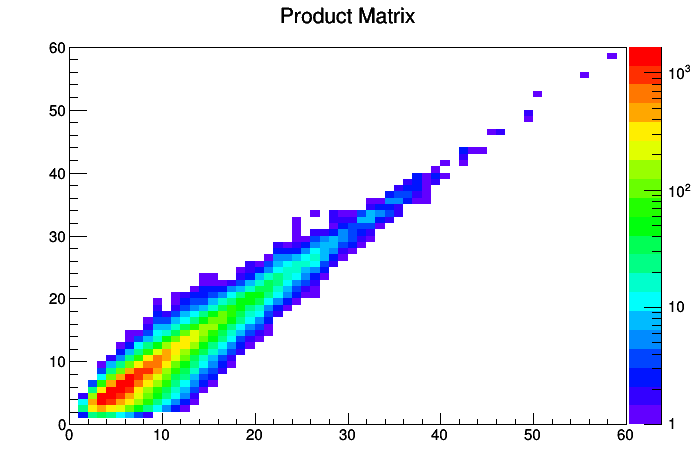
\includegraphics[width=0.49\textwidth]{pPbplots/ResponseMatrix/PythiaRM__Djet5Excl_2_bayes5_weight_MatrixProd}
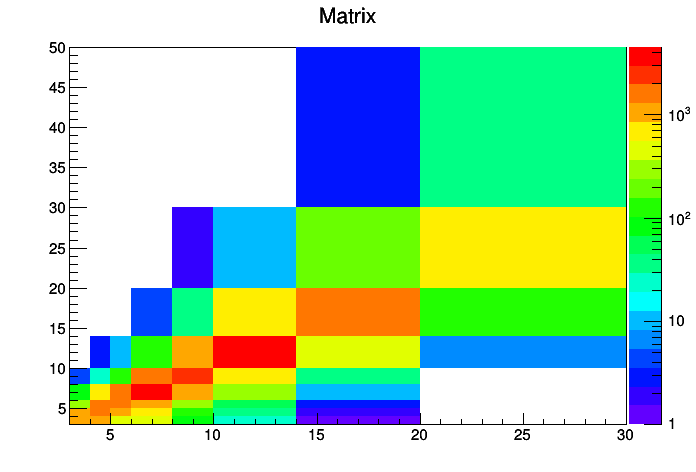
\includegraphics[width=0.49\textwidth]{pPbplots/ResponseMatrix/PythiaRM__Djet5Excl_2_bayes5_weight_Matrix}
\caption{Combined response matrix calculated with a full simulation of \pPb\ events at $\snn=5.02$~TeV.}
\label{fig:pPb_ResponseMatrix}
\end{figure}

\begin{figure}[bth]
\centering
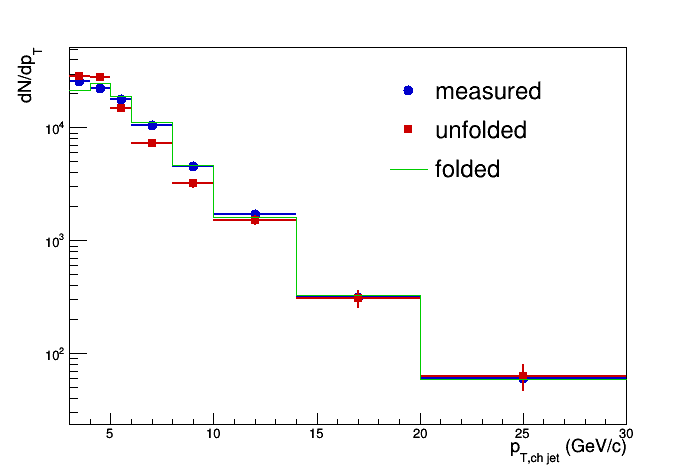
\includegraphics[width=0.55\textwidth]{pPbplots/ResponseMatrix/PythiaRM__Djet5Excl_2_bayes5_weight_UnfSpectrum}
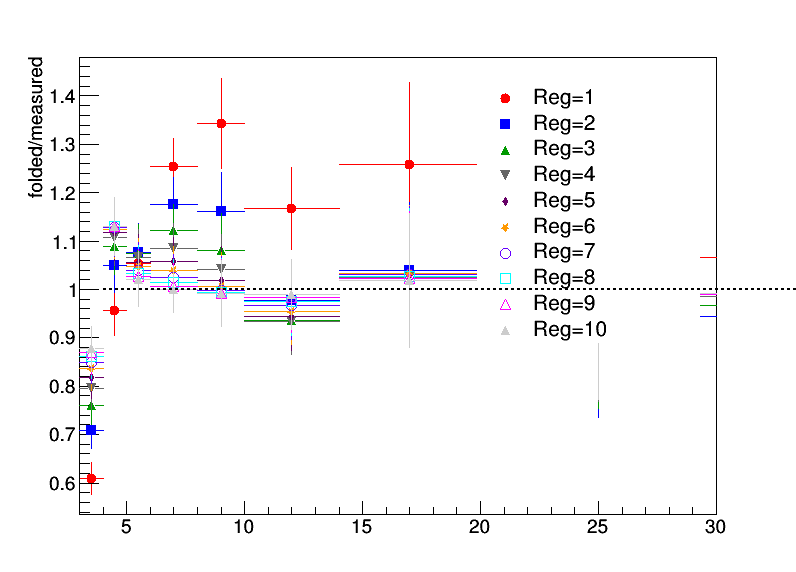
\includegraphics[width=0.44\textwidth]{pPbplots/ResponseMatrix/PythiaRM__Djet5Excl_2_bayes5_weight_foldedRatio}
\caption{Left: Corrected jet \pt spectrum before (blue) and after (red) the unfolding procedure (Bayesian method with five iterations), \pPb\ events at $\snn=5.02$~TeV. Right: ratio to the measured spectrum to the folded for up to 10 iterations in the Bayesian unfolding, the considered jet \pt\ range is above 5 GeV/$c$.}
\label{fUnfSpec_pPb}
\end{figure}

Figure~\ref{fUnfSpec_pPb} presents corrected for the reconstruction efficiency and B feed-down jet \pt\ spectra before the unfolding (blue) and after the unfolding (red), for the side-band method.
Unfolding is done with Bayesian and SVD (see~\ref{sUnfoldSys}) techniques using the \texttt{RooUnfold} software package. The default method is the Bayesian with five iterations. The green line represents folded back spectrum, and is compared to the measured jet spectrum before unfolding with different iterations in the Bayes unfolding - right panel of Fig.~\ref{fUnfSpec_pPb}, a considered in the analysis jet \pt\ range is above 5 GeV/$c$.

Comparison of unfolded spectra with different methods and priors is presented in the systematic uncertainties section. 

\section{Systematic Uncertainties}

We considered the following sources of systematic uncertainties:

\begin{easylist}[itemize]
& Raw yield extraction
& D-Meson Selection Cuts
& B Feed-Down
& Unfolding and background fluctuation matrix
& Tracking Efficiency
& \pt\ Shape of the Monte Carlo Spectrum
\end{easylist}

\subsection{Raw Yield Extraction}
The stability and systematics of the raw yield extraction has been assessed using the \texttt{MultiTrial} framework developed by the D2H group.
This framework performs the fit of the invariant mass distribution many times varying several conditions, such us binning, fixed vs. free parameters,
background function, fit range.

The following variations were included in the assessment of the systematics for the raw yield extraction of \Dstar\ jets in \pPb:
\begin{itemize}
\item fixed $\sigma=\sigma_{\rm MC}$;
\item fixed $\sigma=1.15\sigma_{\rm MC}$
\item fixed $\sigma=0.85\sigma_{\rm MC}$
\item free $\sigma$ and fixed $m_{0}=m_{\rm PDG}$;
\item fixed $\sigma=\sigma_{\rm MC}$ and $m_{0}=m_{\rm PDG}$;
\item free $\sigma$ and free $m_{0}$;
\item background functions: power-law and power-law $\times$ exponential;
\item lower limit of fit range: $0.140$, $0.142$~\GeVcsq;
\item upper limit of fit range: $0.158$, $0.160$~\GeVcsq;
\item rebin by factor 2
\end{itemize}
Figure~\ref{fig:AverageRawYieldVsDefault_pPB} shows the average of the yields obtained in each of these variations compared with the yields obtained with default fit settings as outlined in Section~\ref{sect:raw_yield}.
The systematic uncertainties are calculated as the root-mean-square of all the yields obtained in the multi-trial fits and are shown in Fig.~\ref{fig:MultiTrialRMS_pPB}.

\begin{figure}[bth]
\begin{center}
\begin{subfigure}[b]{.45\textwidth}
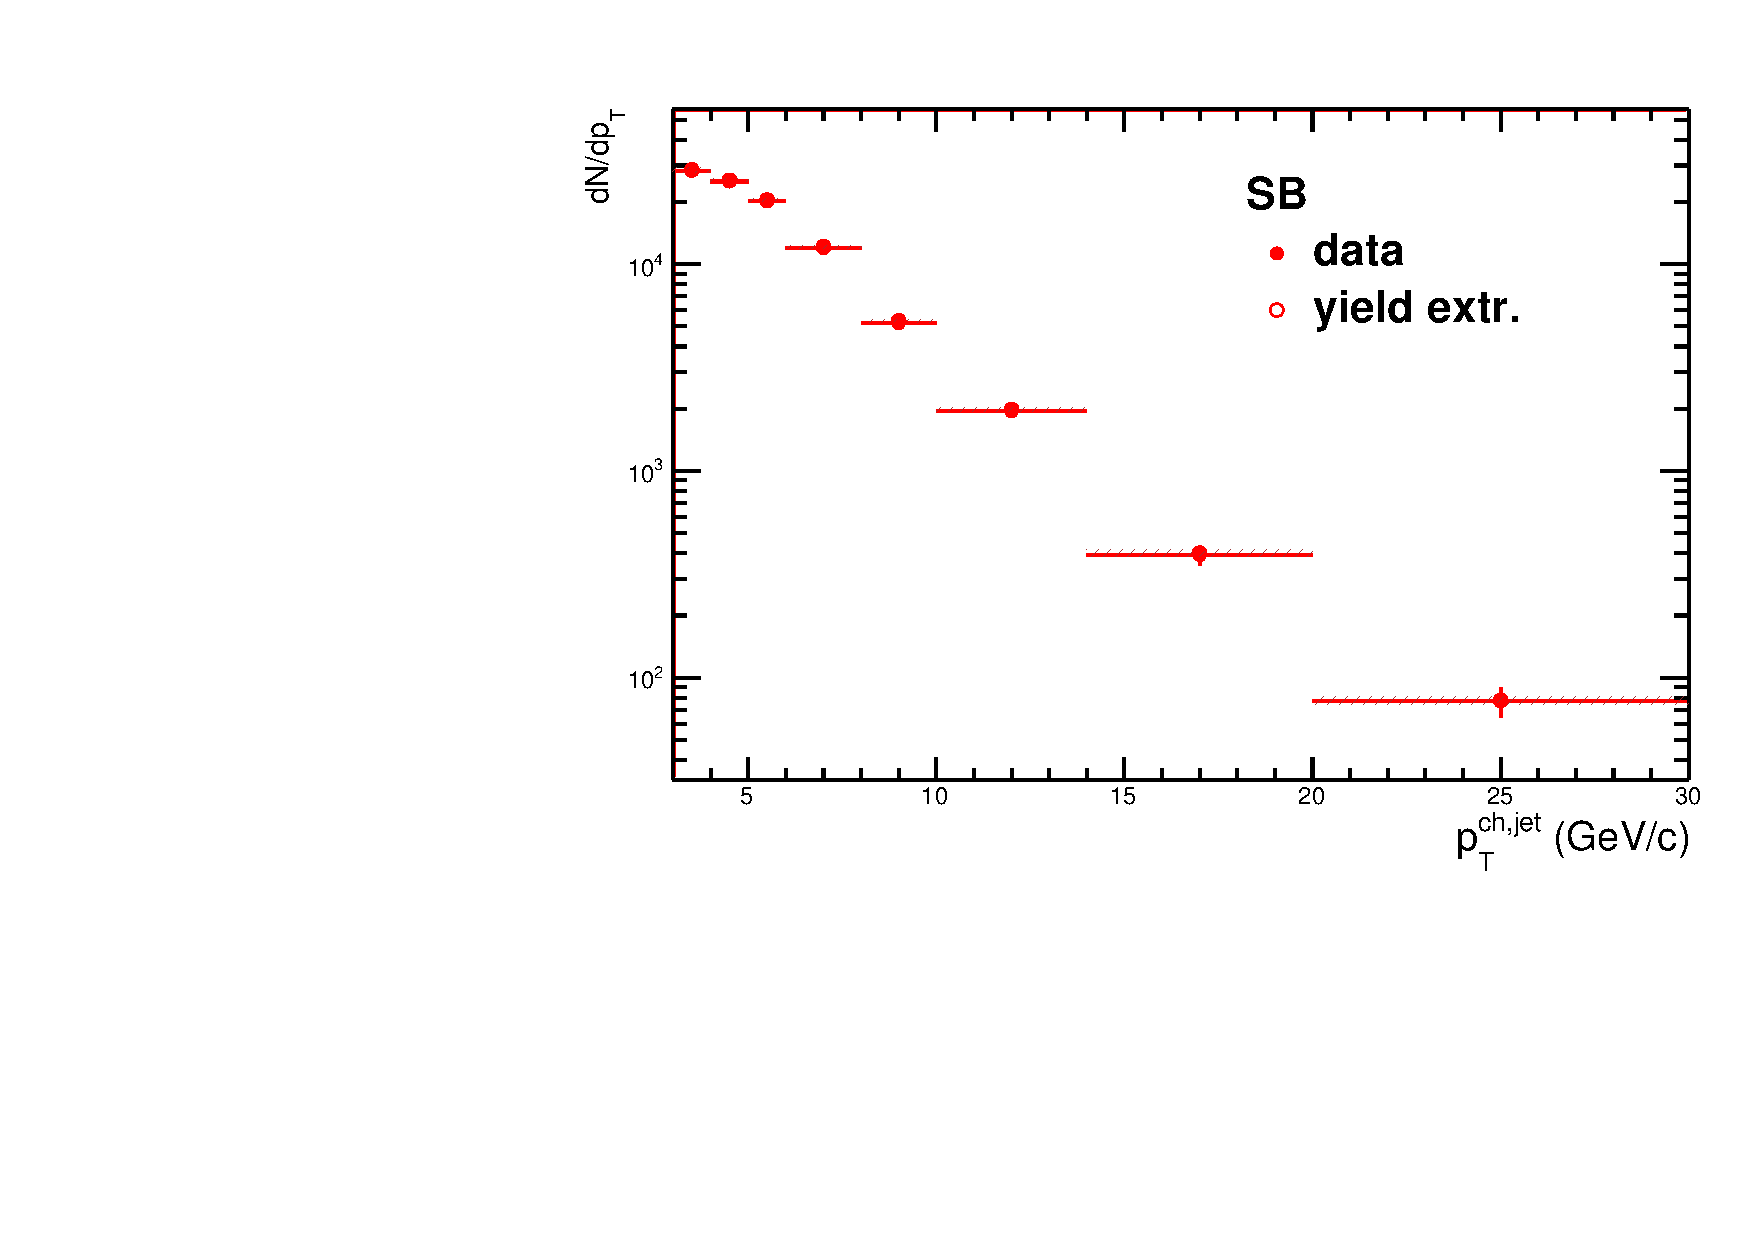
\includegraphics[width=\textwidth]{pPbplots/yieldExtraction/jetPtComparison_DataMVariation_SB}
%\caption{Yields}
\label{fig:AverageRawYieldVsDefault_Yields_pPb}
\end{subfigure}
\begin{subfigure}[b]{.45\textwidth}
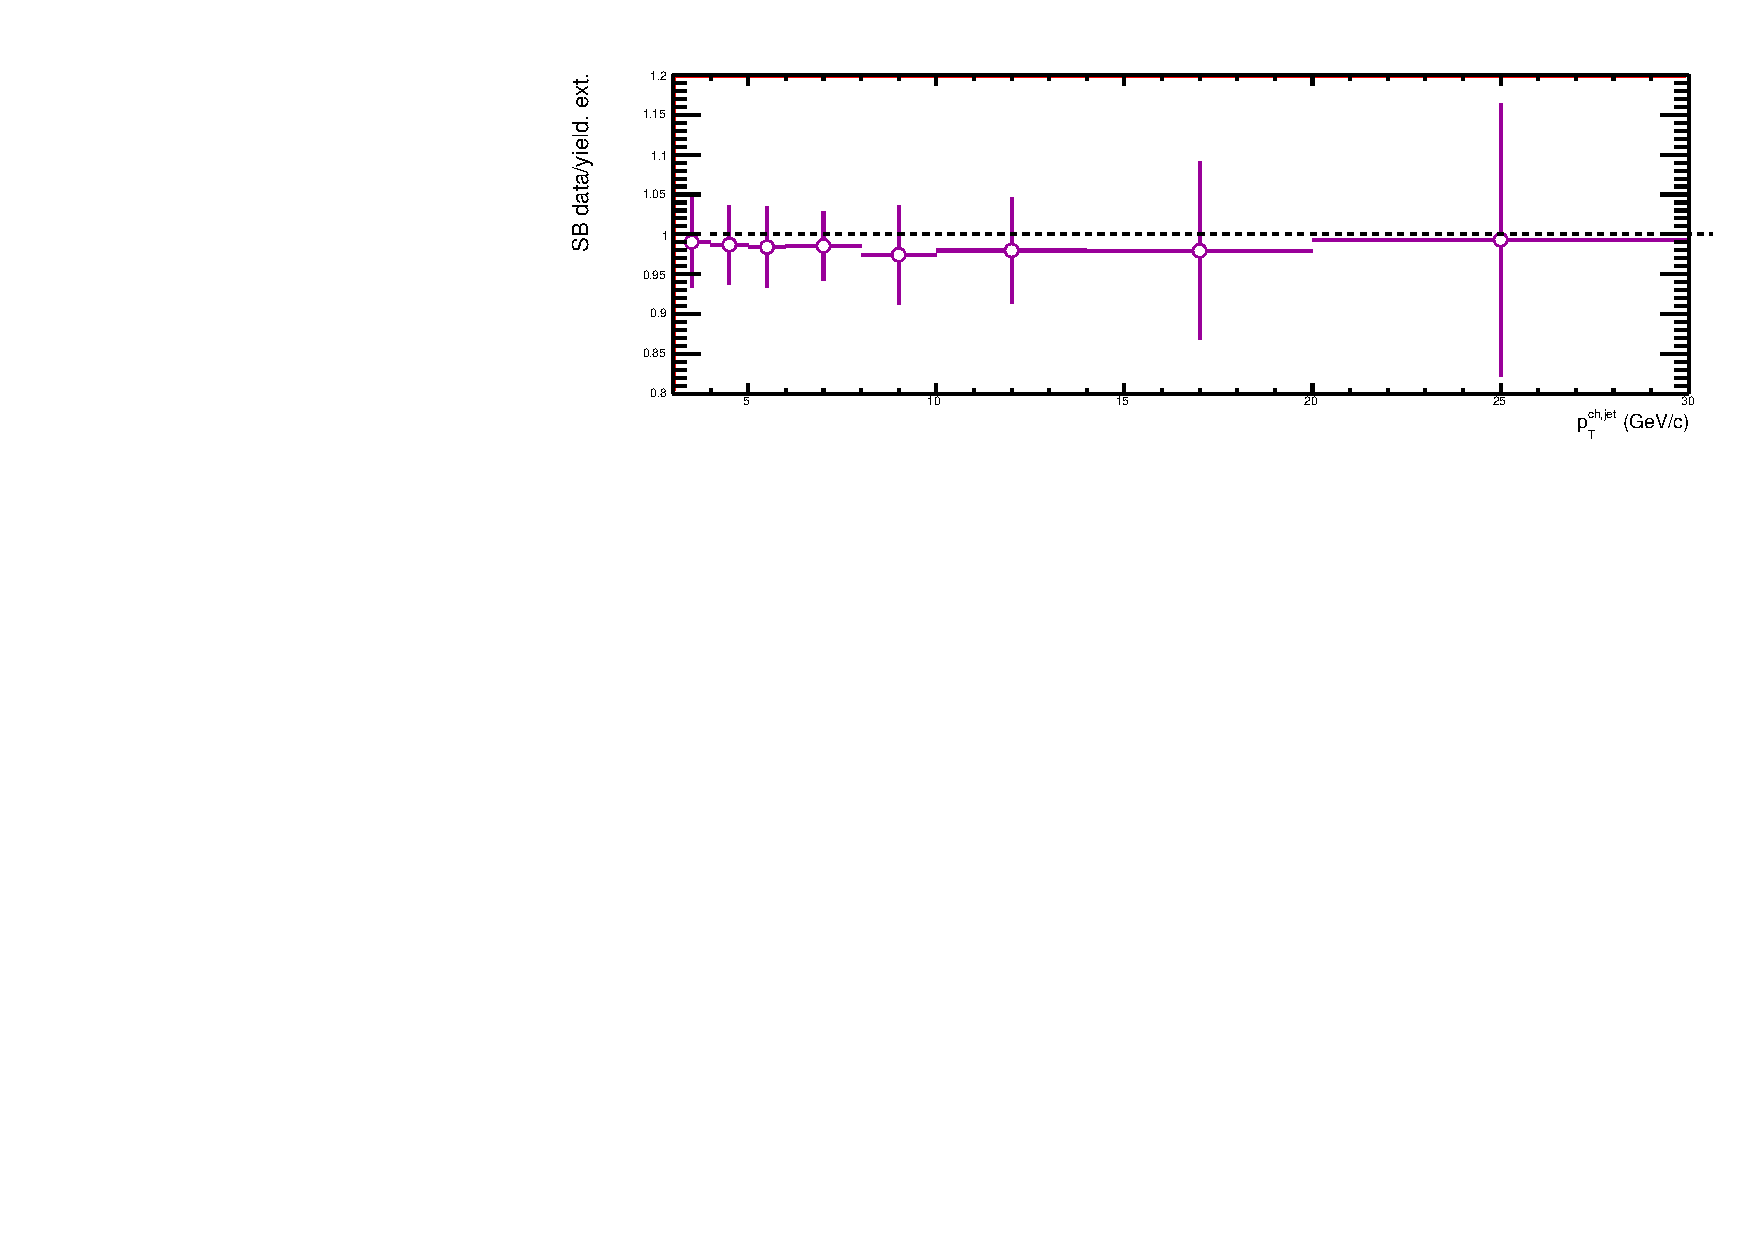
\includegraphics[width=\textwidth]{pPbplots/yieldExtraction/SBRatio}
%\caption{Yield from multi-trial}
\label{fig:MultiTrialSys_pPb}
\end{subfigure}
\caption{\Dstar-jet yields in \pPb\ collisions obtained  with the side-band method.
On the left, the yields are shown with the default fit conditions (full markers) with error bars representing the statistical uncertainty and with the average of
the multi-trial fit with filled rectangles representing the RMS of all the multi-trial yields; on the right a ratio of the central values obtained from the raw yield extraction procedure compared the yields obtained with default fit settings as outlined in Section~\ref{sect:raw_yield}. } 
\label{fig:AverageRawYieldVsDefault_pPB}
\end{center}
\end{figure}

\begin{figure}[bth]
\begin{center}
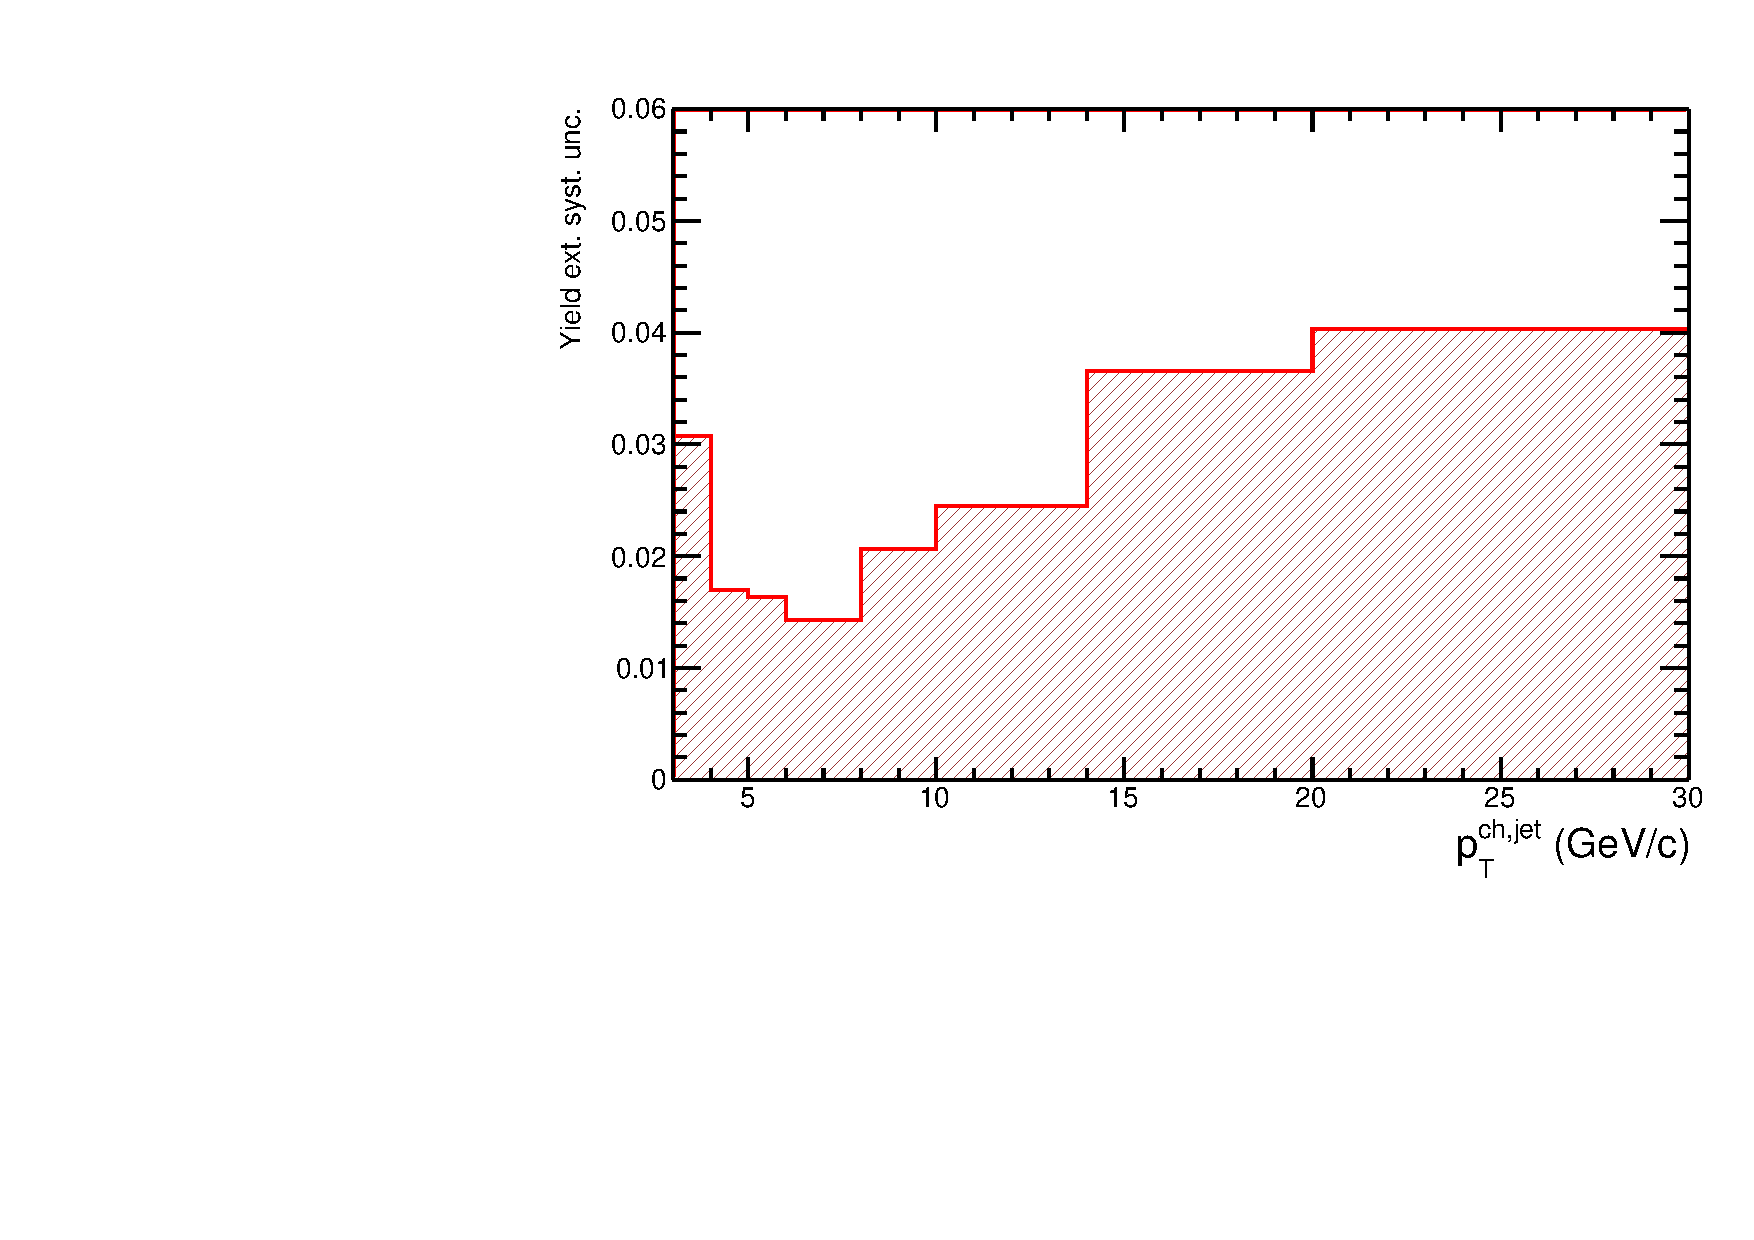
\includegraphics[width=0.5\textwidth]{pPbplots/yieldExtraction/YieldExtSysUnc_SB}
\caption{The RMS of the multi-trial (systematic uncertainties).} 
\label{fig:MultiTrialRMS_pPB}
\end{center}
\end{figure}

Figure~\ref{fig:MultiTrialSB_trials_pPB} shows average of the multi-trial procedure for the side-band method as a function of jet \pt\ for each \Dstar\ \pt\ bin scaled by the corresponding efficiency, and average of the all \Dstar \pt bins (blue). 
%And the Fig.~\ref{fig:MultiTrialSB_alltrials_pPB} presents variations of all considered trials, as a function of jet \pt .
%Variations of all trials as a function of jet \pt\ for each \Dstar\ \pt\ bin and scaled by the corresponding efficiency are shown in Fig~\ref{fig:MultiTrialSB_allDptVairations_pPB}.

\begin{figure}[bth]
\begin{center}
\begin{subfigure}[b]{.45\textwidth}
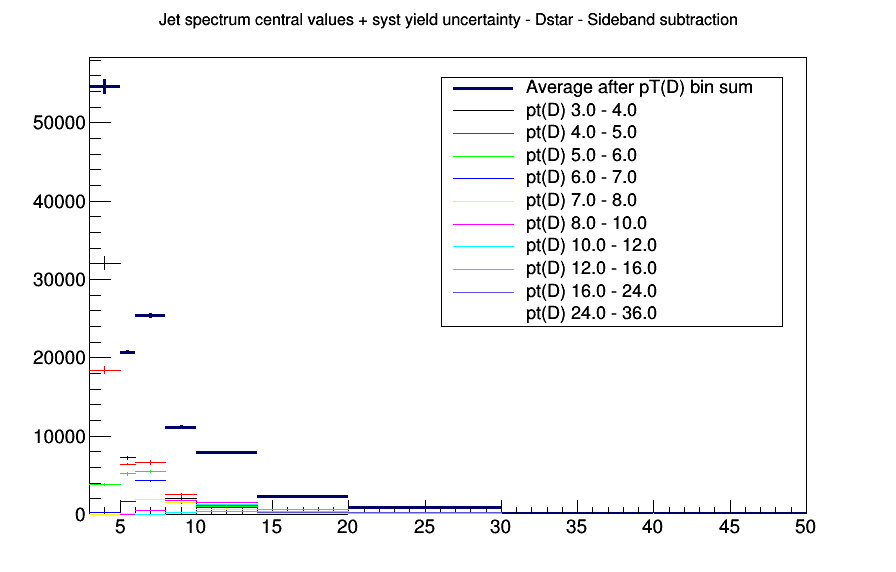
\includegraphics[width=\textwidth]{pPbplots/yieldExtraction/yieldInDbins}
\end{subfigure}
\begin{subfigure}[b]{.45\textwidth}
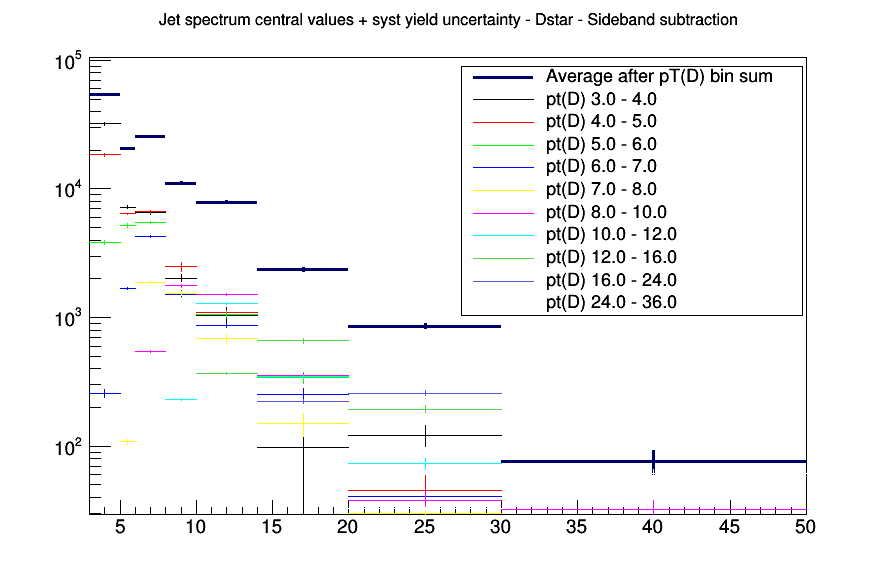
\includegraphics[width=\textwidth]{pPbplots/yieldExtraction/yieldInDbins_log}
\end{subfigure}
\caption{Average of the multi-trial procedure for the side-band method as a function of jet \pt\ for each \Dstar\ \pt\ bin scaled by the corresponding efficiency, and average of the all \Dstar \pt bins (blue).} 
\label{fig:MultiTrialSB_trials_pPB}
\end{center}
\end{figure}

\subsection{D-Meson Selection Cuts}
Uncertainties of the D-meson cut selection is estimated by varying applied in the analysis D-meson selection criteria, as reported in~\ref{sec:DmesonSel}. Four variations are considered, two looser sets and two tighter sets of cuts with $\pm$10\% and $\pm$15\% variation from a default cut value. Raw \Dstar-jet \pt\ distributions with these different cut sets and corresponding \Dstar-jet efficiencies are shown in Fig.~\ref{fig:JetPtRawSys}, and ratios in Fig.~\ref{fig:JetPtRawSysRatio}. Figure

\begin{figure}[bth]
\begin{center}
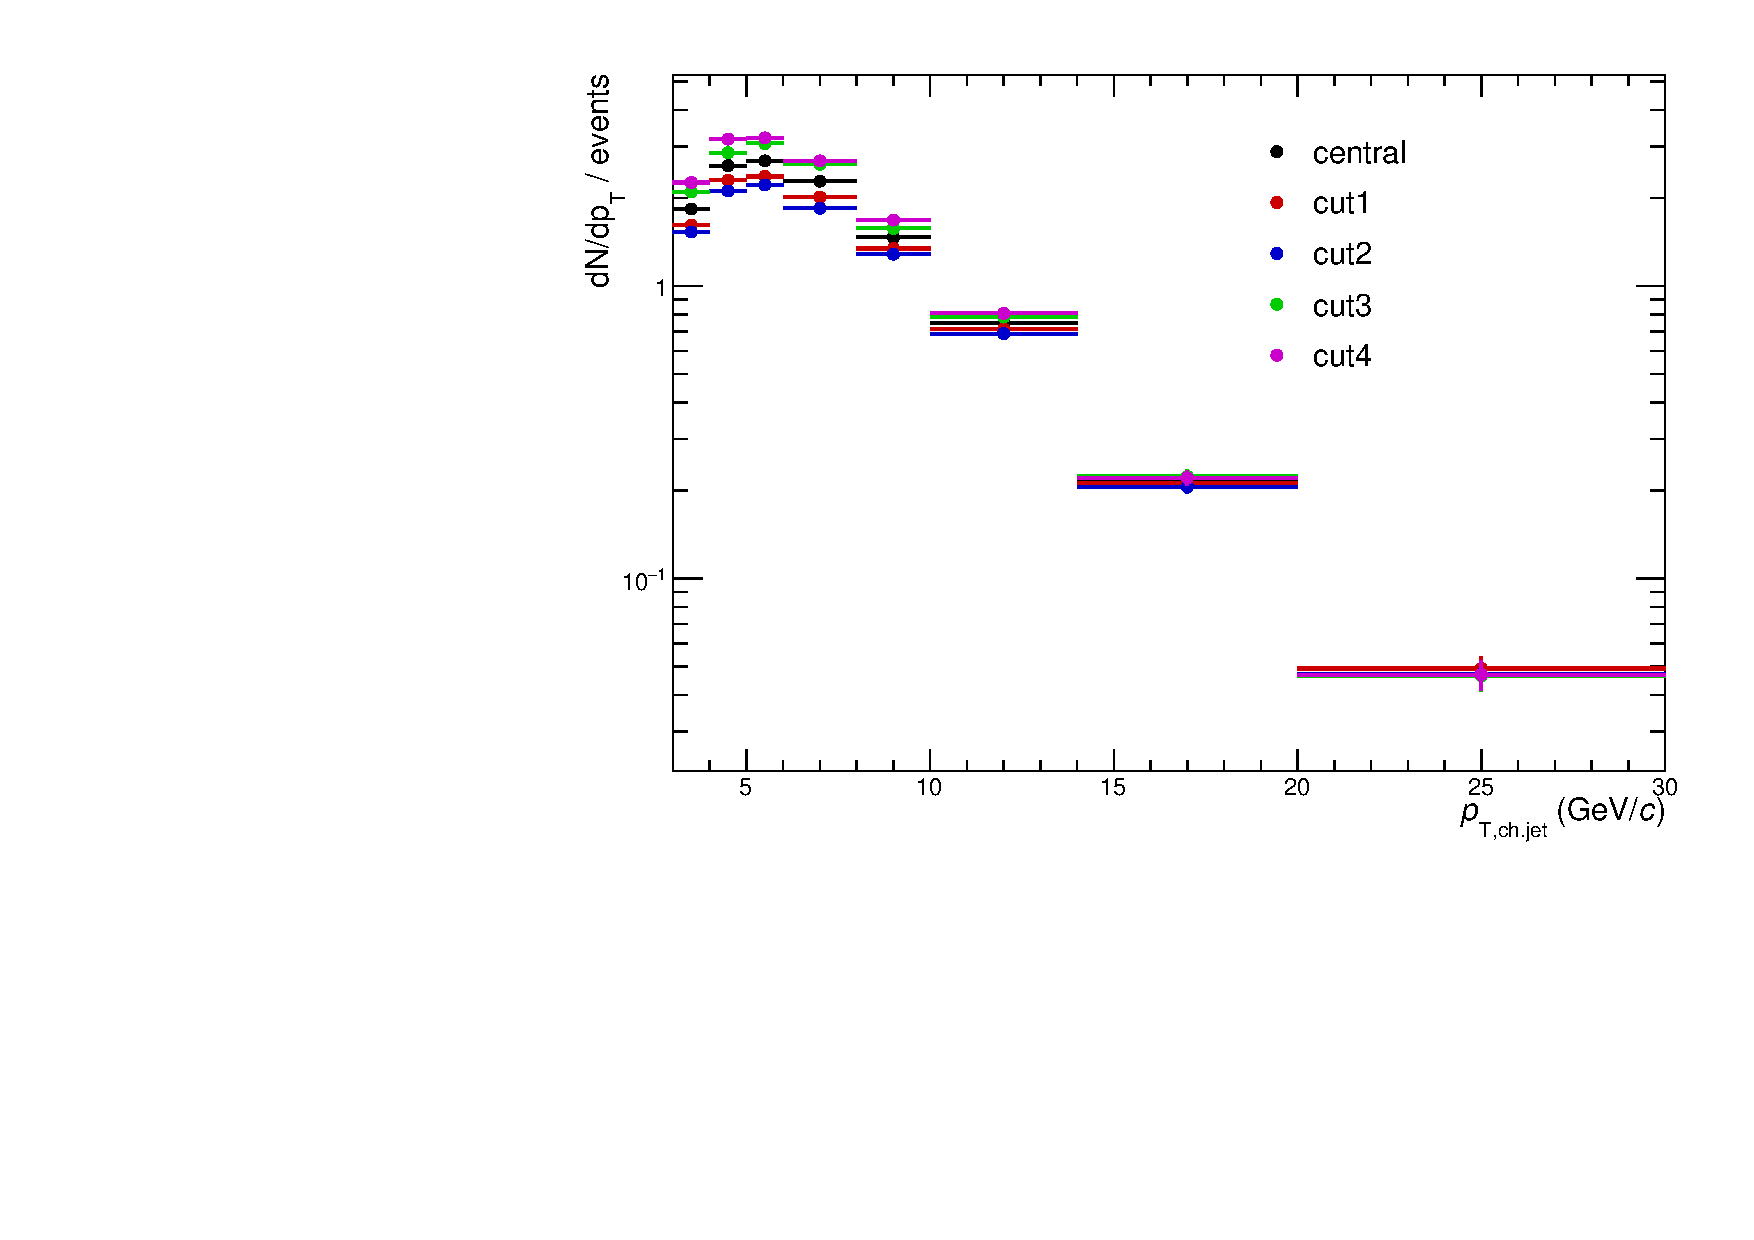
\includegraphics[width=0.49\textwidth]{pPbplots/jetSpectra/jetRawSpectra_pTD_pTD3}
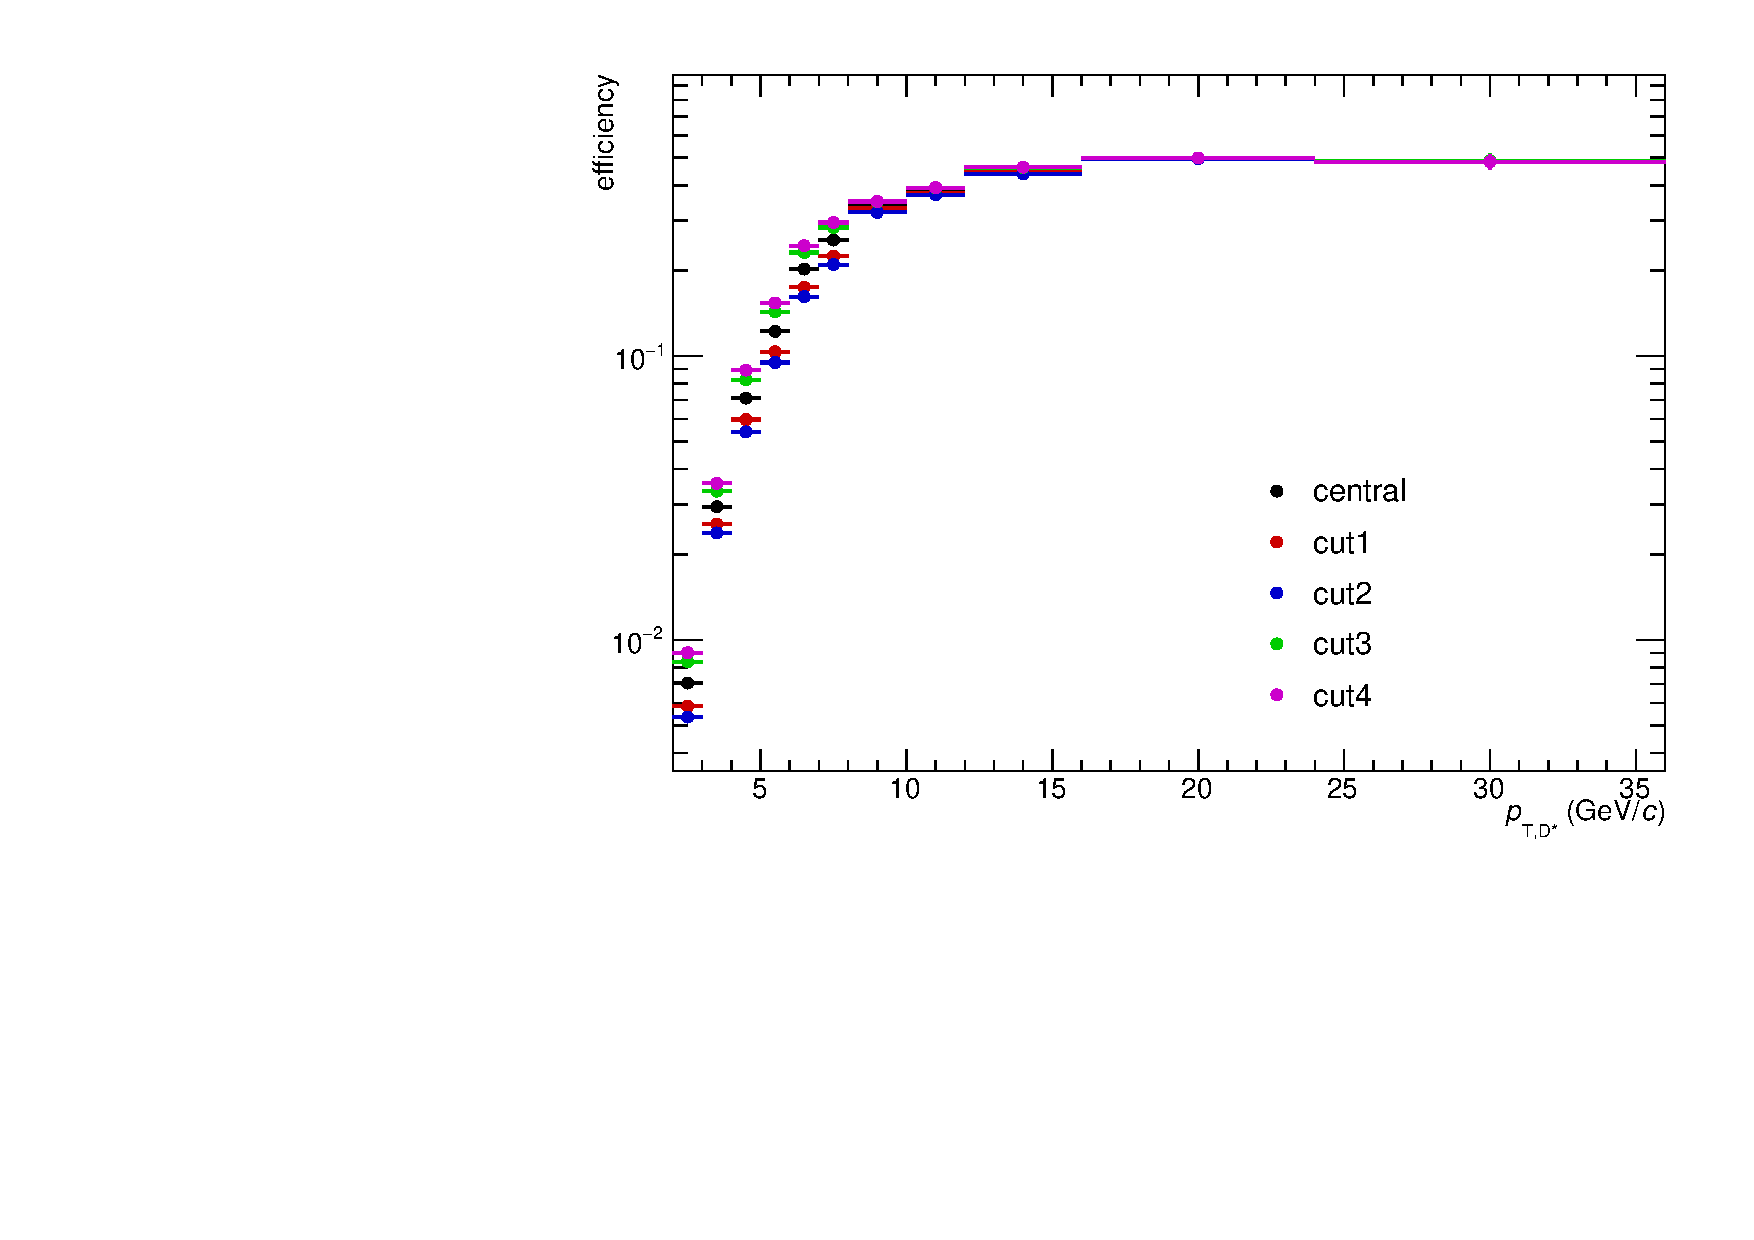
\includegraphics[width=0.49\textwidth]{pPbplots/jetSpectra/efficiencies}
\caption{Left: \Dstar-jet \pt\ distributions with different cut sets for systematic uncertainties estimation. Right: corresponding \Dstar-jet efficiencies.} 
\label{fig:JetPtRawSys}
\end{center}
\end{figure}

\begin{figure}[bth]
\begin{center}
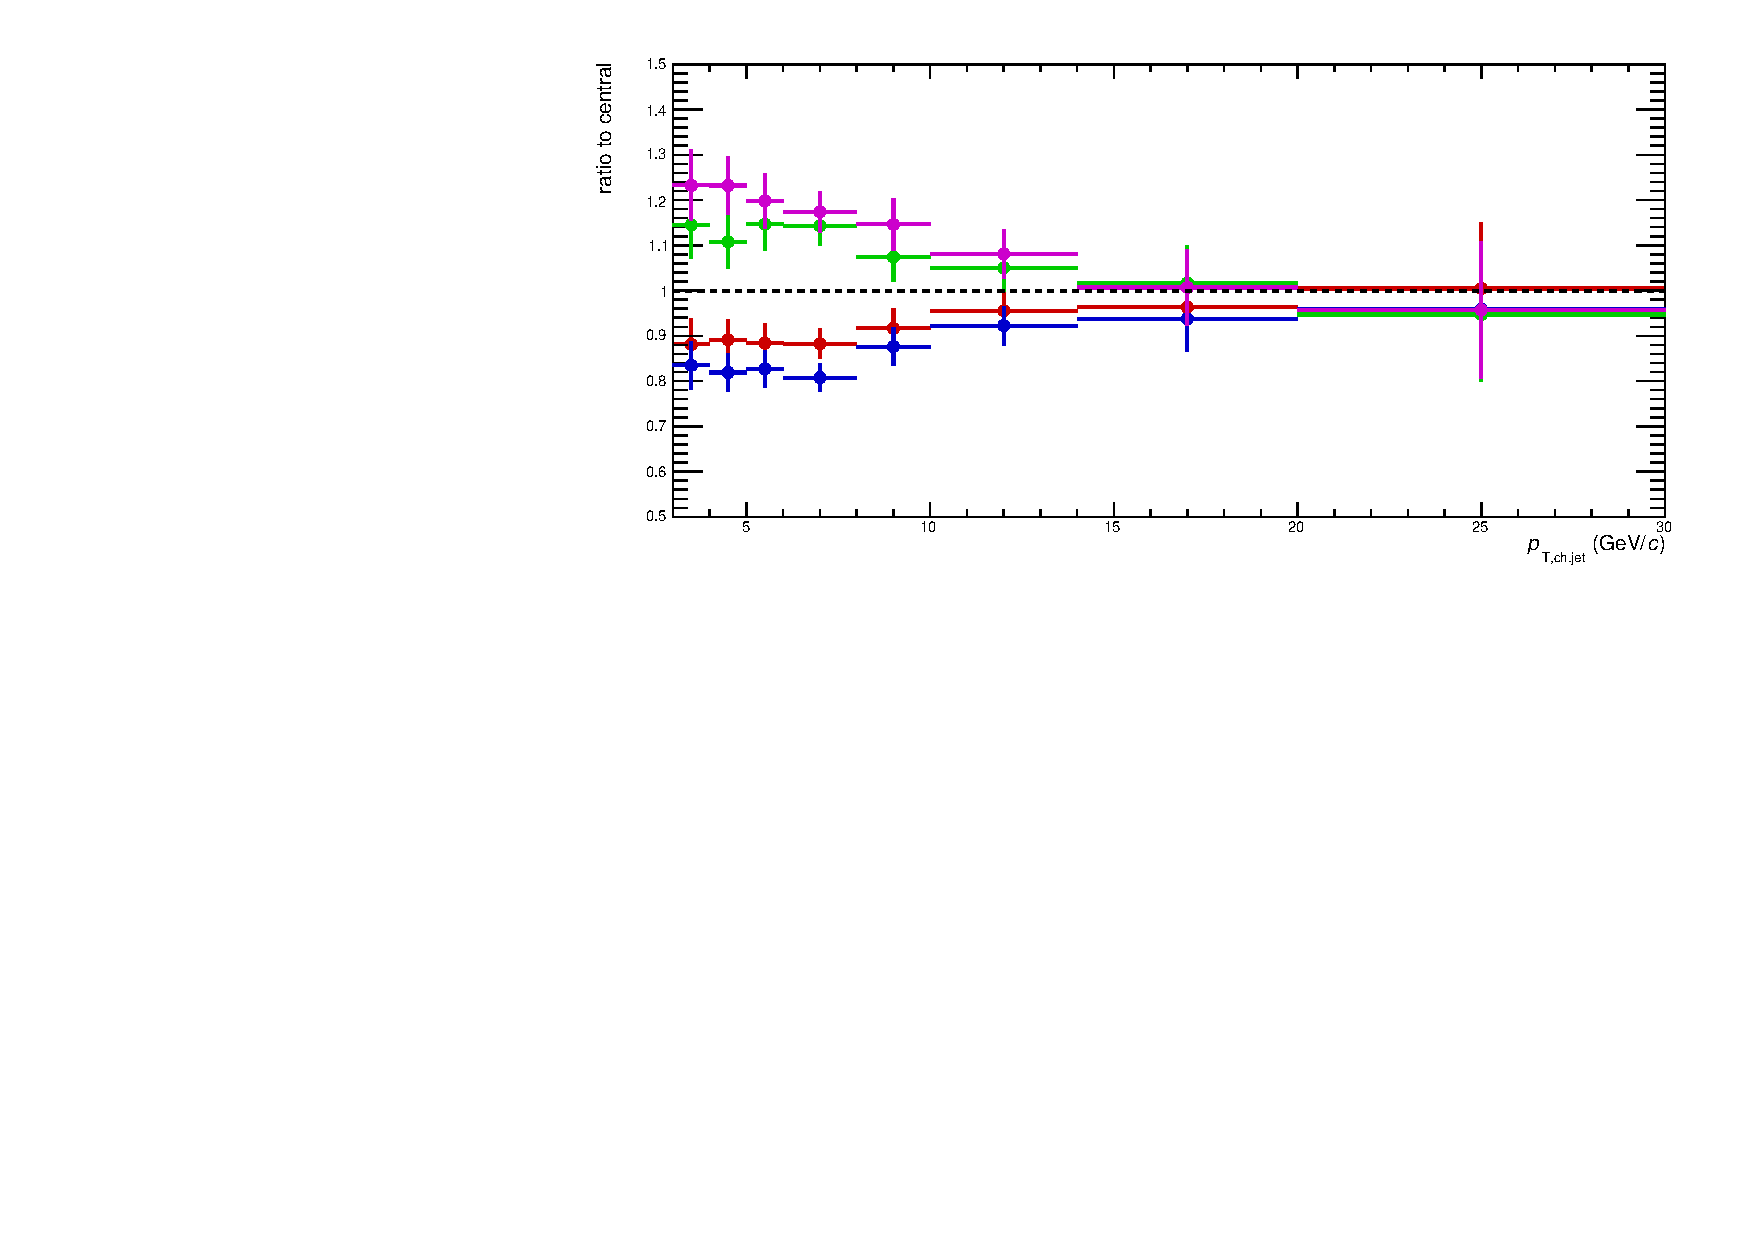
\includegraphics[width=0.49\textwidth]{pPbplots/jetSpectra/jetRawSpectraRatio_pTD_pTD3}
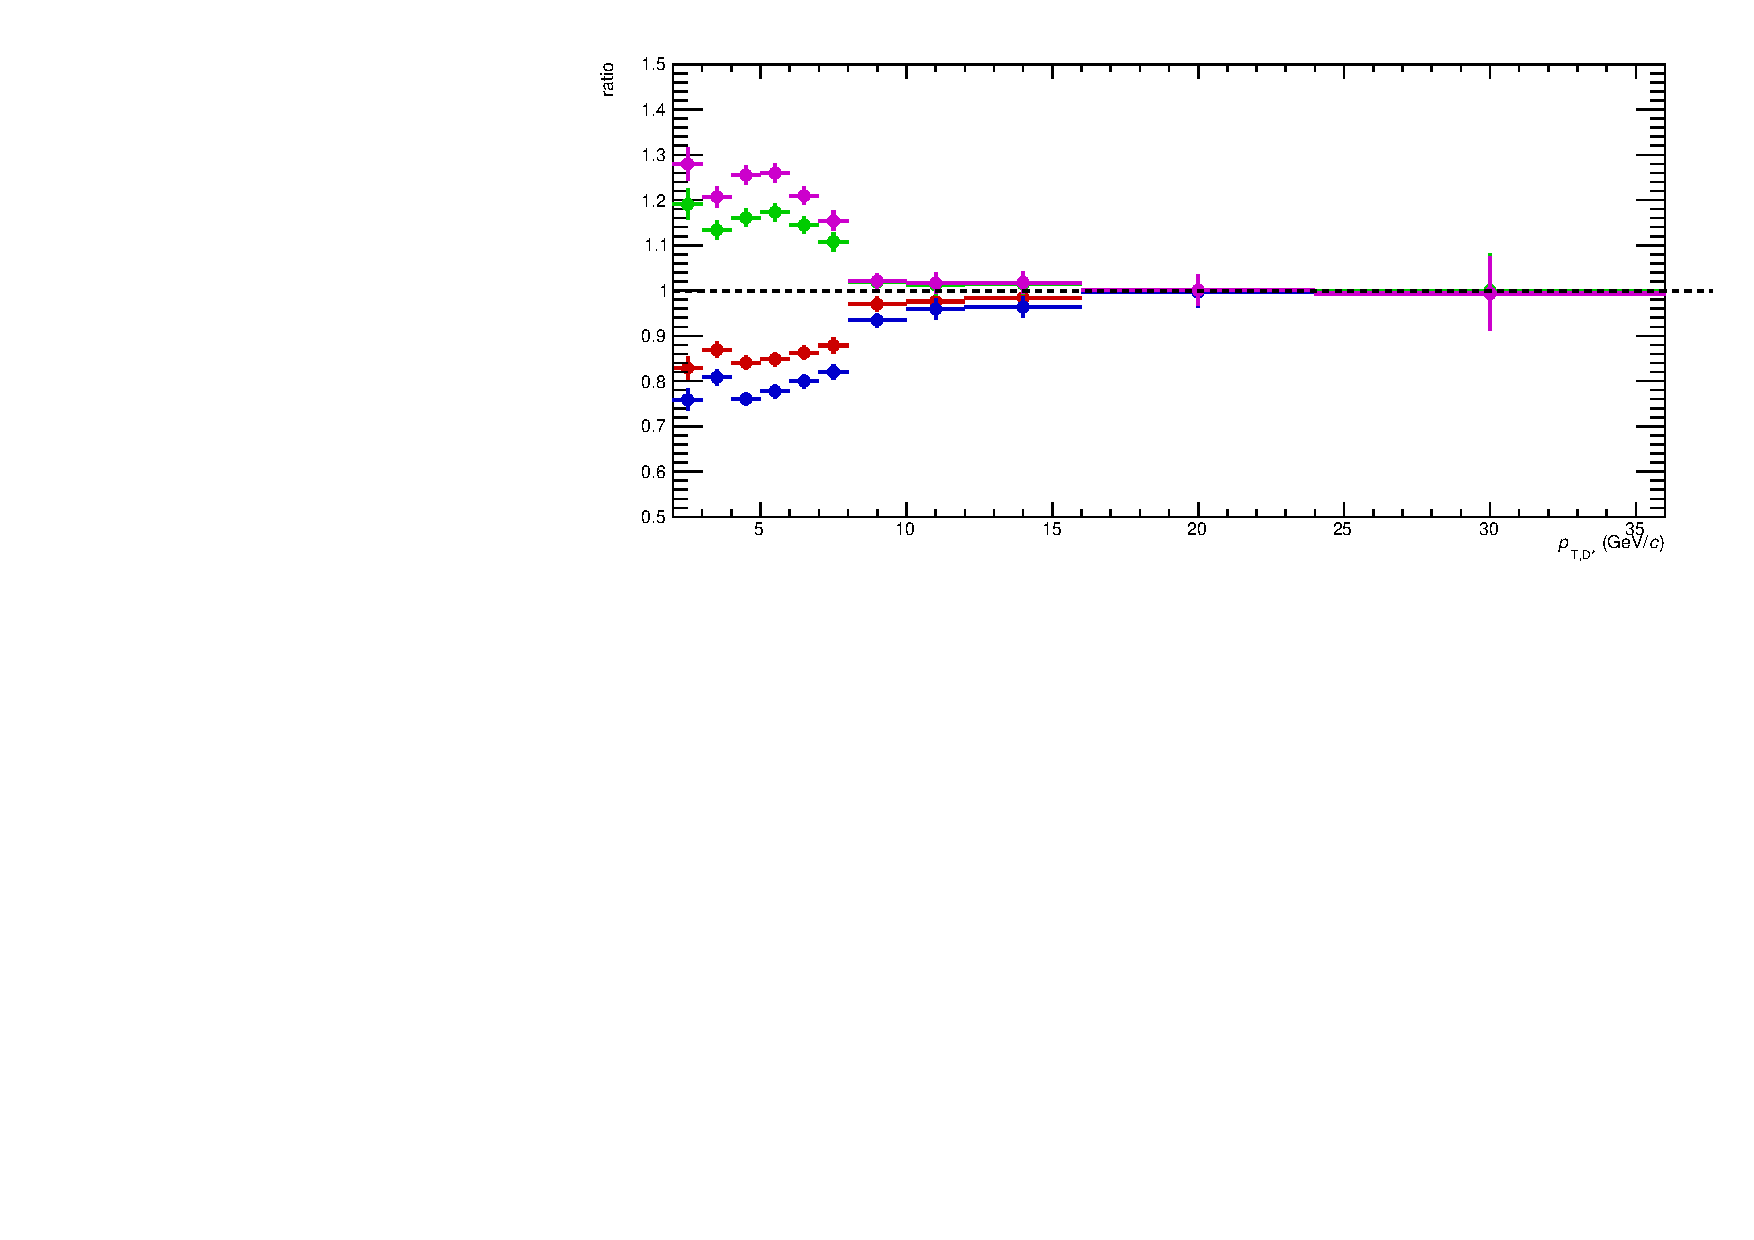
\includegraphics[width=0.49\textwidth]{pPbplots/jetSpectra/efficienciesRatio}
\caption{Left: Ratios of \Dstar-jet \pt\ distributions with different cut sets for systematic uncertainties estimation. Right: ratios of the corresponding \Dstar-jet efficiencies.} 
\label{fig:JetPtRawSysRatio}
\end{center}
\end{figure}

Corrected for the corresponding efficiency \Dstar-jet \pt\ distributions are presented in Fig.~\ref{fig:JetPtSys}. Systematic uncertainties are estimated by taking ratio of the efficiency-corrected \Dstar-jet \pt\ distributions with different cut variations to the \Dstar-jet \pt\ spectrum obtained with the default cut set and taking RMS of them, as shown in Fig

\begin{figure}[bth]
\begin{center}
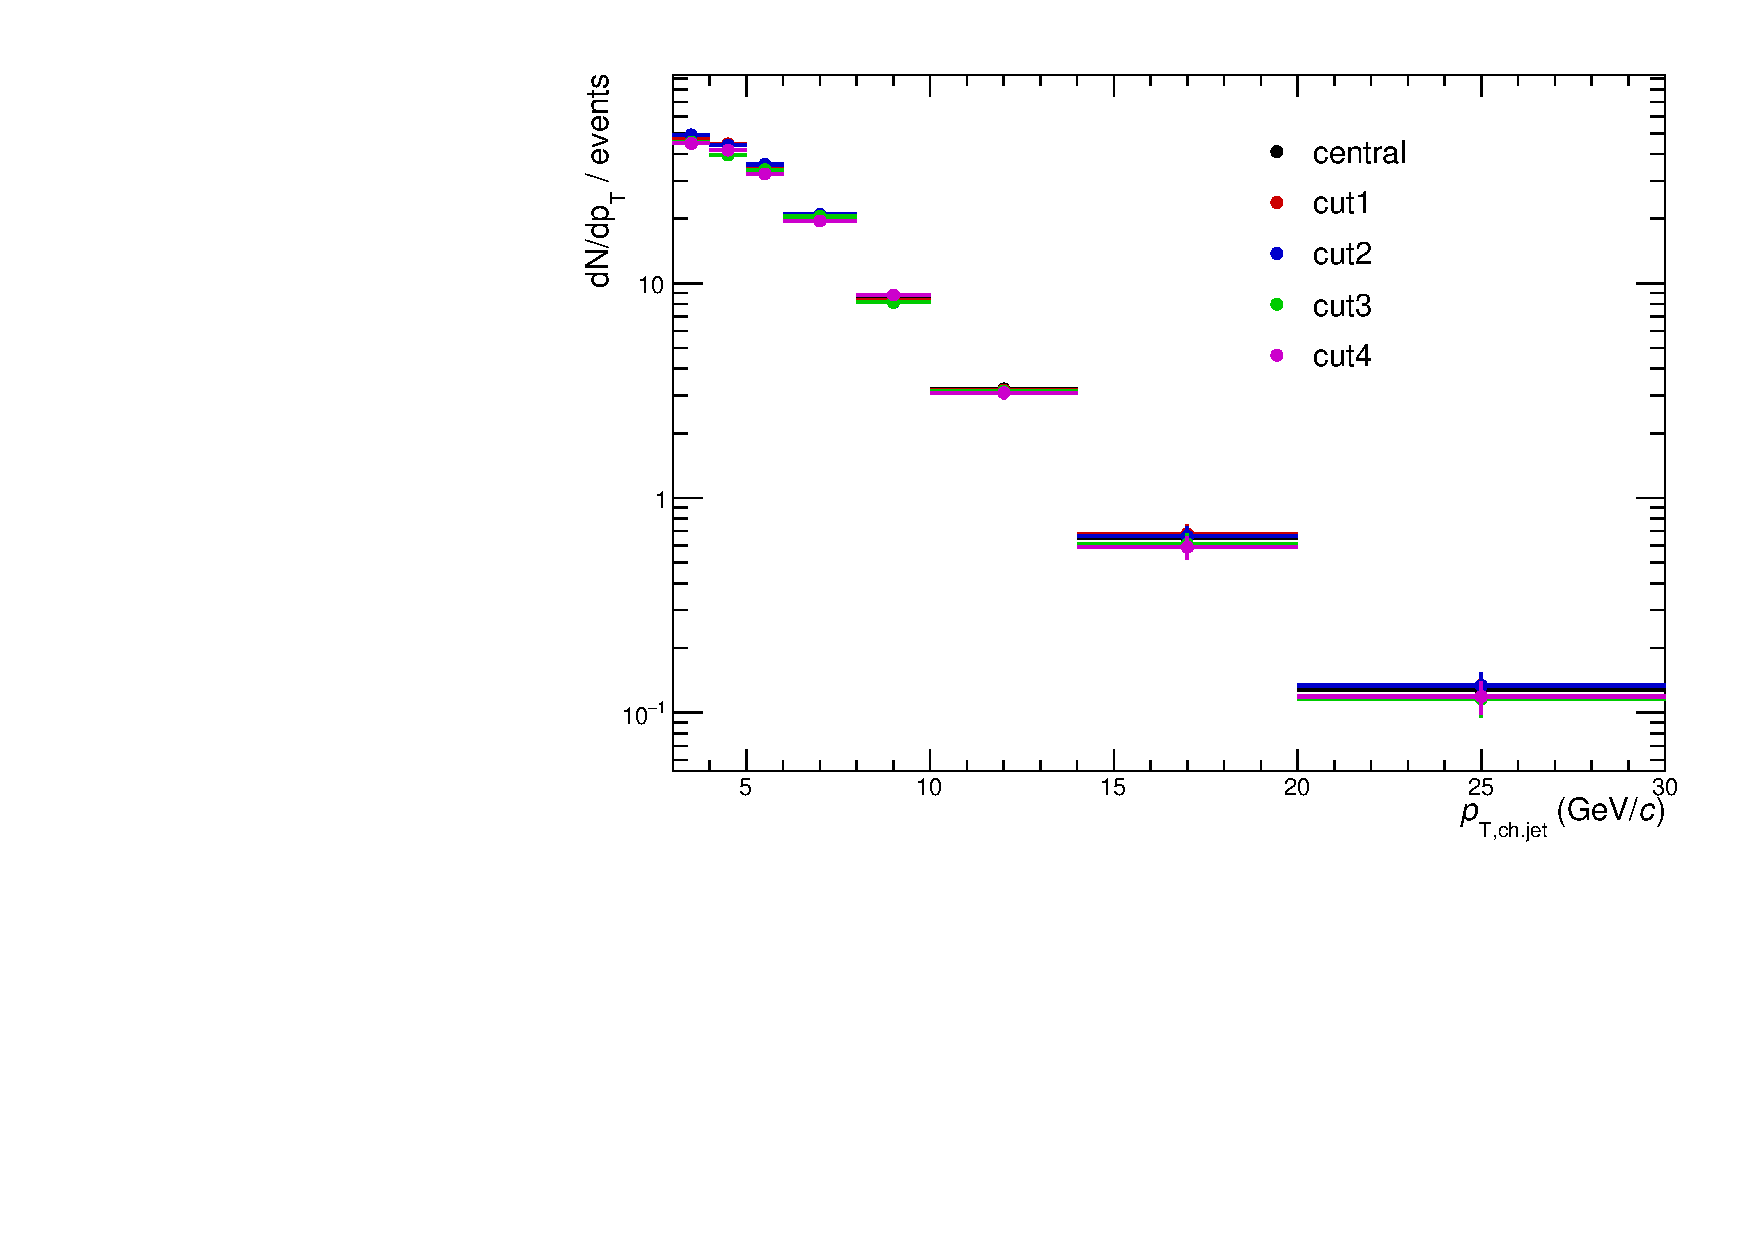
\includegraphics[width=0.49\textwidth]{pPbplots/jetSpectra/jetSpectra_pTD_pTD3}
\caption{Efficiency-corrected \Dstar-jet \pt\ distributions with different cut sets for systematic uncertainties estimation.} 
\label{fig:JetPtSys}
\end{center}
\end{figure}

\begin{figure}[bth]
\begin{center}
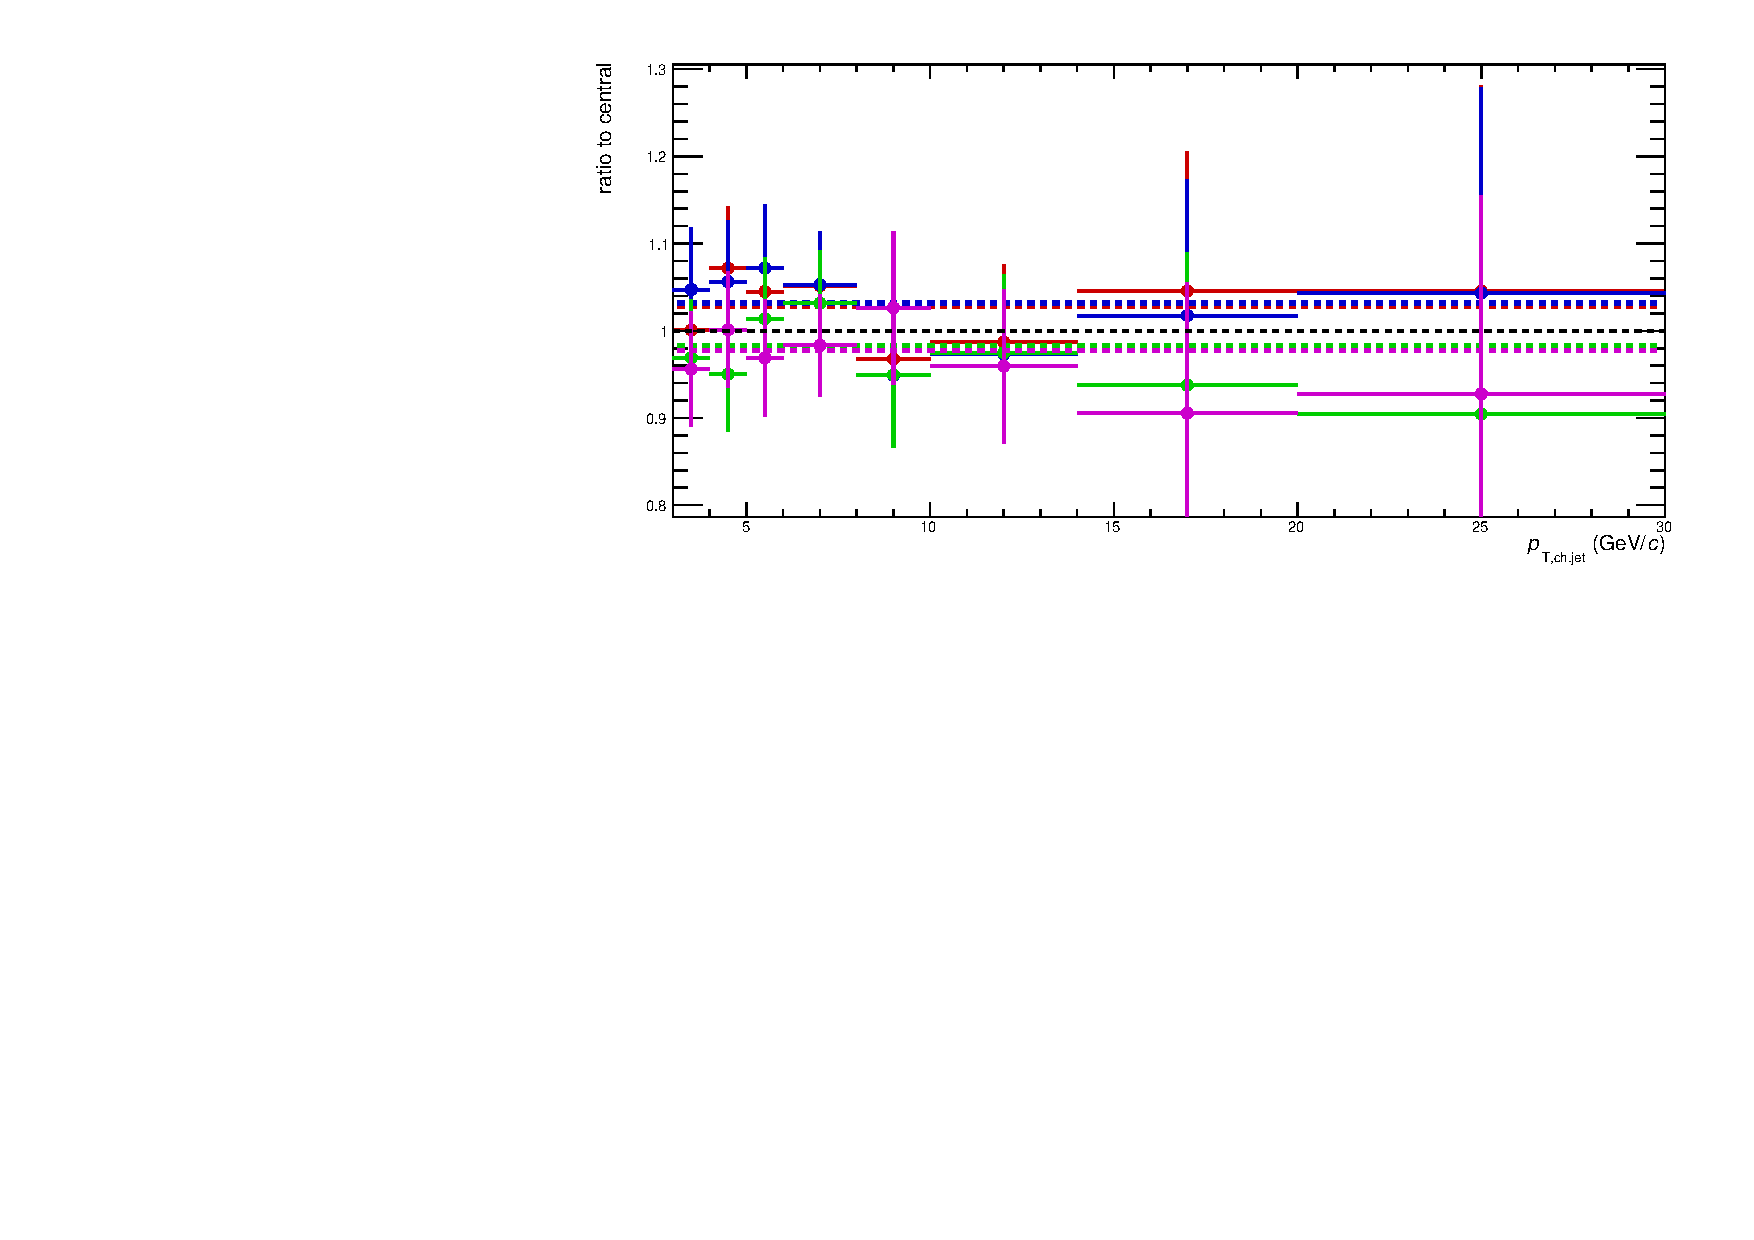
\includegraphics[width=0.49\textwidth]{pPbplots/jetSpectra/jetSpectraRatio_pTD_pTD3}
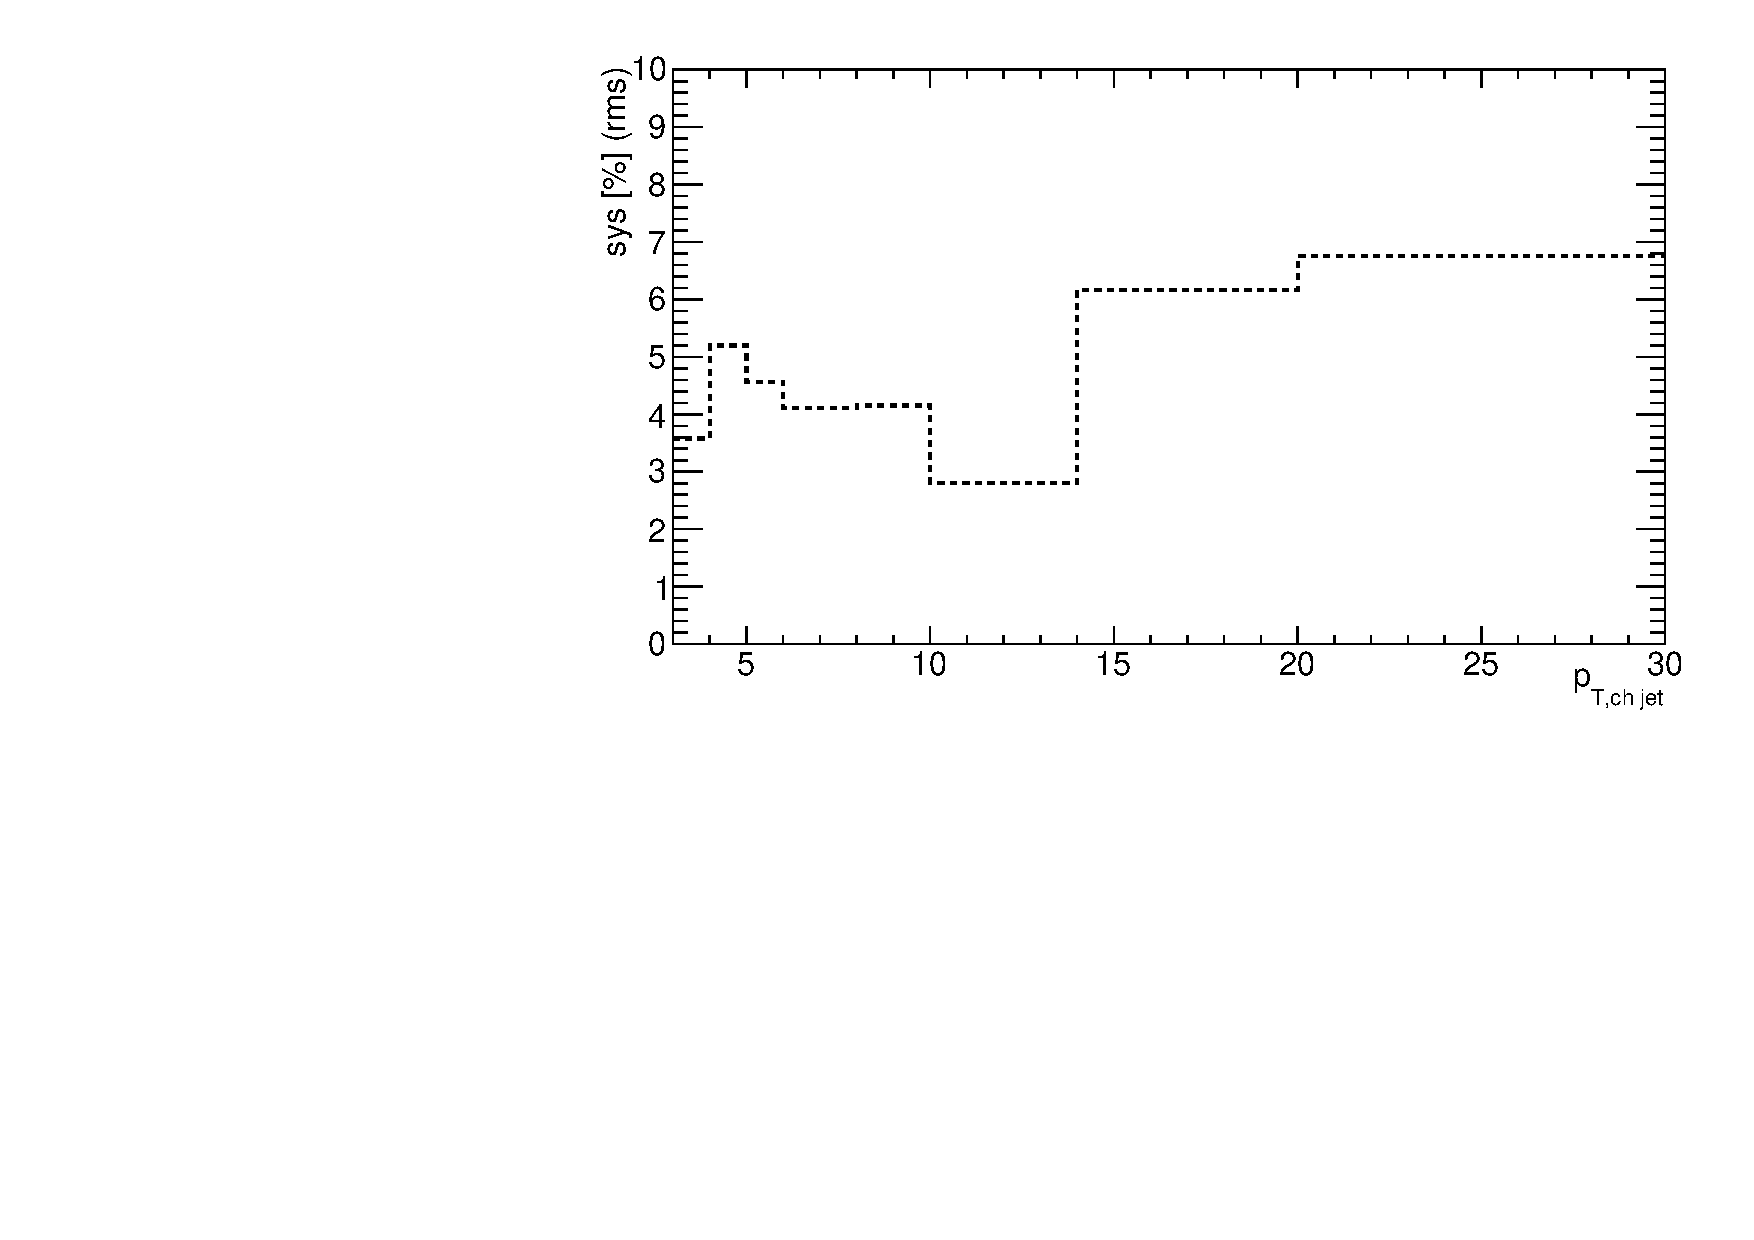
\includegraphics[width=0.49\textwidth]{pPbplots/jetSpectra/jetSpectraSys_pTD_pTD3}
\caption{Left: Ratio of the efficiency-corrected \Dstar-jet \pt\ distributions with different cut sets for systematic uncertainties estimation. Right: RMS - systematic uncertainties.} 
\label{fig:JetPtSys}
\end{center}
\end{figure}


\subsection{B Feed-Down Correction}

The B Feed-Down (FD) cross section is obtained from a POWHEG+PYTHIA6 simulation, as discussed in Section~\ref{sect:FD}.
In order to assess the systematic uncertainty the same simulation is performed with different choices of the quark mass $m_{\rm b}$, the factorization scale factor $\mu_{\rm F}$, and the renormalization scale factor $\mu_{\rm R}$.
Table~\ref{tab:FDpars} shows the list of parameters used to determine the central points and the variations used to determine the systematic uncertainty.


\begin{table}[bth]
\caption{Parameters of the POWHEG+PYTHIA6 simulations used to estimate the B Feed-Down.}
     \label{tab:FDpars}
\begin{center}
    \begin{tabular}{lrr}
    \hline
    Parameter & Central Value & Variations \\ \hline
    $m_{\rm b}$ & $4.75$~\GeVcsq & $4.5$, $5.0$~\GeVcsq \\ 
    PDF & CT10nlo (11000) & -- \\ 
    nPDF & EPS09nlo & -- \\
    ($\mu_{\rm F}$, $\mu_{\rm R}$) & (1,1) & (0.5,0.5), (0.5, 1), (1, 0.5), (2,2), (2,1), (1,2)
    \end{tabular}
    \end{center}
    \end{table}

Figures~\ref{fig:BFeedDown_DPtSpectrum_GeneratorLevel_DPtSpectrum} and~\ref{fig:BFeedDown_DPtSpectrum_GeneratorLevel_JetSpectrum} compare the cross sections obtained with the various choices of parameters listed in Table~\ref{tab:FDpars}, respectively as a function of \ptd\ and \ptchjet. %The most extreme variations differ up to 20-30\% from the central points.
The \ptchjet\ distribution is with the analysis cut on \ptd\: 3-36 GeV/$c$, and scaled by non-prompt to prompt efficiency ratio.

\begin{figure}[bth]
\begin{center}
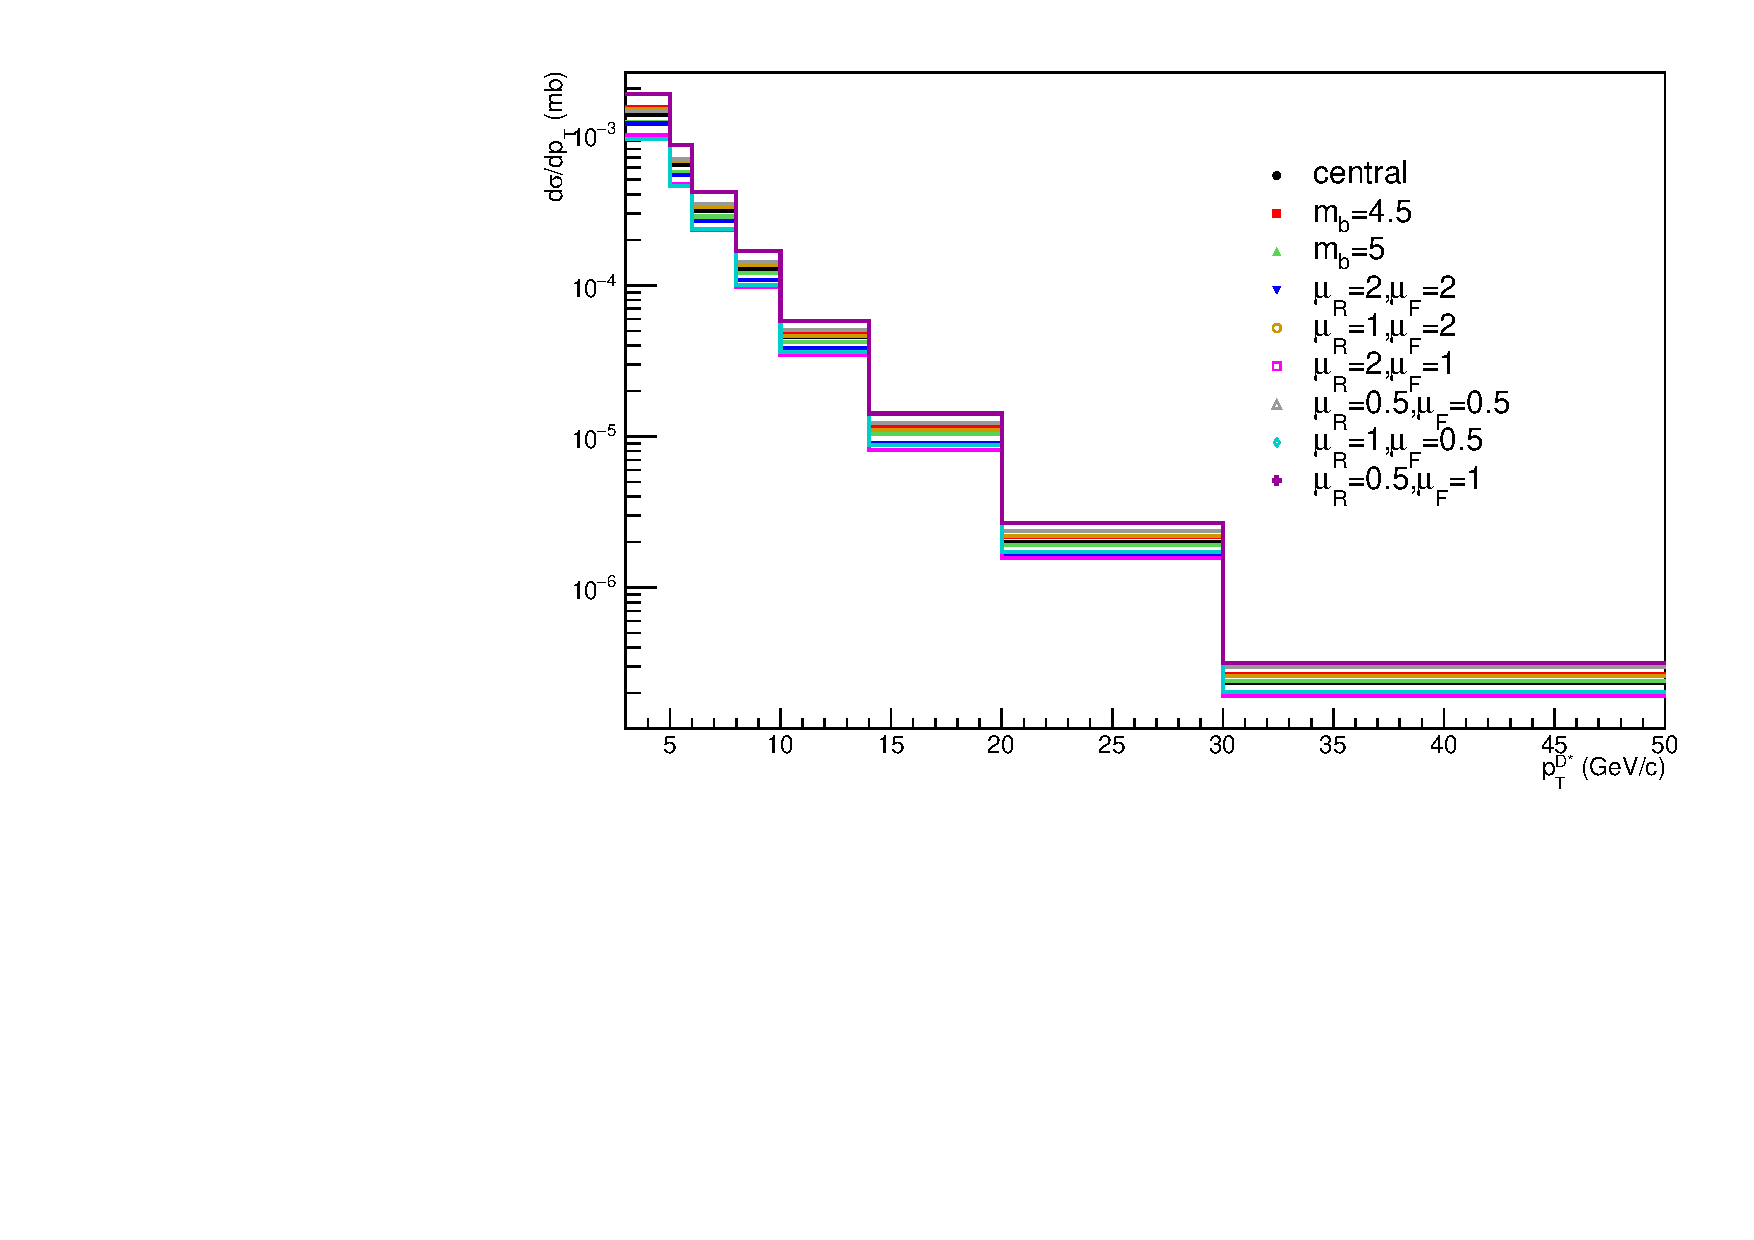
\includegraphics[width=.45\textwidth]{pPbplots/simulations/NonPromptspectra_DPt}
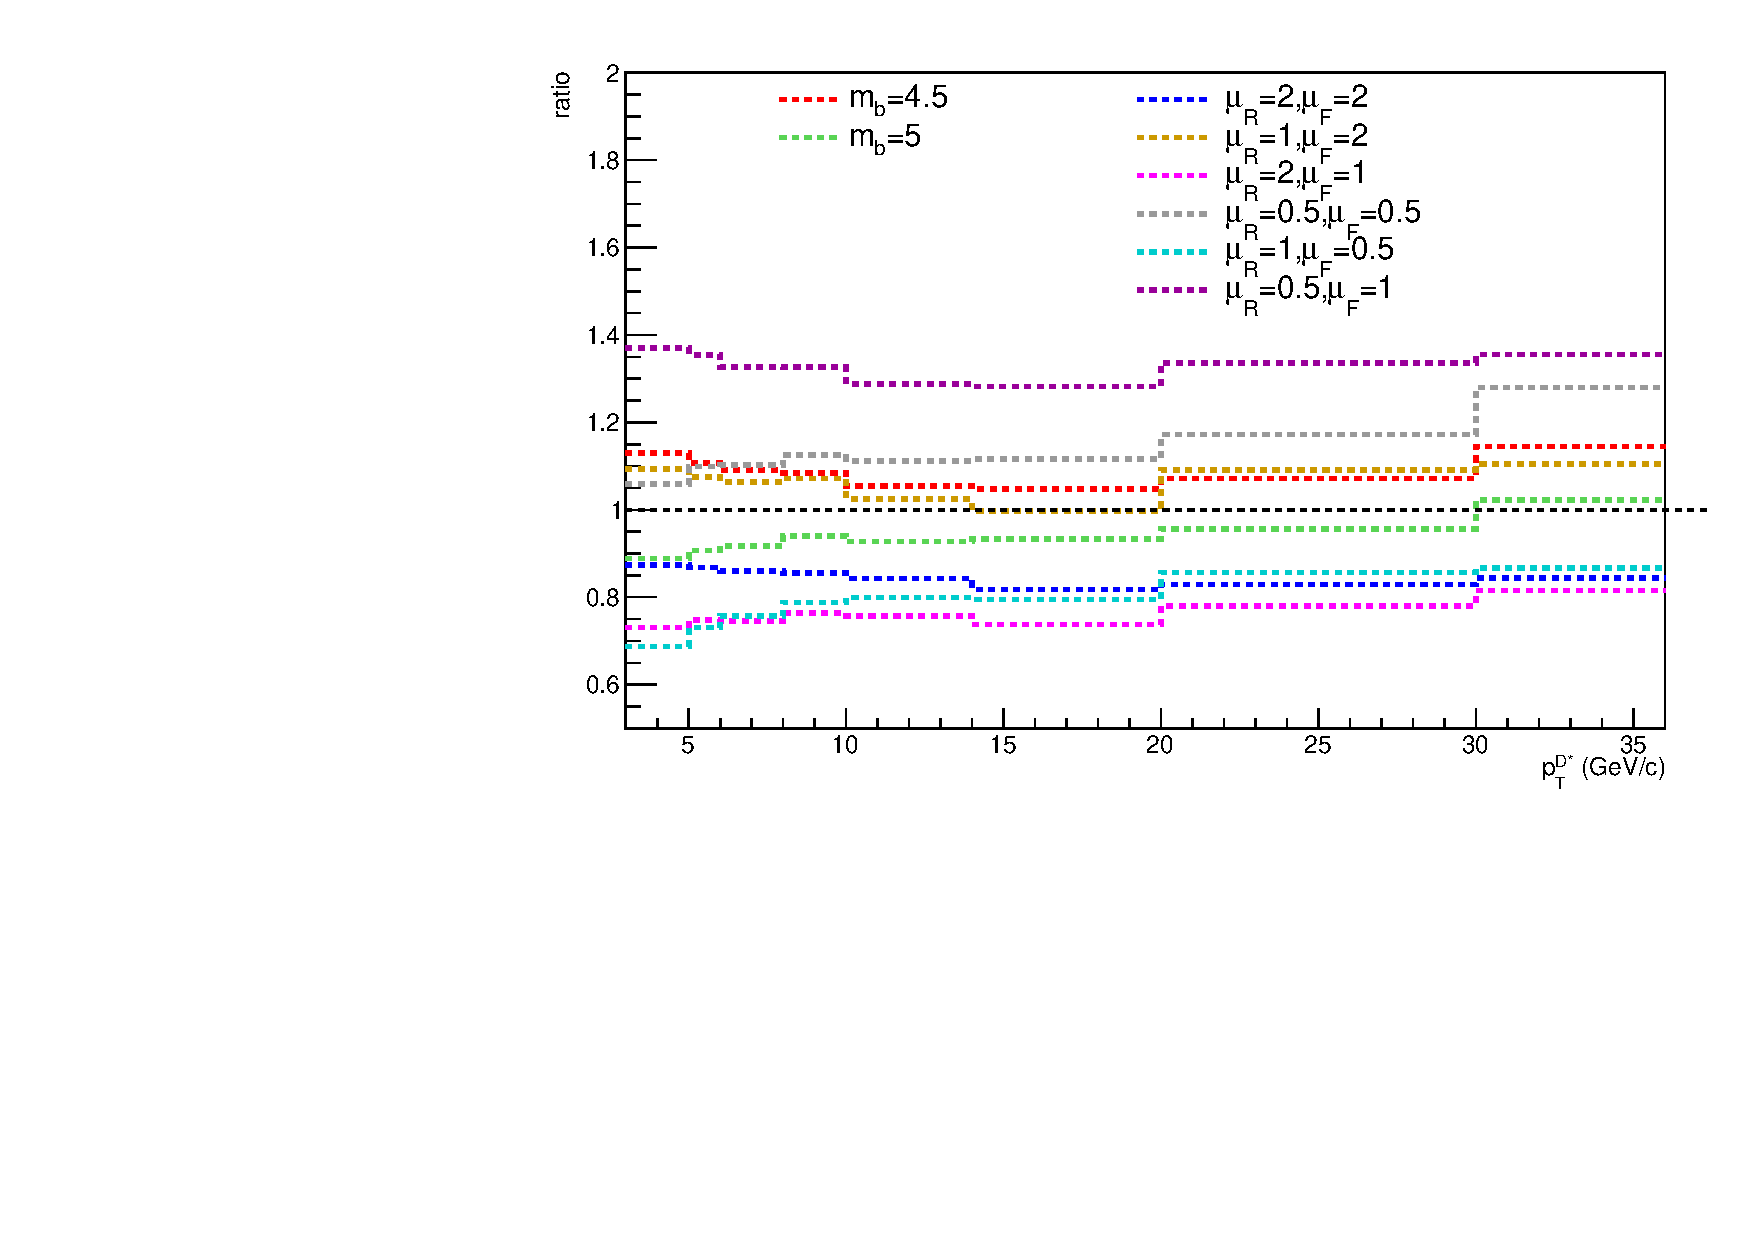
\includegraphics[width=.45\textwidth]{pPbplots/simulations/NonPromptspectra_DPt_ratio}
\caption{Non-prompt (B Feed-Down) \Dstar-jet cross section in \pPb\ at $\snn=5.02$~TeV as a function of \ptd, obtained in POWHEG+PYTHIA6 simulations with different choices of the simulation parameters.} 
\label{fig:BFeedDown_DPtSpectrum_GeneratorLevel_DPtSpectrum}
\end{center}
\end{figure}

\begin{figure}[bth]
\begin{center}
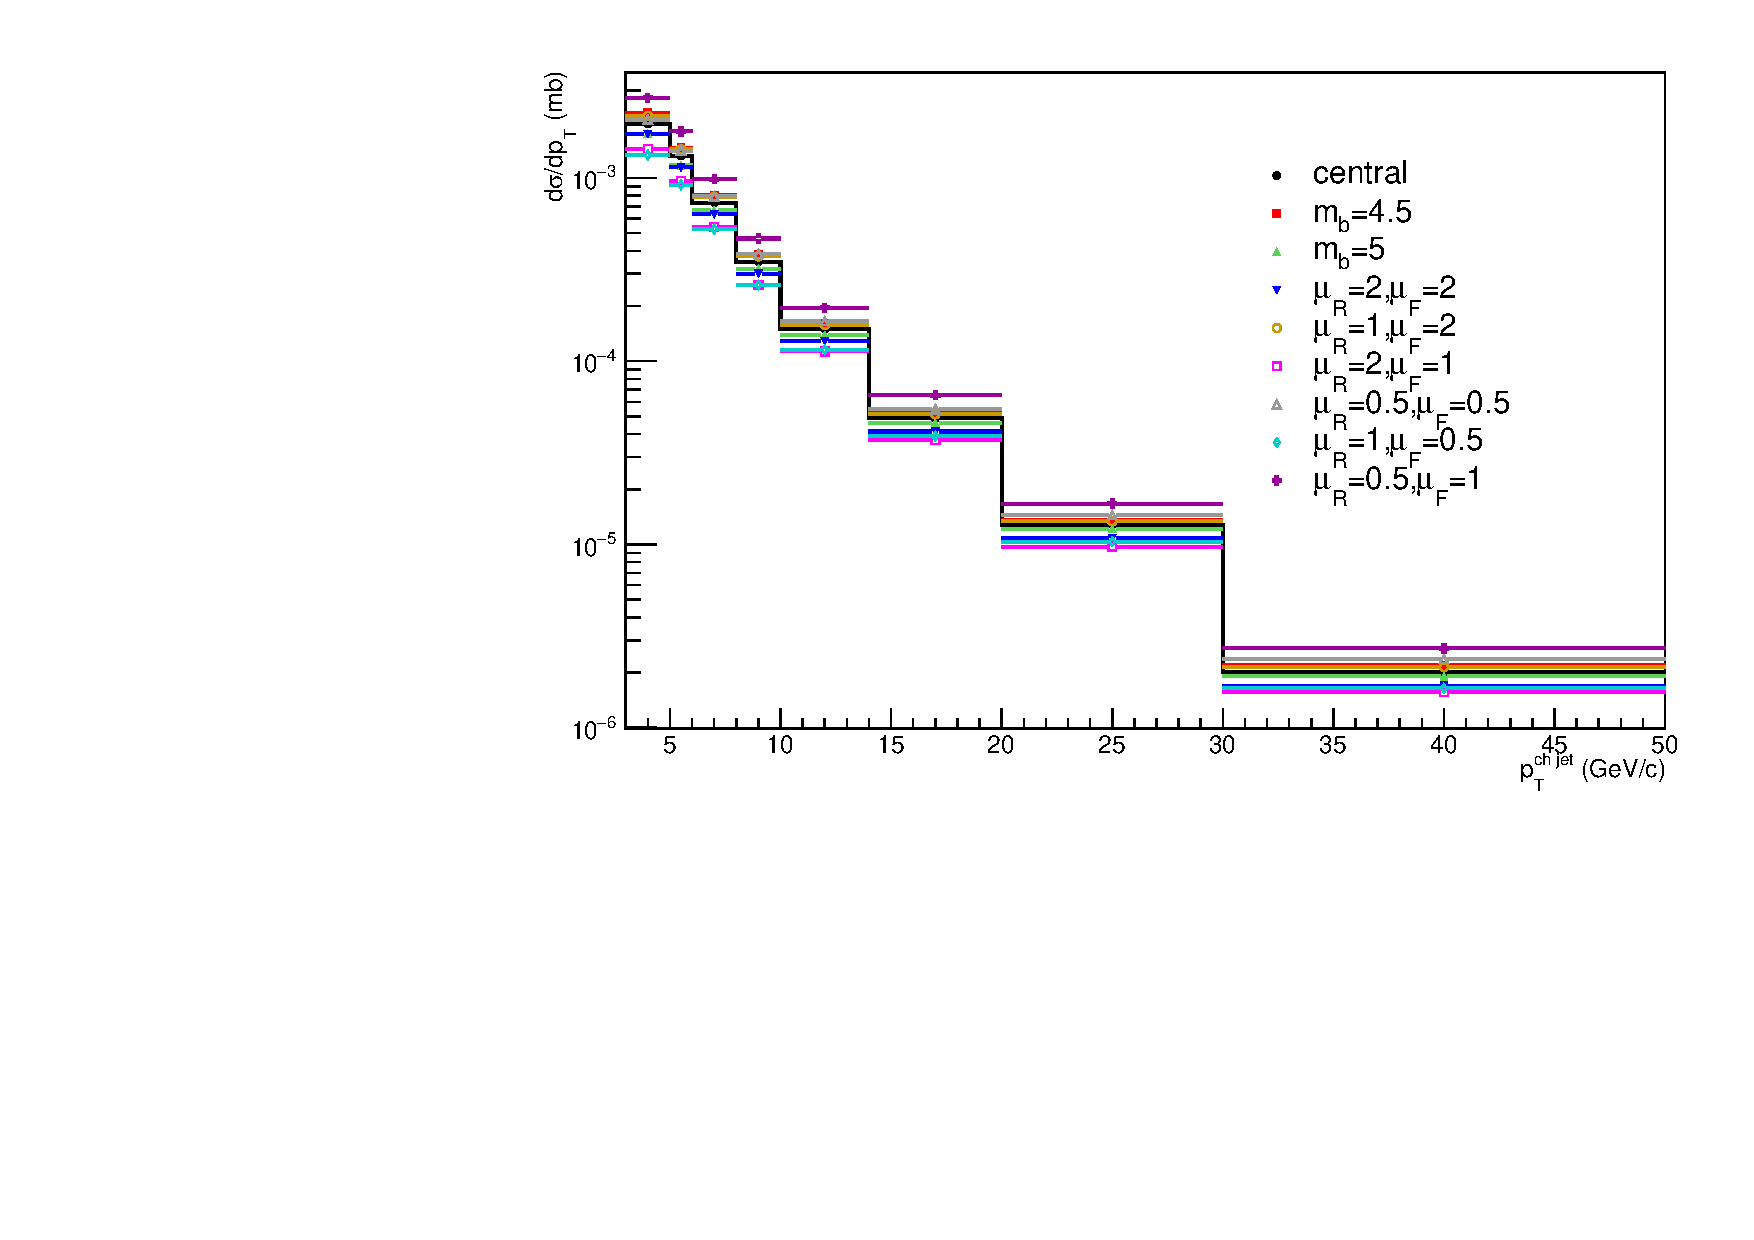
\includegraphics[width=.45\textwidth]{pPbplots/simulations/NonPromptspectra_JetPt_Dpt3_36_effScaled}
\includegraphics[width=.45\textwidth]{pPbplots/simulations/NonPromptspectra_JetPt_Dpt3_36_effScaled_ratio}
\caption{Non-prompt (B Feed-Down) \Dstar-jet cross section in \pPb\ at $\snn=5.02$~TeV as a function of \ptchjet, obtained in POWHEG+PYTHIA6 simulations
with different choices of the simulation parameters, \ptd\: 3-36 GeV/$c$.} 
\label{fig:BFeedDown_DPtSpectrum_GeneratorLevel_JetSpectrum}
\end{center}
\end{figure}

Figures~\ref{fig:BFeedDown_GeneratorLevel_Spectrum_canvas} shows the final differential cross sections as a function of \ptchjet\ with systematic uncertainties. The systematic uncertainties are obtained by taking the largest upward and downward variation from the central point in each bin. In this Figure uncertainties are therefore asymmetric. For the FD subtraction the largest between the upward and downward uncertainty is used in order to have a symmetric uncertainty.

\begin{figure}[bth]
\begin{center}
\includegraphics[width=.45\textwidth]{pPbplots/simulations/NonPromptspectra_JetPt_Dpt3_36_effScaled_un}
\includegraphics[width=.45\textwidth]{pPbplots/jetSpectra/FDUnc_beforeUnf}
\caption{Left: Non-prompt (B Feed-Down) \Dstar-jet cross section in \pPb\ at $\snn=5.02$~TeV, obtained in a POWHEG+PYTHIA6 simulation with the systematic uncertainty. Right: Final systematic uncertainties after the B feed-down subtraction from the inclusive \Dstar-jet spectrum. } 
\label{fig:BFeedDown_GeneratorLevel_Spectrum_canvas}
\end{center}
\end{figure}


\subsection{Unfolding}
\label{sUnfoldSys}


Figure~\ref{fig:unfBayesReg_pPb} shows how the unfolded  \Dstar-jet\ spectrum in \pPb\ collisions evolves with increasing number of iterations, and ratios of folded spectra with different iterations to the default iteration.
Fig.~\ref{fig:unfSVDReg_pPb} presents unfolded jet spectrum from the SVD method~\cite{Hocker:1995} on the left, and the right plot shows ratio of folded to measured spectra with different iterations.
For the systematic uncertainty estimation also priors used for unfolding are varied. The baseline prior used for unfolding is the spectrum obtained (at generator level) from PYTHIA.
For the variations, the spectra were obtained from a modified power-law function:
\begin{equation}
f(\ptjet) = \ptjet^{-a}e^{-\frac{ab}{\ptjet}},
\end{equation}
where $a$ is the power-law index (we used two variations: $a=3,6$) and $b=3$~\GeVc\ is the position of the local maximum of the distribution. The exponential factor $e^{-\frac{ab}{\ptjet}}$ was added
to avoid infinities at zero and have a more realistic spectrum (the physical cross-section goes to zero for $\ptjet \to 0$).

Figure~\ref{fig:unfcomparison} compares the unfolded results obtained starting from three different priors in the Bayesian iterative method: PYTHIA spectrum, modified power-law with indexes $3$ and $6$ with 5 iterations, in the Bayesian iterative method with 8 iterations, and unfolded spectrum obtained using SVD with 5 iterations. Figure~\ref{fig:unfcomparisonSys} presents ratio of these different unfolded spectra and RMS - systematic uncertainty.

\begin{figure}[bth]
\centering
\includegraphics[width=.45\textwidth]{pPbplots/unfolding/PythiaRM__Djet5Excl_2_bayes5_weight_unfSpectra}
\includegraphics[width=.45\textwidth]{pPbplots/unfolding/PythiaRM__Djet5Excl_2_bayes5_weight_unfRatio}
\caption{The evolution of the unfolded spectra with increasing number of iterations for the Bayesian method is shown in different colors.
The ratios between each number-of-iteration choices and the baseline (5 iterations) are shown on the right.}
\label{fig:unfBayesReg_pPb}
\end{figure}

\begin{figure}[bth]
\centering
\includegraphics[width=.45\textwidth]{pPbplots/unfolding/PythiaRM__Djet5Excl_SVD5_weight_UnfSpectrum}
\includegraphics[width=.45\textwidth]{pPbplots/unfolding/PythiaRM__Djet5Excl_SVD5_weight_foldedRatio}
\caption{The spectrum unfolded with the SVD method $k=$ 5 is shown on the left plot, and a comparison to the unfolded spectrum obtained using the Bayesian method is shown on the right.
The ratios between folded and measured spectrum for each number-of-iteration choices are shown on the right.}
\label{fig:unfSVDReg_pPb}
\end{figure}


\begin{figure}[bth]
\centering
\includegraphics[width=.45\textwidth]{pPbplots/unfolding/jetSpectra_unfSys}
\caption{Comparison of the unfolded results obtained starting from three different priors in the Bayesian iterative method: PYTHIA spectrum, modified power-law with indexes $3$ and $6$ with 5 iterations, in the Bayesian iterative method with 8 iterations, and unfolded spectrum obtained using SVD with 5 iterations.}
\label{fig:unfcomparison}
\end{figure}

\begin{figure}[bth]
\centering
\includegraphics[width=.45\textwidth]{pPbplots/unfolding/jetSpectraRatio_unfSys}
\includegraphics[width=.45\textwidth]{pPbplots/unfolding/jetSpectraSys_unfSys}
\caption{Left: Ratio of the unfolded results obtained starting from three different priors in the Bayesian iterative method: PYTHIA spectrum, modified power-law with indexes $3$ and $6$ with 5 iterations, in the Bayesian iterative method with 8 iterations, and unfolded spectrum obtained using SVD with 5 iterations. Right: RMS -- systematic uncertainty. }
\label{fig:unfcomparisonSys}
\end{figure}


\subsection{Background fluctuation matrix}

The background fluctuation matrix is determined in a data-driven way using the Random Cone method.
The default background fluctuation \deltapt\ is calculated using events that include D-jet candidates excluding the leading jet in an event, and with the leading jet $p_{T}>$ 5 GeV/$c$. For a systematic uncertainty estimation the \deltapt\ is also calculated in inclusive-jet events, and with a requirement of the leading jet $p_{T}>$ 10 GeV/$c$ for both D-jet candidate and inclusive-jet events.
These different distributions are shown in Fig.~\ref{fig:DeltaPtSys} for events with the leading jet $p_{T}>$ 5 GeV/$c$ (left) and 10 GeV/$c$ (right). Based on these \deltapt\ distributions, new background fluctuation matrices are build. They are then used to build a combined prompt response matrix and the measured \Dstar-jet\ \pt spectrum is unfolded. Ratios of the unfolded spectra and RMS are shown in Fig.~\ref{fig:BkgFlucSys}.
 
\begin{figure}[bth]
\centering
\includegraphics[width=0.49\textwidth]{pPbplots/unfolding/hDeltaPt_ptleadbin5_exlcuding_exlD}
\includegraphics[width=0.49\textwidth]{pPbplots/unfolding/hDeltaPt_ptleadbin10_exlcuding_exlD}
\caption{ \deltapt\ distributions from D-jet candidate (red) and inclusive-jet (blue) events, and with a requirement of the leading jet $p_{T}>$ 5 GeV/$c$ (left) and 10 GeV/$c$ (right).}
\label{fig:DeltaPtSys}
\end{figure}

\begin{figure}[bth]
\centering
\includegraphics[width=0.49\textwidth]{pPbplots/unfolding/jetSpectra_afterUnfolding_bkgFlucSys}
\caption{ Comparison of unfolded \Dstar-jet \pt\ spectra with different background fluctuation matrices.}
\label{fig:BkgFlucSpec}
\end{figure}


\begin{figure}[bth]
\centering
\includegraphics[width=0.49\textwidth]{pPbplots/unfolding/jetSpectraRatio_afterUnfolding_bkgFlucSys}
\includegraphics[width=0.49\textwidth]{pPbplots/unfolding/jetSpectraSys_afterUnfolding_bkgFlucSys}
\caption{ Left: Ratio of unfolded \Dstar-jet \pt\ spectra with different background fluctuation matrices. Right: RMS -- systematic uncertainty.}
\label{fig:BkgFlucSys}
\end{figure}


\subsection{Tracking Efficiency}
%For this dataset the uncertainty on the tracking efficiency is estimated to be about 5\%, based on past studies.
Uncertainties on the tracking efficiency affect the measurement in two ways. 

First, it introduces an uncertainty on the D-meson reconstruction efficiency. This was evaluated for the D-meson spectra to be 4-4.5\% (mostly \pt-independent). Since we have verified that the reconstruction efficiency itself does not depend on \ptchjet\ we can assume that our measurement is affected by the same uncertainty.


Tracking efficiency also affects the detector response. To estimate the uncertainty on the final yield, a new detector response has been built where the efficiency has been reduced to 96\% of its normal value, by throwing randomly away 4\% of the reconstructed track in the simulation.
The raw spectrum is unfolded using this modified response matrix and the outcome is compared with the reference result. The resulting systematic uncertainty is presented in Fig.~\ref{fig:JESsys}. As a cross-check of the observed effect the efficiency was also reduced to 95\%, the value used for the previous pp analysis - the found uncertainties agree between the two analysis.

\begin{figure}[bth]
\centering
\includegraphics[width=0.49\textwidth]{pPbplots/unfolding/jetSpectra_JESsys}
\includegraphics[width=0.49\textwidth]{pPbplots/unfolding/jetSpectraRatio_JESsys}
\caption{Unfolded spectra (left) and a ratio (right) between default unfolding result and with reduced tracking efficiency to 96 and 95\%.}
\label{fig:JESsys}
\end{figure}

The systematic uncertainty is estimated by fitting the ratio and as the uncertainty the value obtained from the fitted function is used. The three cases, of 4, 5 and 10\% inefficiency are fitted in order to check linearity, the quoted uncertainty is assumed to be symmetric. 

\begin{figure}[bth]
\centering
\includegraphics[width=0.55\textwidth]{pPbplots/unfolding/jetSpectraUncFit_JESsys}
\caption{Systematic uncertainty from the JES, for 4, 5 and 10\% inefficiency. The final uncertainty is taken from the 96\% efficiency case. }
\label{fig:JESsys}
\end{figure}

\subsection{\pt\ Shape of the Monte Carlo Spectrum}
The \Dstar\ reconstruction efficiency is estimated using a PYTHIA6+GEANT3 simulation.
A possible source of systematic uncertainty is the \ptd\ shape of the Monte Carlo spectrum.
Since the efficiency is calculated as a function of D meson , the shape of the D meson \ptd\ spectrum is compared to FONLL, a parallel studies within the D2H group were performed. In this Monte Carlo production the generated shape and the FONLL shape agree with each other very well. Therefore, no systematic uncertainties from the \ptd\ shape of the Monte Carlo Spectrum are assigned.

%In order to test the magnitude of this uncertainty we started by comparing the \pt\ spectrum obtained from PYTHIA6 with the \pt\ spectrum obtained from a POWHEG+PYTHIA6 simulation.

%The comparisons are shown, for \Dzero\ mesons and \Dzero\ jets, respectively in Fig.~\ref{fig:PYTHIA_POWHEG_DPtSpectrumComparison} and Fig.~\ref{fig:PYTHIA_POWHEG_JetPtSpectrumComparison}.
%
%\begin{figure}[bth]
%\begin{center}
%\begin{subfigure}[b]{.48\textwidth}
%\includegraphics[width=\textwidth]{pp_plots/DataSystematics/PYTHIA_POWHEG_DPtSpectrumComparison_Charged_R040_LHC15i2analysis_Train961_charm_1483386026}
%\caption{Yields}
%\label{fig:PYTHIA_POWHEG_DPtSpectrumComparison_Yields}
%\end{subfigure}
%\begin{subfigure}[b]{.48\textwidth}
%\includegraphics[width=\textwidth]{pp_plots/DataSystematics/PYTHIA_POWHEG_DPtSpectrumComparison_Charged_R040_LHC15i2analysis_Train961_charm_1483386026_Ratio}
%\caption{Ratios}
%\label{fig:PYTHIA_POWHEG_DPtSpectrumComparison_Ratio}
%\end{subfigure}
%\caption{Comparison of the \ptd\ spectrum from PYTHIA6 (Perugia-2011) and POWHEG+PYTHIA6 for \ccbar\ events. The red line is a fourth-order polynomial fit.} 
%\label{fig:PYTHIA_POWHEG_DPtSpectrumComparison}
%\end{center}
%\end{figure}
%
%\begin{figure}[bth]
%\begin{center}
%\begin{subfigure}[b]{.48\textwidth}
%\includegraphics[width=\textwidth]{pp_plots/DataSystematics/PYTHIA_POWHEG_JetPtSpectrumComparison_Charged_R040_LHC15i2analysis_Train961_charm_1483386026}
%\caption{Yields}
%\label{fig:PYTHIA_POWHEG_JetPtSpectrumComparison_Yields}
%\end{subfigure}
%\begin{subfigure}[b]{.48\textwidth}
%\includegraphics[width=\textwidth]{pp_plots/DataSystematics/PYTHIA_POWHEG_JetPtSpectrumComparison_Charged_R040_LHC15i2analysis_Train961_charm_1483386026_Ratio}
%\caption{Ratios}
%\label{fig:PYTHIA_POWHEG_JetPtSpectrumComparison_Ratio}
%\end{subfigure}
%\caption{Comparison of the \pt\ spectrum of \Dzero\ jets from PYTHIA6 (Perugia-2011) and POWHEG+PYTHIA6 for \ccbar\ events. Jets are reconstructed out of charged particles plus the \Dzero\ with the \antikt\ algorithm and $R=0.4$. The red line is a fourth-order polynomial fit.} 
%\label{fig:PYTHIA_POWHEG_JetPtSpectrumComparison}
%\end{center}
%\end{figure}

%The ratios of the PYTHIA6 spectra over the POWHEG+PYTHIA6 have been fit with a fourth-order polynomial in order to smooth out statistical fluctuations. Then, the fit function of the \ptd-spectrum ratio has been used to reweigh all the \Dzero-mesons of the PYTHIA6+GEANT3 simulation. The same weight is applied both at generator level and at detector level in order to probe the sensitivity on the \pt-spectrum shape. The \Dstar\ reconstruction efficiency is recalculated in the reweighed simulation. 
%It is shown in Fig.~\ref{fig:ReconstructionEfficiencyMCShape}, where it is compared with the PYTHIA6+GEANT3 unweighted case.
%The two efficiencies are almost identical.
%
%\begin{figure}[bth]
%\begin{center}
%\includegraphics[width=.8\textwidth]{pp_plots/DataSystematics/ReconstructionEfficiencyMCShape}
%\caption{Reconstruction efficiency obtained from the reweighed PYTHIA6+GEANT3 simulation where the \pt-spectrum shape of the \Dzero\ mesons is taken from a POWHEG+PYTHIA6 simulation.} 
%\label{fig:ReconstructionEfficiencyMCShape}
%\end{center}
%\end{figure}

%The effect has been propagated to the raw yields and compared to the default one. 

%The comparison is shown in Fig.~\ref{fig:RawYieldComparisonMCShape}. Since the difference is much smaller than $0.5$\%, we have considered this source of uncertainty negligible.
%
%\begin{figure}[bth]
%\begin{center}
%\begin{subfigure}[b]{.48\textwidth}
%\includegraphics[width=\textwidth]{pp_plots/DataSystematics/RawYieldComparisonMCShape}
%\caption{Yields}
%\label{fig:RawYieldComparisonMCShape_Yields}
%\end{subfigure}
%\begin{subfigure}[b]{.48\textwidth}
%\includegraphics[width=\textwidth]{pp_plots/DataSystematics/RawYieldComparisonMCShape_Ratio}
%\caption{Ratios}
%\label{fig:RawYieldComparisonMCShape_Ratio}
%\end{subfigure}
%\caption{Efficiency-corrected raw yields with the ``normal'' efficiency compared with the reweighed case that uses the \pt-spectrum shape from POWHEG+PYTHIA6 (instead of PYTHIA6 only) to evaluate the efficiency.} 
%\label{fig:RawYieldComparisonMCShape}
%\end{center}
%\end{figure}

\subsection{Summary of Systematic Uncertainties}
%Figure~\ref{fig:CompareVariations_DataSystematics_LHC10} shows the comparison between the reference fully corrected spectrum and some of the systematic variations mentioned in the previous sections:
%tracking efficiency, B feed-down and raw yield extraction.
%
%\begin{figure}[bth]
%\begin{center}
%\begin{subfigure}[b]{.48\textwidth}
%\includegraphics[width=\textwidth]{pp_plots/DataSystematics/CompareVariations_DataSystematics_LHC10}
%\caption{Yields}
%\label{fig:CompareVariations_DataSystematics_LHC10_Yields}
%\end{subfigure}
%\begin{subfigure}[b]{.48\textwidth}
%\includegraphics[width=\textwidth]{pp_plots/DataSystematics/CompareVariations_DataSystematics_LHC10_Ratio}
%\caption{Ratios}
%\label{fig:CompareVariations_DataSystematics_LHC10_Ratio}
%\end{subfigure}
%\caption{Systematic variations of tracking efficiency (blue), raw yield extraction parameters (red, green) and B feed-down subtraction (orange, light blue) compared with
%the reference spectrum. Only the most extreme variations are shown for each category.} 
%\label{fig:CompareVariations_DataSystematics_LHC10}
%\end{center}
%\end{figure}

The \pt-independent uncertainties are listed in Table~\ref{tab:CorrFixSystUnc}. 
The summary of all uncertainties, including statistical uncertainties are listed for all \ptchjet\ bins of the final spectrum in Table~\ref{tab:UncSum}.
%Figure~\ref{fig:CompareUncertainties_DataSystematics_LHC10} shows all relative systematic uncertainties as a function of \ptchjet.

\begin{table}[bth]
\caption{Normalization systematic uncertainties.}
     \label{tab:CorrFixSystUnc}
\begin{center}
    \begin{tabular}{lr}
    \hline
Source & Uncertainty (\%) \\ \hline
Branching Ratio & 1.3 \\
Luminosity &  3.7\\
\hline
Total & 3.9 \\
\hline
    \end{tabular}
    \end{center}
    \end{table}
    
    \begin{table}[bth]
\caption{Summary of all uncertainties.}
     \label{tab:UncSum}
\begin{center}
    \begin{tabular}{lrrrrrrr}
    \hline
Source & \multicolumn{6}{c}{Uncertainty (\%)} \\ \hline
\ptchjet\ (\GeVc) & 5 - 6 & 6 - 8 & 8 - 10 & 10 - 14 & 14 - 20 & 20 - 30\\ \hline
Raw Yield Extraction & 2 & 2 & 2 & 3 & 4 & 4 \\
Selection Cuts & 5 & 4 & 4 & 4 & 6 & 7 \\
B Feed-Down & 5 & 5 & 5 & 5 & 8 & 9 \\
Unfolding & 12 & 6 & 4 & 5 & 6 & 6\\
Bkg. fluctuations & 2 & 7 & 10 & 6 & 3 & 2\\
Tracking Eff. (D-Meson) & 4 & 4 & 4 & 4 & 4 & 4 \\
Tracking Eff. (Jet Energy Scale) & 0  & 1 & 1 & 2 & 3 & 5\\
\hline
Total Systematic Uncertainty & 15 & 12 & 13 & 11 & 14 & 15   \\
\hline
Normalization Uncertainty & \multicolumn{6}{c}{ 3.9 } \\
\hline
Statistical & 5.6 & 6.8 & 9.7 & 10.2 & 18.6 & 26.6  \\
\hline
    \end{tabular}
    \end{center}
    \end{table}
    
%\begin{figure}[bth]
%\begin{center}
%\includegraphics[width=.8\textwidth]{pp_plots/DataSystematics/CompareUncertainties_DataSystematics_LHC10}
%\caption{Relative uncertainties for the \Dzero-tagged jet \pt\ differential cross section in \pp\ collisions at $\s=7$~TeV as a function of \ptchjet: 
%statistical uncertainty (blue), tracking efficiency (green), raw yield extraction (orange), B feed-down (light blue), total systematic uncertainty (red), total uncertainty (black).} 
%\label{fig:CompareUncertainties_DataSystematics_LHC10}
%\end{center}
%\end{figure}

%%%%%%%%%%%%%%%%%%%%%%%%%%%%%%%%%%%%%%%%%%%%%%%%%%%%%%%%%%%%%%%%%%%%%%
%%%%%%%%%%%%%%%%%%%%%%%%%%%%%%%%%%%%%%%%%%%%%%%%%%%%%%%%%%%%%%%%%%%%%%
%%%%%%%%%%%%%%%%%%%%%%%%%%%%              RESULTS              %%%%%%%%%%%%%%%%%%%%%%%%%%%%
%%%%%%%%%%%%%%%%%%%%%%%%%%%%%%%%%%%%%%%%%%%%%%%%%%%%%%%%%%%%%%%%%%%%%%
%%%%%%%%%%%%%%%%%%%%%%%%%%%%%%%%%%%%%%%%%%%%%%%%%%%%%%%%%%%%%%%%%%%%%%

\section{Results}
This Section contains a summary of the results.
The  $D^{*+}$-jet \pt-differential cross-section in \pPb\ collisions at $\snn=5.02$~TeV  with all corrections applied (reconstruction efficiency, B feed-down subtraction, unfolding for detector momentum resolution);
The cross-section is calculated according to the following formula:
\begin{equation}
\frac{{\rm d}^2\sigma}{{\rm d}\eta {\rm d}\pt}=\frac{1}{L_{\rm int}f_{\rm BR}} \frac{N_{\rm D-jets}(\ptjet)}{\Delta\ptjet\Delta\eta},
\end{equation}
where $L_{\rm int}=N_{\rm evt}/\sigma_{\rm inel}$ is the integrated luminosity ($\sigma_{\rm pPb, inel} = 2.09$~b), $f_{\rm BR}$ is the branching
ratio of the D-meson decay channel used in the analysis, $N_{\rm D-jets}(\ptjet)$ is the measured number of D-jets in a given \ptjet\ bin (with all corrections applied).

The $D^{*+}$-tagged jet \pt\ differential cross section in \pPb\ collisions at $\snn=5.02$~TeV is shown in Fig~\ref{fig:pPbJetPt_final}.
\begin{figure}[bth]
\centering
\includegraphics[width=.53\textwidth]{pPbplots/jetSpectra/JetPtSpectra_final}
\caption{Unfolded \Dstar-jet\ spectrum in \pPb\ collisions at $\snn=5.02$~TeV compared to PYTHIA+POWHEG simulations, with the simulation uncertainty.}
\label{fig:pPbJetPt_final}
\end{figure}

\begin{figure}[bth]
\centering
\includegraphics[width=.53\textwidth]{pPbplots/jetSpectra/JetPtSpectra_final_wpp}
\caption{$D^{*+}$-jet\ spectrum in \pPb\ collisions at $\snn=5.02$~TeV compared \Dzero-jet\ spectrum in \pp\ collisions at $\s=72$~TeV and PYTHIA+POWHEG simulations for pp.}
\label{fig:pPbJetPt_final_wpp}
\end{figure}



\subsection{Monte Carlo Simulations}
We performed a set of Monte Carlo simulations using POWHEG and PYTHIA6 to compare with our measurement.
The simulations follow the same recipe used for simulating the non-prompt fraction for the B feed-down correction.
We simulated 25 M \ccbar\ events with POWHEG+PYTHIA6 for the central points plus several variations of the parameters of the simulation, listed in Table~\ref{tab:PromptDpars}.

\begin{table}[bth]
\caption{Parameters of the POWHEG+PYTHIA6 simulations of \ccbar\ events used to compare with our measurement.}
     \label{tab:PromptDpars}
\begin{center}
    \begin{tabular}{lrr}
    \hline
    Parameter & Central Value & Variations \\ \hline
    $m_{\rm b}$ & $1.5$~\GeVcsq & $1.3$, $1.7$~\GeVcsq \\ 
    PDF & CT10nlo (11000) & -- \\ 
    nPDF & EPS09nlo & -- \\
    ($\mu_{\rm F}$, $\mu_{\rm R}$) & (1,1) & (0.5,0.5), (0.5, 1), (1, 0.5), (2,2), (2,1), (1,2)
    \end{tabular}
    \end{center}
    \end{table}
 
    
Figures~\ref{fig:PromptDJetsPrediction_DPtSpectrum_GeneratorLevel_DPtSpectrum} and~\ref{fig:PromptDJetsPrediction_JetPtSpectrum_GeneratorLevel_DPtSpectrum} compare the cross sections obtained
with the various choices of parameters listed in Table~\ref{tab:PromptDpars}, respectively as a function of \ptd\ and \ptchjet. 
%The most extreme variations differ up to 50\% from the central points (larger uncertainty compared to the non-prompt cross section).

\begin{figure}[bth]
\begin{center}
\includegraphics[width=.45\textwidth]{pPbplots/simulations/Promptspectra_DPt}
\includegraphics[width=.45\textwidth]{pPbplots/simulations/Promptspectra_DPt_ratio}
\caption{Prompt \Dstar-jet cross section in \pPb\ at $\snn=5.02$~TeV as a function of \ptd, obtained in POWHEG+PYTHIA6 simulations with different choices of the simulation parameters.} 
\label{fig:PromptDJetsPrediction_DPtSpectrum_GeneratorLevel_DPtSpectrum}
\end{center}
\end{figure}

\begin{figure}[bth]
\begin{center}
\includegraphics[width=.45\textwidth]{pPbplots/simulations/Promptspectra_JetPt_Dpt3_36}
\includegraphics[width=.45\textwidth]{pPbplots/simulations/Promptspectra_JetPt_Dpt3_36_ratio}
\caption{Prompt \Dstar-jet cross section in \pPb\ at $\snn=5.02$~TeV as a function of \ptchjet, obtained in POWHEG+PYTHIA6 simulations
with different choices of the simulation parameters, and the analysis cut of \ptd\: 3-36 GeV/$c$.} 
\label{fig:PromptDJetsPrediction_JetPtSpectrum_GeneratorLevel_DPtSpectrum}
\end{center}
\end{figure}

The systematic uncertainties are obtained by taking the largest upward and downward variation.

%Figures~\ref{fig:PromptDJetsPrediction_DPtSpectrum_GeneratorLevel_DPtSpectrum_canvas} and~\ref{fig:PromptDJetsPrediction_JetPtSpectrum_DPt_30_GeneratorLevel_JetPtSpectrum_canvas} 
%show the final differential cross sections, respectively as a function of \ptd\ and \ptchjet\ with both statistical and systematic uncertainties (statistical uncertainties are
%smaller than marker size and negligible compared to systematic uncertainties). The systematic uncertainties are obtained by taking the largest upward and downward variation
%from the central point in each bin. In this Figure uncertainties are therefore asymmetric.
%
%\begin{figure}[bth]
%\begin{center}
%\begin{subfigure}[b]{.48\textwidth}
%\includegraphics[width=\textwidth]{pp_plots/PromptDSim/PromptDJetsPrediction_DPtSpectrum_GeneratorLevel_DPtSpectrum_canvas}
%\caption{Yield vs. \ptd}
%\label{fig:PromptDJetsPrediction_DPtSpectrum_GeneratorLevel_DPtSpectrum_canvas}
%\end{subfigure}
%\begin{subfigure}[b]{.48\textwidth}
%\includegraphics[width=\textwidth]{pp_plots/PromptDSim/PromptDJetsPrediction_JetPtSpectrum_DPt_30_GeneratorLevel_JetPtSpectrum_canvas}
%\caption{Yield vs. \ptchjet}
%\label{fig:PromptDJetsPrediction_JetPtSpectrum_DPt_30_GeneratorLevel_JetPtSpectrum_canvas}
%\end{subfigure}
%\caption{Prompt \Dzero-jet cross section in \pp\ collisions at $\s=7$~TeV, obtained in a POWHEG+PYTHIA6 simulation.
%Statistical uncertainties are smaller than the markers; the full rectangles represent the systematic uncertainty.} 
%\label{fig:PromptDJetsPrediction_GeneratorLevel_Spectrum_canvas}
%\end{center}
%\end{figure}

\subsubsection{Effect of the \ptd\ Cut}
The effect of the \ptd\ cut in the \Dstar-jet differential cross section has been studied in POWHEG+PYTHIA6.
Figure~\ref{fig:PromptDSim_JetSpectraComparison_PtDCut} shows that
the ratio of the cross section for $\ptd>3$~\GeVc\ over inclusive is about $80$\% for $\ptchjet=4$~\GeVc\ and then it raises and reaches a plateau at about $95$\% for $\ptchjet=10$~\GeVc.

\begin{figure}[bth]
\begin{center}
\includegraphics[width=.55\textwidth]{pPbplots/simulations/JetSpectra_DptCut}
\caption{Prompt \Dstar-jet cross section in \pPb\ at $\snn=5.02$~TeV as a function of \ptchjet, obtained in POWHEG+PYTHIA6 simulations, with no $\ptd$ cut as default, with $2 < \ptd < 36$(green) and $4 < \ptd < 24$~\GeVc\ (red).} 
\label{fig:PromptDSim_JetSpectraComparison_PtDCut}
\end{center}
\end{figure}


\section{Preliminary Figures}

Preliminary figure: Prompt $D^{*+}$-jet cross section in \pPb\ at $\snn=5.02$~TeV as a function of \ptchjet, compared to POWHEG+PYTHIA6 simulations.


\begin{figure}[bth]
\centering
\includegraphics[width=.53\textwidth]{pPbplots/jetSpectra/DstarJet_pPbxsection}
\caption{Prompt $D^{*+}$-jet cross section in \pPb\ collisions at $\snn=5.02$~TeV compared to PYTHIA+POWHEG simulations for \pPb\ collisions at $\snn=5.02$~TeV.}
\label{fig:pPbJetPt_final_wpp}
\end{figure}


%%%%%%%%%%%%%%%%%%%%%%%%%%%%%%%%%%%%%%%%%%%%%%%%%%%%%%%%%%%%%%%%%%%%%%
%%%%%%%%%%%%%%%%%%%%%%%%%%%%%%%%%%%%%%%%%%%%%%%%%%%%%%%%%%%%%%%%%%%%%%
%%%%%%%%%%%%%%%%%%%%%%%%%%%%           REFERENCES          %%%%%%%%%%%%%%%%%%%%%%%%%%%%
%%%%%%%%%%%%%%%%%%%%%%%%%%%%%%%%%%%%%%%%%%%%%%%%%%%%%%%%%%%%%%%%%%%%%%
%%%%%%%%%%%%%%%%%%%%%%%%%%%%%%%%%%%%%%%%%%%%%%%%%%%%%%%%%%%%%%%%%%%%%%

\bibliography{biblio}{}
\bibliographystyle{iopart-num}

%%%%%%%%%%%%
%%%%%%%%%%%%